\documentclass[aps,pra,twocolumn,superscriptaddress,nofootinbib,longbibliography,floatfix,amsmath,amssymb,10pt]{revtex4-2}

\usepackage{amsthm}
\usepackage{mathtools}
\usepackage{graphicx,booktabs,xcolor}
\usepackage[colorlinks=true,linkcolor=blue!50!black,citecolor=blue!50!black,urlcolor=blue!50!black,bookmarksnumbered=true]{hyperref}
\usepackage[capitalise,noabbrev]{cleveref}
\usepackage{orcidlink}
\usepackage{microtype}
\usepackage{xurl}

\makeatletter
\AtBeginDocument{\def\NAT@bibsetup{\setlength{\labelwidth}{\z@}%
 \setlength{\labelsep}{0.5em}\setlength{\itemindent}{\z@}%
 \setlength{\listparindent}{\z@}\setlength{\topsep}{\z@}%
 \setlength{\parsep}{\z@}\NATx@bibsetup}}
\let\write@bibliographystyle\relax
\let\bibliography@latex\@gobble
\makeatother

\renewcommand{\thesection}{\arabic{section}}
\renewcommand{\thesubsection}{\thesection.\arabic{subsection}}
\makeatletter
\renewcommand{\p@subsection}{}
\makeatother

\tolerance=2000
\emergencystretch=3em
\hbadness=2000
\hfuzz=1pt
\raggedbottom
\renewcommand{\topfraction}{.9}
\renewcommand{\dbltopfraction}{.9}
\renewcommand{\textfraction}{.07}
\renewcommand{\floatpagefraction}{.8}
\renewcommand{\dblfloatpagefraction}{.8}
\setcounter{topnumber}{3}
\setcounter{dbltopnumber}{3}

\newtheorem{theorem}{Theorem}[section]
\newtheorem{proposition}[theorem]{Proposition}
\newtheorem{lemma}[theorem]{Lemma}
\newtheorem{corollary}[theorem]{Corollary}
\theoremstyle{definition}
\newtheorem{definition}[theorem]{Definition}
\newtheorem{example}[theorem]{Example}
\newtheorem{problem}[theorem]{Problem}
\theoremstyle{remark}
\newtheorem{remark}[theorem]{Remark}
\numberwithin{equation}{section}
\crefname{problem}{Problem}{Problems}

\newcommand{\C}{\mathbb C}
\newcommand{\R}{\mathbb R}
\newcommand{\Z}{\mathbb Z}
\newcommand{\Cp}{\mathbb C_{+}}
\newcommand{\dd}{\,\mathrm d}
\newcommand{\abs}[1]{\left|#1\right|}
\DeclareMathOperator{\dist}{dist}
\DeclareMathOperator{\PV}{p.v.}
\renewcommand{\Re}{\operatorname{Re}}
\renewcommand{\Im}{\operatorname{Im}}

\newcommand{\checkscount}{456}
\newcommand{\leancount}{95}
\newcommand{\leanfree}{40}
\newcommand{\releaseTag}{v2.0.0}
\newcommand{\zenodoCodeID}{10.5281/zenodo.23800767}
\newcommand{\Hs}{H^{\sharp}}
\newcommand{\as}{{\alpha^{\sharp}}}

\begin{document}

\title{The Exact Price of a Phase Shift}

\author{Deep Bhattacharjee$^{*}$\,\orcidlink{0000-0003-0466-750X}}
\email{d.bhattacharjee@erl-forschung.de}
\thanks{$^{*}$\,Corresponding author. Further addresses:
\nolinkurl{itsdeep@live.com}, \nolinkurl{egspl@proton.me}
(GitHub-related contact; GitHub: \href{https://github.com/creelie}{creelie}).}
\affiliation{Formerly, Electro-Gravitational Space Propulsion Laboratory
(EGSPL), Bhubaneswar, Odisha 751030, India}
\affiliation{Formerly, University of Calcutta (Heramba Chandra College),
23/49 Gariahat Road, Golpark, Kolkata 700029, West Bengal, India}

\author{Soumendra Nath Thakur\,\orcidlink{0000-0003-1871-7803}}
\email{postmasterenator@gmail.com}
\affiliation{Tagore's Electronic Lab, Kolkata, West Bengal, India}

\author{Ushashi Bhattacharya\,\orcidlink{0009-0002-2254-3914}}
\affiliation{National Taiwan University, Taipei, Taiwan}

\date{30 October 2026}

\begin{abstract}
A passive device that shifts the phase of every frequency in a band
$[a,b]$ by the same angle $\theta$ must lose energy, and we find the least
loss exactly. Without zeros the mean loss is at least
$\theta\,(K(\kappa)-E(\kappa))/\kappa$ nepers, $\kappa=(b-a)/(b+a)$, and one
explicit device has the least loss at every frequency at once. On any finite
union of bands the least mean loss is $\theta\Lambda_B$ for an explicit
constant $\Lambda_B$, attained by a device with one lossless resonance in
each gap. With zeros a device with one zero is optimal at every frequency;
for a right angle its mean loss is
$\frac\pi2(\sqrt b-\sqrt a)/(\sqrt b+\sqrt a)$. With a delay $\tau$ the best
device with zeros exists, is unique, is the limit of finite convex problems,
and its loss falls exponentially in $\tau$.
\end{abstract}

\maketitle

\begingroup
\renewcommand\thefootnote{}\footnotesize
\footnotetext{\footnotesize\emph{2020 Mathematics Subject Classification.}
Primary 30E20; Secondary 78A40, 94C05, 30H10, 33E05.
\emph{Keywords.} Kramers--Kronig relations; Herglotz functions; phase shifters; sum rules.
\emph{Earlier versions.} An earlier version of this work, by the second and
first authors, is the preprint \emph{Phase shift and infinitesimal wave energy
loss equations}, Preprints.org, version~1, 27 September 2023,
\href{https://doi.org/10.20944/preprints202309.1831.v1}{doi:10.20944/preprints202309.1831.v1},
published in J. Phys. Chem. Biophys. \textbf{13} (2023), no.~6, 365. A later
version is the Hexagon preprint 2610.00657v1,
\url{https://hexagonmath.org/2610.00657v1}. This version revises both
substantially.}
\endgroup
\addtocounter{footnote}{-1}

\section{Introduction}\label{sec:intro}

Does it cost energy to shift the phase of a wave? At a single frequency the
answer is no. A delay line of length $\tau$ multiplies a wave of angular
frequency $\omega$ by $e^{i\omega\tau}$, and by choosing $\tau$ one obtains any
phase at all, without loss.\footnote{The factor $e^{i\omega\tau}$ is periodic in $\tau$ with period $2\pi/\omega$, so a delay of at most one period gives every phase; at $5$\,MHz one degree takes $555.6$\,ps (\cref{sec:audit}).} The question becomes interesting only when the
same phase shift is asked of every frequency in a band. A delay cannot do
that, because its phase grows linearly with frequency. A system that does it
moves the oscillations of a pulse under a fixed envelope, which is what one
means by a phase shift of a signal rather than of a single sinusoid
(\cref{fig:pulses}).

This paper answers the question for that case. It was raised in an earlier
paper by one of us with S.~N. Thakur \cite{tb23,tb23pre}, where a $1^\circ$
phase shift of a 5\,MHz wave was assigned a delay of $555$\,ps and an
``infinitesimal energy loss'' $\Delta E=hf\Delta t$. The delay is right; the
energy formula is not (\cref{sec:audit}). It has the units of an action, its
numerical value in \cite{tb23} is off by nine orders of magnitude, and a fixed
phase shift changes neither the frequency nor the energy of a wave. What
survives is the intuition behind it, that a phase shift has an energy price,
and that intuition turns out to be correct in a precise and sharp form once
the shift is required on a band.

\subsection{The result}

We work with causal, time-invariant, passive systems, described by a
transfer function $H$ that is analytic and bounded by $1$ in the upper
half-plane $\Cp$, with real impulse response. With the convention that a pure
delay is $e^{i\omega\tau}$, the phase $\varphi(\omega)$ of $H$ is a lag when it
is positive, and $\alpha(\omega)=-\log\abs{H(\omega)}\ge0$ is the attenuation
in nepers.\footnote{An amplitude attenuation of one neper is $20/\ln10\approx8.686$\,dB, and the power transmission is $\abs{H}^2=e^{-2\alpha}$.} We call $H$ \emph{zero-free} when it has no zeros in $\Cp$; this
class contains the minimum-phase systems, every system $e^{ih}$ with $h$ a
passive response function, and the lossless resonances of Foster
\cite{foster}.\footnote{Foster's reactance theorem: the impedance of a lossless one-port, as a function of $z=\omega$, is an odd Herglotz function, so its reactance increases with frequency between consecutive poles. The corresponding transfer factors $e^{ih}$ have $\abs{H}=1$ on the real axis off the poles of $h$.} Our main theorem (\cref{thm:main}) reads as follows.

\begin{quote}
\emph{Let $H$ be zero-free and passive, continuous and nonzero near the band
$[a,b]$, $0<a<b$, and suppose that its phase on the band is
$\varphi(\omega)=\theta+\tau\omega$ with $\theta\ge0$ and any $\tau\in\R$. Then}
\begin{equation}\label{eq:intro-main}
\frac1{b-a}\int_a^b\alpha(\omega)\dd\omega\;\ge\;\theta\,\Lambda,
\qquad
\Lambda=\frac{K(\kappa)-E(\kappa)}{\kappa},
\end{equation}
\emph{where $\kappa=(b-a)/(b+a)$ and $K,E$ are the complete elliptic
integrals. Equality holds if and only if the system has no response outside
the band, in a sense made precise by its Herglotz measure, and it is attained
by an explicit system $H_\star$.}
\end{quote}

The constant is elementary to estimate. Its power series has positive
coefficients and
\begin{equation}\label{eq:intro-bounds}
\begin{gathered}
\frac\pi4\,\kappa\;<\;\Lambda\;\le\;\frac\pi4\,\frac{\kappa}{1-\kappa^2},\\
\Lambda\sim\tfrac12\log\frac{4b}{a}-1\quad(a/b\to0),
\end{gathered}
\end{equation}
so for a narrow band of relative width $\Delta f/f$ a phase shift of one
degree costs at least $1-e^{-2\theta\Lambda}$, about
$(\pi^2/720)\,\Delta f/f\approx0.0137\,\Delta f/f$, of the power at the worst
frequency,\footnote{For a narrow band $\kappa\approx\frac12\Delta f/f$, so $\Lambda\approx\frac\pi4\kappa\approx\frac\pi8\frac{\Delta f}f$; one degree is $\pi/180$ radian, and $1-e^{-2\theta\Lambda}\approx2\theta\Lambda=2\cdot\frac\pi{180}\cdot\frac\pi8\frac{\Delta f}f=\frac{\pi^2}{720}\frac{\Delta f}f$ (\cref{prop:energy}(iv)).} and the same fraction in the geometric mean over the band (\cref{cor:worst,sec:energy}). For an octave the bound is
$0.0415$\,dB per degree, for a decade $0.143$\,dB per degree\footnote{These are $\Lambda\cdot\frac\pi{180}\cdot\frac{20}{\ln10}$ with $\Lambda=0.27353$ for $b/a=2$ and $\Lambda=0.94478$ for $b/a=10$.}
(\cref{tab:lambda}).

Five features of the theorem deserve to be named at once.

\emph{Delay is free.} The term $\tau\omega$ does not enter the bound.\footnote{The reason is the vanishing first moment $\int_a^b\omega\,p(\omega)\dd\omega=0$ of the weight $p$ in \eqref{eq:intro-sum}, \cref{lem:moments}(i).} A
system may delay the envelope by any amount; what it pays for is the
carrier--envelope offset $\theta$ (\cref{prop:cep}).

\emph{The bound is sharp.} The extremal system $H_\star$ of
\cref{thm:extremal} is given by an abelian integral,
\begin{gather*}
H_\star(z)=\exp\Big(i\tau_\star\int_0^z\frac{s^2-m^2}{R(s)}\dd s\Big),\\
R(s)^2=(s^2-a^2)(s^2-b^2),
\end{gather*}
with $m^2=b^2E(k)/K(k)$ and $\tau_\star=2\theta K(k)/(\pi b)$,
$k^2=1-a^2/b^2$. It is lossless outside the band, its attenuation vanishes at
both band edges and peaks at $\omega=m$, and its phase is exactly $\theta$
across the band (\cref{fig:extremal}).

\emph{Lossless resonances make things worse.} A reactive element resonating
outside the band, the classical device for shaping phase, contributes a
strictly positive term to the loss (\cref{rem:resonances}). A lossless system
cannot have a constant phase on any band unless it is $\pm1$
(\cref{cor:rigid}).

\emph{Phase leads obey the mirror bound.} If $\theta<0$ the same
inequality holds for the mean of $\alpha$ weighted by $ab/\omega^2$
(\cref{thm:lead}), so the worst frequency of a system whose phase is constant
modulo $2\pi$ loses at least $\dist(\theta,\pi\Z)\,\Lambda$ nepers
(\cref{cor:worst}).

\emph{Zeros help, by an amount we determine exactly.} For
$0<\theta<a\pi/(a+b)$ a single zero on the imaginary axis already lowers the
attainable mean attenuation strictly below the least value among all
zero-free systems with the same argument (\cref{prop:onezero,cor:zerosbeat}).
The least loss over all passive systems, with any zeros, is the subject of
our second theorem.

\subsection{Systems with zeros}

Once zeros are allowed, $\log H$ is no longer defined and the sum rule
does not apply. We pass instead to $\zeta=\log F$, where
$F=e^{-i\theta}(H-e^{i\theta})/(H-e^{-i\theta})$ maps the values of $H$ into the
upper half-plane. Zeros of $H$ become ordinary values of $\zeta$, the phase
condition becomes the condition that $\zeta$ lies on a fixed curve over the
band, and a comparison argument in Hardy spaces gives a bound at every
frequency (\cref{thm:allzeros}).

\begin{quote}
\emph{Let $0<\theta<\pi$. There is a passive system $\Hs_\theta$, with one zero,
on the imaginary axis, and lossless off the band, such that every passive
system $H$ that is continuous and nonzero near the band and has
$\arg H\equiv\theta$ modulo $2\pi$ there satisfies
\[
\alpha(\omega)\ \ge\ \as_\theta(\omega)\qquad(a\le\omega\le b),
\]
where $\as_\theta$ is the attenuation of $\Hs_\theta$, with equality on a set of
positive measure only for $H=\Hs_\theta$.}
\end{quote}

The optimal system is $-B_{\eta_\star}e^{ih}$, a single Blaschke factor times a
zero-free system, where the zero $i\eta_\star$ is fixed by the condition that
the zero-free factor has no delay at high frequency. The minimal mean is
$\theta\Lambda$ minus an explicit integral, it is positive, and this answers
\cref{prob:zeros}. For a right angle the optimal system is algebraic
(\cref{thm:rightangle}),
\[
\Hs_{\pi/2}(z)=-\frac{z^2+ab}{R(z)+i(a+b)z},
\]
its mean attenuation is $\frac\pi2(\sqrt b-\sqrt a)/(\sqrt b+\sqrt a)$, and its
attenuation peaks at the geometric centre with the value $\frac12\log(b/a)$.
So no passive system whose phase is a right angle at every frequency of an
octave transmits more than half of the power at $\omega=\sqrt{ab}$: the loss
there is at least $3.01$\,dB, and for a decade at least $10$\,dB. For a
narrow band the least mean loss with zeros is
$\frac\pi8\sin\theta\,\Delta f/f$, against $\frac\pi8\theta\,\Delta f/f$ without
(\cref{cor:narrowzeros}); small phase shifts gain almost nothing from zeros.

\subsection{How the theorem is proved}

The proof rests on a single identity. If $H=\pm e^{ih}$ with $h$ a Herglotz
function, then for every band
\begin{equation}\label{eq:intro-sum}
\int_a^b\alpha\dd\omega
=\frac12\int_a^b\varphi(\omega)\,p(\omega)\dd\omega
+\frac\pi4\int_{\R\setminus S}W\dd\mu ,
\end{equation}
where $S=[-b,-a]\cup[a,b]$, $\mu$ is the Herglotz measure of $h$, and
\begin{gather*}
p(\omega)=\frac{a^2+b^2-2\omega^2}{\sqrt{(\omega^2-a^2)(b^2-\omega^2)}},\\
W=\frac{(\rho-1)^2}{\rho},\qquad
\rho(z)=\sqrt{\frac{z^2-a^2}{z^2-b^2}} .
\end{gather*}
The function $W$ is analytic in $\Cp$, its real part equals $-2$ on the band
and is strictly positive on the rest of the real line, and its imaginary part
is $p$ on the band (\cref{fig:testfunction}). The identity
\eqref{eq:intro-sum} then follows from the Kramers--Kronig relations
\cite{kronig,kramers,toll} in their Herglotz form. Since $\int_a^b\omega
p\dd\omega=0$, a delay drops out; since $\int_a^bp\dd\omega>0$ and the last
term is nonnegative, a positive constant phase forces loss. The value of
$\int_a^bp\dd\omega$ is an elliptic integral, which a Landen transformation
brings to the form \eqref{eq:intro-main}.

Sum rules of this kind have a long history. Bode's gain--phase relations
\cite{bode} bound the phase of a minimum-phase system by its gain; Fano
\cite{fano} bounded the bandwidth of impedance matching; Rozanov
\cite{rozanov} bounded the thickness of absorbers; and Gustafsson, Sj\"oberg,
Bernland and Luger \cite{gustafsson,bernland} turned the Herglotz
representation into a general machine for physical bounds. Miller
\cite{miller} bounded the delay--bandwidth product of slow light. The
inequality \eqref{eq:intro-main} is, to our knowledge, new: we did not find a
bound on the loss forced by a frequency-independent phase shift in this
literature, nor in the work on broadband phase shifters, where constant
phase \emph{differences} between two lossless channels are realised
\cite{darlington} and constant absolute phase is not attempted. The test
function $W$, which is tailored to an affine phase, is what makes the bound
sharp.

\subsection{What the result is, and what it is not}

The theorem is a sharp inequality of classical analysis with a direct
physical reading: a carrier--envelope phase shift over a band has a minimal
price in absorbed energy, proportional to the shift and, for narrow bands,
to the relative bandwidth. It is not a statement about energy conservation:
a constant phase factor is energy neutral (\cref{prop:static}), and the price
is paid because causality and passivity tie the phase of $H$ on the band to
its modulus everywhere. Nor does it rest on quantum mechanics; when the wave
is quantised, the bound becomes a lower bound on the probability that a
quantum in the band is absorbed (\cref{sec:energy}). The energy $hf$ of a
quantum, which played the main part in \cite{tb23}, enters only through the
kinematics of frequency shifts in \cref{sec:kinematics}; see also
\cite{tbf23,tb23cosmic,bh22} for other uses of the photon energy by the
first author and coworkers.

\subsection{Plan}

\Cref{sec:audit} checks the equations of \cite{tb23}.
\Cref{sec:kinematics} separates the three things a ``phase shift'' can mean:
a constant factor, a delay, and a phase that changes in time.
\Cref{sec:passive} sets up passive systems and their Herglotz functions, and
\cref{sec:test} constructs the test function. The sum rule and the main
theorem are in \cref{sec:sumrule}, the evaluation of the constant in
\cref{sec:constant}, the extremal systems in \cref{sec:extremal}, and the
effect of a single zero in \cref{sec:zeros}; \cref{sec:allzeros} finds the
least loss over all passive systems. \Cref{sec:waves} applies the results to
waves in passive media and returns to the 5\,MHz example.
\Cref{sec:discussion} lists open problems. \Cref{fig:roadmap} shows how
the results depend on each other. \Cref{app:elliptic} derives, from the
series alone, every fact on complete elliptic integrals that is used
(Legendre's relation, the invariance of the arithmetic--geometric mean and
Landen's transformations); \cref{app:integrals} computes the integrals of the
weight; \cref{app:profiles} derives the formulas for the extremal profile;
and \cref{app:verification} describes what has been checked by machine.
Every statement is proved in the text. The finite and algebraic parts of the
proofs (dimensional analysis, the coefficient recurrences, enclosures of
$\Lambda$ and the polynomial identities) are certified in Lean~4, and a
script re-evaluates every numerical value.

\begin{figure}[t]
\centering
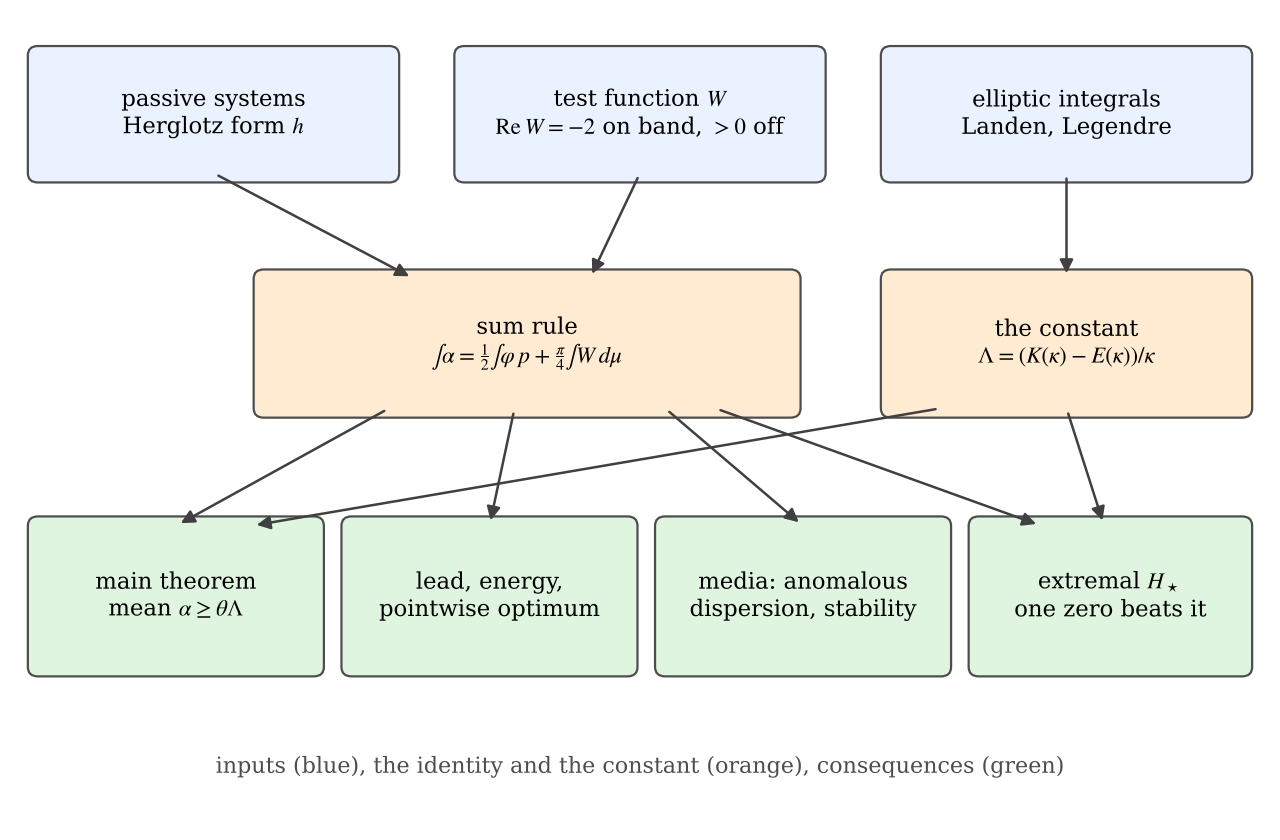
\includegraphics[width=\columnwidth]{figures/fig_roadmap.png}
\caption{How the results depend on each other. The sum rule
(\cref{thm:sumrule}) is built from the test function $W$ (\cref{sec:test});
the constant $\Lambda$ comes from the moments of the weight
(\cref{sec:constant}); every later statement is a consequence of these two
or of the extremal system of \cref{thm:extremal}.}
\label{fig:roadmap}
\end{figure}

\begin{figure}[t]
\centering
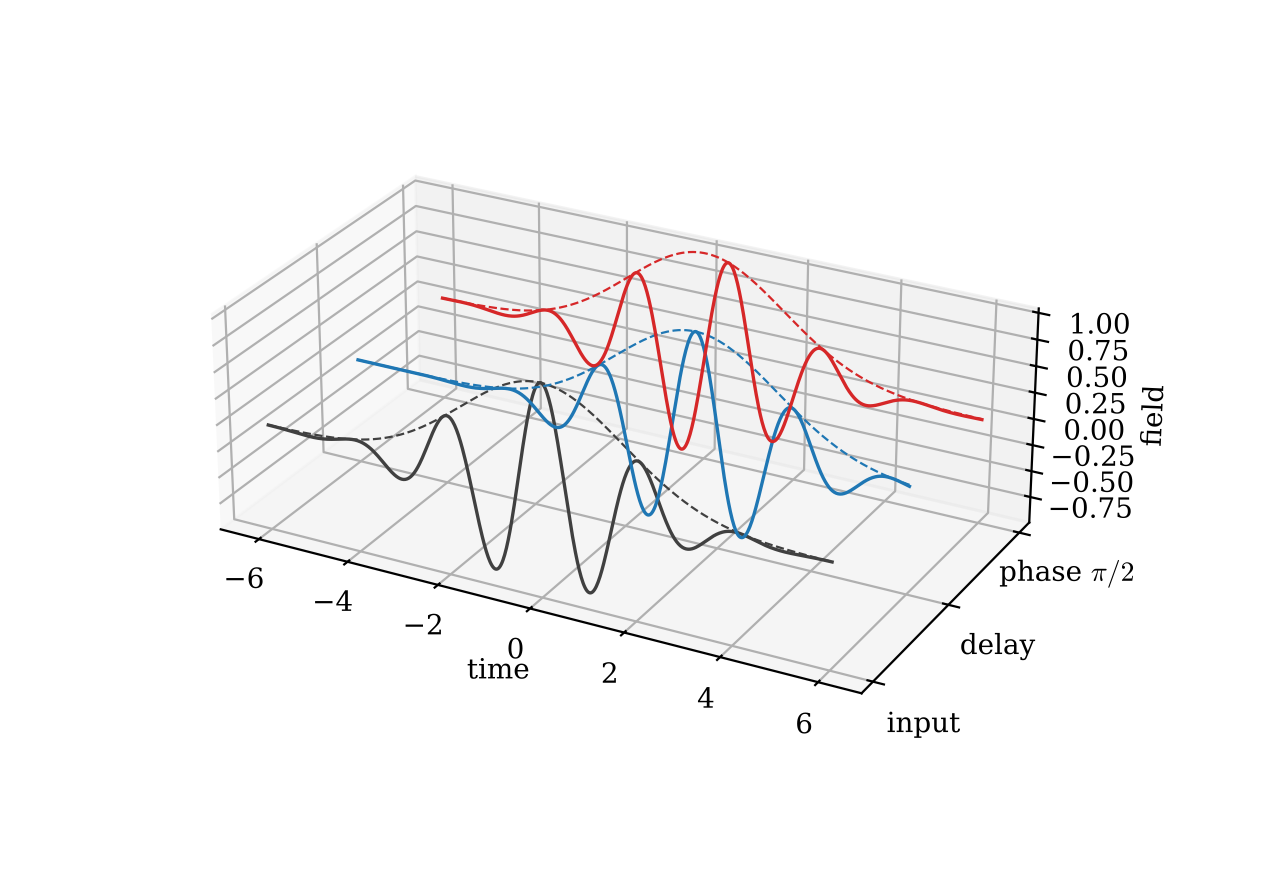
\includegraphics[width=\columnwidth]{figures/fig_pulses.png}
\caption{A pulse (grey), the same pulse after a delay (blue), and after a
constant phase shift of $\pi/2$ on its whole band (red). Dashed curves are the
envelopes. The delay moves the envelope and the oscillations together; the
constant phase shift moves the oscillations under a fixed envelope. Only the
second operation costs energy in a passive system.}
\label{fig:pulses}
\end{figure}

\section{The equations of the earlier paper}\label{sec:audit}

We first go through the formulas of \cite{tb23}, since the rest of the paper
replaces them. They fall into two groups: kinematic relations between phase,
time and frequency, which are correct, and formulas for an energy loss
$\Delta E$, which are not.

\subsection{Phase, time and frequency}

For a sinusoid of frequency $f$, a delay $\Delta t$ produces the phase
\begin{equation}\label{eq:audit-phase}
\Phi^\circ=360^\circ f\,\Delta t ,
\end{equation}
and \cite{tb23} rewrites this as $\Delta t=\Phi^\circ/(360^\circ f)$ and
$f=\Phi^\circ/(360^\circ\Delta t)$. These are correct, with the
understanding that the last one gives the frequency at which a \emph{given}
delay produces a \emph{given} phase; it does not describe a change of
frequency. The delay that produces one degree is
\[
T(\mathrm{deg})=\frac{1}{360f},
\]
which at $f=5$\,MHz is $555.6$\,ps, as stated in \cite{tb23}. Two of the
phrasings there should be read with care. The equation ``$1^\circ$ phase
shift $=T/360$'' equates an angle with a time; what is meant is that a delay
of $T/360$ produces a phase of $1^\circ$, where $T=1/f$ is the period. The
name ``time distortion'' for $\Delta t$ suggests something more than a delay;
the quantity in \eqref{eq:audit-phase} is just the delay. Finally, the
statement that $T(\mathrm{deg})\propto1/f$ is true of the delay needed for one
degree, and it is the reason why a delay cannot produce the same phase at
two frequencies.

\subsection{The energy formulas}

The paper \cite{tb23} proposes three formulas for an ``infinitesimal loss of
wave energy'',
\begin{equation}\label{eq:audit-dE}
\begin{gathered}
\Delta E=hf\Delta t,\qquad
\Delta E=\frac{2\pi hf_1}{360}\,T(\mathrm{deg}),\\
\Delta E=\frac{2\pi h}{360}\,\frac{T(\mathrm{deg})}{\Delta t},
\end{gathered}
\end{equation}
with $h$ Planck's constant, and evaluates the first one for $f=4{,}986{,}111.11$\,Hz and
$\Delta t=555$\,ps. Four things go wrong.

\emph{Units.} Planck's constant is an action, measured in J\,s; $hf$ is an
energy and $hf\Delta t$ is again an action. The same holds for the other two
formulas in \eqref{eq:audit-dE}, in which $T(\mathrm{deg})/\Delta t$ is a pure
number and $f_1T(\mathrm{deg})$ is the number $1/360$. None of the three
expressions is an energy.\footnote{If $T(\mathrm{deg})$ is read as the angle
$1^\circ=\pi/180$ rather than as a time, the second formula has units of
energy, but it then reads $\Delta E=(\pi/180)\,hf_1\,(2\pi/360)$, a fixed
multiple of $hf_1$ without any connection to the delay.}

\emph{Arithmetic.} The product evaluated in \cite{tb23} is
\[
(6.626\times10^{-34})(4.986\times10^{6})(555\times10^{-12})
=1.834\times10^{-36},
\]
in J\,s, not $1.848\times10^{-27}$\,J. The stated value is larger by a factor
of about $10^{9}$, and it would amount to $56\%$ of the energy
$E_1=hf_1=3.313\times10^{-27}$\,J of a quantum at $5$\,MHz, which can hardly
be called infinitesimal.

\emph{A fixed phase shift does not change the frequency.} The second example
of \cite{tb23} assigns to a $1^\circ$ phase shift the new frequency
$f_2=f_1-f_1/360=4{,}986{,}111.11$\,Hz. Multiplying a wave by a constant
$e^{i\theta}$, or delaying it, leaves its frequency unchanged
(\cref{prop:static}). A frequency change of $f_1/360$ occurs when the phase
\emph{slips} by one degree in every period, that is, when the phase grows
at the rate $\dot\theta=2\pi f_1/360$ (\cref{prop:slip}). In that case the
energy of a quantum changes by
\[
E_1-E_2=\frac{hf_1}{360}=9.20\times10^{-30}\ \mathrm J ,
\]
and this is the only energy difference of the size suggested by the example.
The paper also gives $E_2=hf_2\approx3.313\times10^{-27}$\,J; the correct
value is $3.304\times10^{-27}$\,J, and the difference from $E_1$ is the number
just computed, not $1.848\times10^{-27}$\,J.

\emph{What $hf$ measures.} The energy $hf$ is that of one quantum. The energy
of a classical wave is fixed by its amplitude, which the formulas
\eqref{eq:audit-dE} do not contain. A loss caused by a passive element is a
fraction of the incident energy, whether the wave is classical or quantised,
and the quantity to compute is therefore the transmission $\abs{H}^2$, or,
per quantum, the probability of absorption.

\subsection{What remains}

\Cref{tab:audit} lists the corrections. The kinematic part of \cite{tb23}
stands. The energy part asks a good question in the wrong variables: the
phase shift that has a price is the one applied uniformly over a band, the
price is a fraction of the energy rather than a multiple of $h$, and its
size is governed by the bandwidth. Sections~\ref{sec:passive}--\ref{sec:waves}
compute it.

\begin{table}[t]
\caption{The formulas of \cite{tb23} and their status.}
\label{tab:audit}
\centering
\small
\begin{tabular}{@{}p{0.43\columnwidth}p{0.51\columnwidth}@{}}
\toprule
Formula in \cite{tb23} & Status \tabularnewline
\midrule
\raggedright $\Phi^\circ=360^\circ f\Delta t$ and its inversions & \raggedright correct\tabularnewline
\raggedright $T(\mathrm{deg})=1/(360f)$, $555$\,ps at $5$\,MHz & \raggedright correct\tabularnewline
\raggedright ``$1^\circ$ phase shift $=T/360$'' & \raggedright angle equated with time; a delay $T/360$ gives $1^\circ$\tabularnewline
\raggedright $\Delta E=hf\Delta t$ & \raggedright an action, in J\,s; its value is $1.83\times10^{-36}$, not $1.848\times10^{-27}$\tabularnewline
\raggedright $\Delta E=(2\pi hf_1/360)T(\mathrm{deg})$ & \raggedright an action; equals $2\pi h/360^2$\tabularnewline
\raggedright $\Delta E=(2\pi h/360)\,T(\mathrm{deg})/\Delta t$ & \raggedright an action\tabularnewline
\raggedright $f_2=f_1-f_1/360$ after a $1^\circ$ shift & \raggedright only if the phase slips $1^\circ$ per period\tabularnewline
\raggedright $E_2\approx3.313\times10^{-27}$\,J & \raggedright $3.304\times10^{-27}$\,J; $E_1-E_2=9.20\times10^{-30}$\,J\tabularnewline
\bottomrule
\end{tabular}
\end{table}

\section{Phase, delay and frequency}\label{sec:kinematics}

\subsection{Conventions}

A signal is a real function $s(t)$ of finite energy, with Fourier transform
$\hat s(\omega)=\int_\R s(t)e^{i\omega t}\dd t$, so that
$\hat s(-\omega)=\overline{\hat s(\omega)}$. A linear time-invariant system
acts by $\widehat{s_{\rm out}}=H\hat s_{\rm in}$. With this convention a
delay by $\tau$ has $H(\omega)=e^{i\omega\tau}$, so a positive phase of $H$
is a \emph{lag}, and causality means that $H$ extends analytically to the
upper half-plane $\Cp=\{\Im z>0\}$ (\cref{sec:passive}). The analytic signal
of $s$ is
\[
\psi(t)=\frac1\pi\int_0^\infty\hat s(\omega)e^{-i\omega t}\dd\omega ,
\qquad s=\Re\psi .
\]
For a narrowband pulse we write $\psi(t)=A(t)e^{-i(\omega_0t+\phi)}$ with a
slowly varying envelope $A\ge0$, a carrier frequency $\omega_0$ and a
carrier--envelope phase $\phi$. The phase $\phi$ locates the crests of the
carrier relative to the peak of the envelope; it is the quantity controlled
in frequency combs \cite{telle,apolonski}.\footnote{In a mode-locked laser $\phi$ advances by a fixed amount from one pulse to the next; the rate of this slip is the carrier--envelope offset frequency of the comb, which is measured and locked in \cite{telle,apolonski}.}

Three different operations go under the name of a phase shift. We treat
them in turn.

\subsection{A constant phase factor}

The \emph{ideal phase shifter} by $\theta$ multiplies every positive
frequency by $e^{i\theta}$ and, to keep the signal real, every negative
frequency by $e^{-i\theta}$:
\begin{equation}\label{eq:ideal}
H_\theta(\omega)=e^{i\theta\operatorname{sgn}\omega},\qquad
\psi_{\rm out}=e^{i\theta}\psi .
\end{equation}
It is not causal.\footnote{With our Fourier convention the multiplier $i\operatorname{sgn}\omega$ has the kernel $1/(\pi t)$, since $\PV\int\operatorname{sgn}\omega\,e^{-i\omega t}\dd\omega=-2i/t$. Hence $H_\theta=\cos\theta+i\sin\theta\operatorname{sgn}\omega$ has the impulse response $\cos\theta\,\delta(t)+\sin\theta/(\pi t)$, which does not vanish for $t<0$ unless $\sin\theta=0$.}

\begin{proposition}\label{prop:static}
The ideal phase shifter preserves the energy $\int s^2\dd t$, the power
spectrum $\abs{\hat s}^2$ and hence every frequency present in the signal.
For a single quantised mode of frequency $\omega$ the operator
$U=e^{-i\theta N}$, $N$ the number operator, commutes with the Hamiltonian
$\hbar\omega(N+\frac12)$, so the probability distribution of the energy is
unchanged. If $\sin\theta\ne0$, the ideal phase shifter is not causal.
\end{proposition}

\begin{proof}
The first statements follow from $\abs{H_\theta}=1$ and Parseval's
identity, and from $[N,U]=0$. For the last, $H_\theta=\cos\theta
+i\sin\theta\operatorname{sgn}\omega$, and $i\operatorname{sgn}\omega$ is the
transfer function of convolution with the Hilbert kernel $\pm1/(\pi t)$,
which does not vanish for $t<0$.
\end{proof}

So a phase shift, as such, neither changes the frequency nor costs energy.
What it costs is causality, and the price of restoring causality in a
passive system is the subject of the rest of the paper.

\subsection{A delay}

A delay $\tau$ gives $\psi_{\rm out}(t)=\psi(t-\tau)$ and the phase
$\omega\tau$ at frequency $\omega$, which is the relation
\eqref{eq:audit-phase}. It is causal and lossless, and it realises any
prescribed phase at one frequency. On a band it realises a phase that is
proportional to frequency, never a constant one.

\subsection{A phase that changes in time}

Let a device multiply the analytic signal by $e^{i\theta(t)}$.

\begin{proposition}\label{prop:slip}
If $\theta(t)=\theta_0+\Omega t$, then
$\widehat{\psi_{\rm out}}(\omega)=e^{i\theta_0}\hat\psi(\omega+\Omega)$: the
spectrum is moved down by $\Omega$, and a component of frequency $\omega$ leaves
with frequency $\omega-\Omega$ and energy $\hbar(\omega-\Omega)$ per
quantum. If the device conserves the number of quanta, the energy of the
signal changes by the fraction $\Omega/\omega$ at each frequency, the
difference being exchanged with the agent that drives $\theta$.
\end{proposition}

\begin{proof}
The Fourier transform of $e^{i\Omega t}\psi(t)$ is $\hat\psi(\omega+\Omega)$
in our convention. The rest is the relation $E=\hbar\omega$ for each
quantum.
\end{proof}

The conservation of the number of quanta is what the Manley--Rowe relations
\cite{manley} give for a lossless parametric modulator, and the linear phase
ramp is the serrodyne frequency translator \cite{cumming}. A phase that slips
by one degree per period has $\Omega=\omega/360$; at $5$\,MHz this is a shift
of $13{,}888.89$\,Hz and an energy of $hf/360=9.20\times10^{-30}$\,J per
quantum, the numbers of \cref{sec:audit}. This is the only reading under
which a ``$1^\circ$ phase shift'' changes frequency. It is an active
operation, not a passive one.

\subsection{Constant phase on a band}

The operation that keeps the envelope and moves the carrier is the following.

\begin{proposition}\label{prop:cep}
Let $0<a<b$ and let $H$ satisfy $H(-\omega)=\overline{H(\omega)}$ and
\begin{equation}\label{eq:affine}
H(\omega)=e^{-\alpha(\omega)}e^{i(\theta+\tau\omega)},\qquad a\le\omega\le b .
\end{equation}
If the spectrum of $s$ lies in $[-b,-a]\cup[a,b]$ and $\alpha=0$ on $[a,b]$,
then $\psi_{\rm out}(t)=e^{i\theta}\psi(t-\tau)$. In particular a pulse
$A(t)e^{-i(\omega_0t+\phi)}$ leaves as $A(t-\tau)e^{-i(\omega_0(t-\tau)+\phi-\theta)}$:
the envelope is delayed by $\tau$ and the carrier--envelope phase is moved
by $-\theta$. Conversely, if $\psi_{\rm out}=e^{i\theta}\psi(\cdot-\tau)$ for
every such signal, then \eqref{eq:affine} holds with $\alpha=0$.
\end{proposition}

\begin{proof}
On positive frequencies $\widehat{\psi_{\rm out}}=H\hat\psi
=e^{i\theta}e^{i\tau\omega}\hat\psi$, which is the transform of
$e^{i\theta}\psi(t-\tau)$. The converse follows by testing with signals whose
spectra are concentrated near each $\omega\in[a,b]$.
\end{proof}

The phase of $H$ on the band is then $\varphi(\omega)=\theta+\tau\omega$. Its
slope $\tau$ is the group delay; its intercept
\[
\theta=\varphi(\omega)-\omega\varphi'(\omega)=\omega\big(\tau_{\rm ph}-\tau_{\rm gr}\big),
\qquad \tau_{\rm ph}=\frac{\varphi}{\omega},\ \tau_{\rm gr}=\varphi',
\]
is the carrier--envelope offset, $\omega$ times the excess of phase delay
over group delay. A delay has $\theta=0$. The main theorem says that a passive
zero-free system can have $\theta>0$ only by attenuating, on average over the
band, at least $\theta\Lambda$ nepers.

\section{Passive systems and Herglotz functions}\label{sec:passive}

\subsection{Passive systems}

\begin{definition}\label{def:passive}
A \emph{passive system} is a function $H$ analytic in $\Cp$ with
$\abs{H(z)}\le1$ there and with the real symmetry
$H(-\bar z)=\overline{H(z)}$. Its frequency response is the boundary
function $H(\omega)=\lim_{\varepsilon\downarrow0}H(\omega+i\varepsilon)$,
which exists for almost every real $\omega$.\footnote{Fatou's theorem: a bounded analytic function in $\Cp$ has nontangential limits at almost every point of $\R$ \cite[Ch.~I]{garnett}.}
\end{definition}

The definition encodes three physical requirements. A time-invariant
system that never puts out more energy than it receives acts on signals of
finite energy by a multiplier of norm at most one; causality makes the
multiplier the boundary value of a bounded analytic function in $\Cp$; and a
real impulse response gives the symmetry. That these requirements are
equivalent to \cref{def:passive} is classical \cite{toll,nussenzveig,garnett}.
The transmission coefficient of a passive two-port, the reflection
coefficient of a passive one-port and the propagation factor of a passive
medium (\cref{sec:waves}) are passive systems.

The zeros of a passive system that is not identically zero satisfy the
Blaschke condition, and $H=BG$ where $B$ is the Blaschke product of the
zeros and $G$ is passive and has no zeros in $\Cp$ \cite[Ch.~II]{garnett}.
Since the zeros of $H$ come in pairs $\zeta,-\bar\zeta$, $B$ can be chosen
with the real symmetry.\footnote{With $B_\zeta(z)=(z-\zeta)/(z-\bar\zeta)$ one has $B_\zeta(-\bar z)=\overline{B_{-\bar\zeta}(z)}$, so the product $B_\zeta B_{-\bar\zeta}$ has the symmetry, and so does the Blaschke product over such pairs, with the usual unimodular convergence factors chosen in pairs.} We call $H$ \emph{zero-free} when $B$ is constant.
This includes every minimum-phase system, and also the singular inner
functions, which are not minimum-phase in the usual sense: the factor
$\exp(i\gamma/(\omega_0-z))$, $\gamma>0$, is the lossless resonance of a
reactance at $\omega_0$ in the sense of Foster \cite{foster}.

\subsection{The Herglotz function of a zero-free system}

A \emph{Herglotz function} is an analytic map $h$ from $\Cp$ to the closed
upper half-plane. Every such function has the representation
\cite{nussenzveig,garnett,bernland}
\begin{equation}\label{eq:herglotz}
h(z)=c+\beta z+\int_\R\Big(\frac1{t-z}-\frac t{1+t^2}\Big)\dd\mu(t),
\end{equation}
with $c\in\R$, $\beta\ge0$ and a positive measure $\mu$ with
$\int\dd\mu/(1+t^2)<\infty$. The measure is recovered by the Stieltjes
inversion formula,
\begin{equation}\label{eq:stieltjes}
\mu\big((x_1,x_2)\big)+\tfrac12\mu(\{x_1,x_2\})
=\lim_{y\downarrow0}\frac1\pi\int_{x_1}^{x_2}\Im h(x+iy)\dd x,
\end{equation}
and $\beta=\lim_{y\to\infty}h(iy)/(iy)$.

\begin{lemma}\label{lem:log}
Let $H$ be a zero-free passive system, $H\not\equiv0$. There are a sign
$\sigma\in\{1,-1\}$ and a unique Herglotz function $h$ with
\begin{equation}\label{eq:Hh}
H=\sigma e^{ih},\qquad h(iy)\in i\R\ (y>0),\qquad h(-\bar z)=-\overline{h(z)} .
\end{equation}
In the representation \eqref{eq:herglotz} of $h$ one has $c=0$ and $\mu$ is
even, so that
\begin{equation}\label{eq:foster}
h(z)=\beta z-\frac{\mu(\{0\})}{z}+\int_{(0,\infty)}\frac{2z}{t^2-z^2}\dd\mu(t).
\end{equation}
\end{lemma}

\begin{proof}
On the imaginary axis $H(iy)=\overline{H(iy)}$ is real and, having no zeros,
of constant sign $\sigma$. Since $\Cp$ is simply connected, $\sigma H$ has an
analytic logarithm, which we fix to be real on $i\R_+$. Put
$h=-i\log(\sigma H)$. Then $\Im h=-\log\abs H\ge0$, so $h$ is a Herglotz
function, and $h(iy)\in i\R$. The function $g(z)=-\overline{h(-\bar z)}$ is
analytic, satisfies $e^{ig}=\overline{\sigma H(-\bar z)}=\sigma H=e^{ih}$, and
agrees with $h$ on $i\R_+$; hence $g=h$. In \eqref{eq:herglotz}, $c=\Re h(i)=0$;
the symmetry and \eqref{eq:stieltjes} show that $\mu$ is even, and pairing
$t$ with $-t$ in \eqref{eq:herglotz} gives \eqref{eq:foster}. Uniqueness holds
because two such logarithms differ by a constant in $2\pi\Z$ that vanishes
on $i\R_+$.
\end{proof}

We call
\begin{gather*}
\varphi(\omega)=\Re h(\omega+i0),\\
\alpha(\omega)=\Im h(\omega+i0)=-\log\abs{H(\omega)}
\end{gather*}
the \emph{phase} and the \emph{attenuation} of $H$. Then $\arg H(\omega)
=\varphi(\omega)+\frac{1-\sigma}2\pi$ modulo $2\pi$. The phase $\varphi$ is the
argument of $\sigma H$ continued from the imaginary axis, where it vanishes;
when $H$ is continuous and positive at $\omega=0$ and nonzero on $[0,b]$, it
is simply the argument of $H$ unwrapped from $\varphi(0)=0$. The
representation \eqref{eq:foster} separates the three ingredients of a
zero-free system: the delay $\beta z$, the lossless resonances, which are the
atoms and the singular part of $\mu$, and the losses, which are the
absolutely continuous part of $\mu$, with density $\alpha/\pi$.

\subsection{The band}

Fix $0<a<b$ and write $S=[-b,-a]\cup[a,b]$.

\begin{definition}\label{def:band}
A zero-free passive system $H$ is \emph{regular on the band} if there is an
open interval $I\supset[a,b]$, $I\subset(0,\infty)$, such that $H$ extends
continuously to $\Cp\cup I$ and has no zeros on $I$.
\end{definition}

\begin{lemma}\label{lem:regular}
If $H$ is regular on the band, then $h$ extends continuously to $\Cp\cup I$,
$\varphi$ and $\alpha$ are continuous on $I$, and the restriction of $\mu$ to
$I\cup(-I)$ is $\pi^{-1}\alpha(\abs t)\dd t$. In particular $\mu$ has no
atoms at $\pm a,\pm b$.
\end{lemma}

\begin{proof}
Near each point of $I$ the function $\sigma H$ is continuous and nonzero, so
its logarithm, normalised as in \cref{lem:log}, is continuous up to $I$. The
convergence in \eqref{eq:stieltjes} is then uniform on compact subintervals
of $I$, which gives $\mu=\pi^{-1}\alpha\dd t$ on $I$; evenness gives the
statement on $-I$.
\end{proof}

\subsection{Lossless bands}

The following is the form of Foster's reactance theorem \cite{foster} that we
need.

\begin{proposition}\label{prop:foster}
Let $H=B\sigma e^{ih}$ be passive, with $B$ a real-symmetric Blaschke
product whose zeros stay away from $I$, and let $\sigma e^{ih}$ be regular on
the band. If $\abs{H}=1$ on $I$, then the argument of $H$ is real-analytic
and nondecreasing on $I$, and strictly increasing unless $H$ is constant.
\end{proposition}

\begin{proof}
On $I$ we have $\alpha=0$, so by \cref{lem:regular} $\mu$ vanishes on $I$
and \eqref{eq:foster} continues analytically across $I$, with
\[
\varphi'(x)=\beta+\frac{\mu(\{0\})}{x^2}+\int_{(0,\infty)\setminus I}
\frac{2(t^2+x^2)}{(t^2-x^2)^2}\dd\mu(t)\;\ge\;0 .
\]
Each factor $(z-\zeta)/(z-\bar\zeta)$ of $B$, $\Im\zeta>0$, has argument with
derivative $2\Im\zeta/\abs{x-\zeta}^2>0$ on the real line, and the series for
$B$ converges with its derivatives on $I$. The sum is strictly positive
unless $\beta=0$, $\mu=0$ and $B$ is constant.
\end{proof}

\begin{corollary}\label{cor:rigid}
Under the hypotheses of \cref{prop:foster}, a passive system that is
lossless on $I$ and has constant argument on $[a,b]$ is a constant,
$H\equiv\pm1$.
\end{corollary}

So constant phase on a band is impossible without loss. The main theorem
measures how much loss.

\section{A test function for the band}\label{sec:test}

\subsection{The functions $\rho$ and $W$}

Let
\[
\rho(z)=\Big(\frac{z-a}{z-b}\Big)^{1/2}\Big(\frac{z+a}{z+b}\Big)^{1/2},
\qquad z\in\Cp,
\]
with principal square roots. The map $z\mapsto(z-a)/(z-b)$ is a real
M\"obius transformation of determinant $a-b<0$ and sends $\Cp$ onto the lower
half-plane; $z\mapsto(z+a)/(z+b)$ has determinant $b-a>0$ and sends $\Cp$ onto
itself. Neither meets the negative real axis, so $\rho$ is analytic and
zero-free in $\Cp$.\footnote{The principal square root is analytic and zero-free on $\C\setminus(-\infty,0]$, and an open half-plane bounded by the real axis does not meet $(-\infty,0]$.} Put
\begin{equation}\label{eq:W}
W(z)=\rho(z)-2+\frac1{\rho(z)}=\frac{(\rho(z)-1)^2}{\rho(z)} ,
\end{equation}
and, for $a<t<b$,
\begin{equation}\label{eq:p}
\begin{gathered}
r(t)=\sqrt{(t^2-a^2)(b^2-t^2)},\\
p(t)=\frac{a^2+b^2-2t^2}{r(t)}
=\sqrt{\frac{b^2-t^2}{t^2-a^2}}-\sqrt{\frac{t^2-a^2}{b^2-t^2}} .
\end{gathered}
\end{equation}

\begin{lemma}\label{lem:W}
\begin{enumerate}
\item[(i)] $\rho(-\bar z)=\overline{\rho(z)}$, and
$\rho(z)=1+\frac{b^2-a^2}{2z^2}+O(z^{-4})$, so $W(z)=O(z^{-4})$ as
$z\to\infty$ in $\overline{\Cp}$.
\item[(ii)] $\rho$ and $W$ extend continuously to $\overline{\Cp}$ minus the
four points $\pm a,\pm b$, near which $\abs{W(z)}=O(\abs{z\mp a}^{-1/2})$,
$O(\abs{z\mp b}^{-1/2})$.
\item[(iii)] On $\R\setminus S$, $\rho$ is real and positive, and
$W=(\rho-1)^2/\rho$ is real and strictly positive.
\item[(iv)] For $a<t<b$, $\rho(t+i0)=-i\,s(t)$ with
$s(t)=\sqrt{(t^2-a^2)/(b^2-t^2)}$, hence
\[
W(t)=-2+i\,p(t),\qquad W(-t)=-2-i\,p(t).
\]
\end{enumerate}
\end{lemma}

\begin{proof}
(i) The symmetry holds for each factor. Since
$\rho^2=(z^2-a^2)/(z^2-b^2)=1+(b^2-a^2)/(z^2-b^2)$ and $\rho\to1$, the
expansion follows, and $W=(\rho-1)^2/\rho$.
(ii) Near $b$ the factor $(z-a)/(z-b)$ behaves like a constant over $z-b$,
so $\rho\sim c(z-b)^{-1/2}$ and $W\sim\rho$; near $a$, $\rho\sim c(z-a)^{1/2}$ and
$W\sim1/\rho$. The points $-a,-b$ follow by symmetry.
(iii) For real $t\notin S$ both quotients are positive.
(iv) For $a<t<b$ and $\varepsilon\downarrow0$ the number
$(t-a)/(t-b+i\varepsilon)$ has negative real part and negative imaginary
part, so its principal square root tends to $-i\sqrt{(t-a)/(b-t)}$, while
$\sqrt{(t+a)/(t+b)}$ is positive. Hence $\rho=-is$ and
$W=-is-2+i/s=-2+i(1/s-s)=-2+ip$. The value at $-t$ follows from (i).
\end{proof}

\Cref{fig:testfunction} shows $\Re W$: a plateau at $-2$ over the band,
positive values elsewhere, and integrable spikes at the band edges.

\begin{figure}[t]
\centering
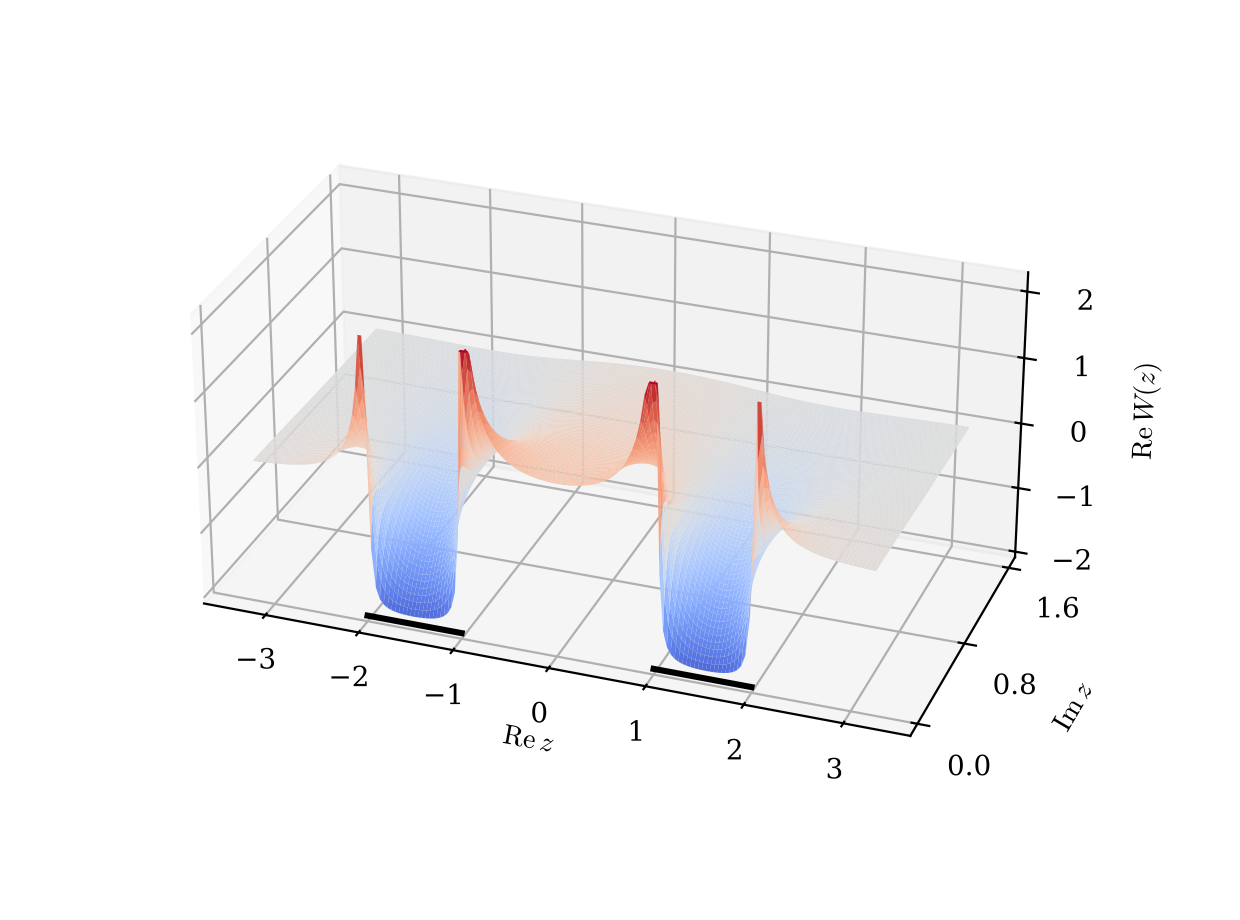
\includegraphics[width=\columnwidth]{figures/fig_testfunction.png}
\caption{The real part of the test function $W$ over the upper half-plane
for $a=1$, $b=2$ (values clipped at $\pm2.2$). On the real axis it equals $-2$
on the band (black segments) and is strictly positive elsewhere.}
\label{fig:testfunction}
\end{figure}

\subsection{The kernel identity}

\begin{lemma}\label{lem:kernel}
For $s>0$, $s\ne a,b$,
\begin{equation}\label{eq:kernel}
\frac1\pi\PV\int_a^b p(x)\,\frac{2x}{x^2-s^2}\dd x=
\begin{cases}-2,& a<s<b,\\ W(s),& s\notin[a,b].\end{cases}
\end{equation}
\end{lemma}

\begin{proof}
Apply Cauchy's theorem to $W(z)/(z-s)$ on the boundary of the half-disc of
radius $R$ in $\Cp$, indented by semicircles of radius $\varepsilon$ above
$s,\pm a,\pm b$. By \cref{lem:W}(ii) the small semicircles at $\pm a,\pm b$
contribute $O(\varepsilon^{1/2})$; by \cref{lem:W}(i) the large one
contributes $O(R^{-4})$; the one at $s$ contributes $-\pi iW(s)$ in the
limit, $W$ being continuous at $s$. Therefore
\[
\PV\int_\R\frac{W(x)}{x-s}\dd x=\pi i\,W(s).
\]
Taking imaginary parts and using that $\Im W$ vanishes off $S$ and equals
$\pm p(\abs x)$ on $\pm[a,b]$ (\cref{lem:W}(iii),(iv)),
\begin{align*}
\pi\Re W(s)&=\PV\int_a^bp(x)\Big(\frac1{x-s}+\frac1{x+s}\Big)\dd x\\
&=\PV\int_a^bp(x)\frac{2x}{x^2-s^2}\dd x .
\end{align*}
By \cref{lem:W}, $\Re W(s)=-2$ for $a<s<b$ and $\Re W(s)=W(s)$ otherwise.
\end{proof}

\begin{figure}[t]
\centering
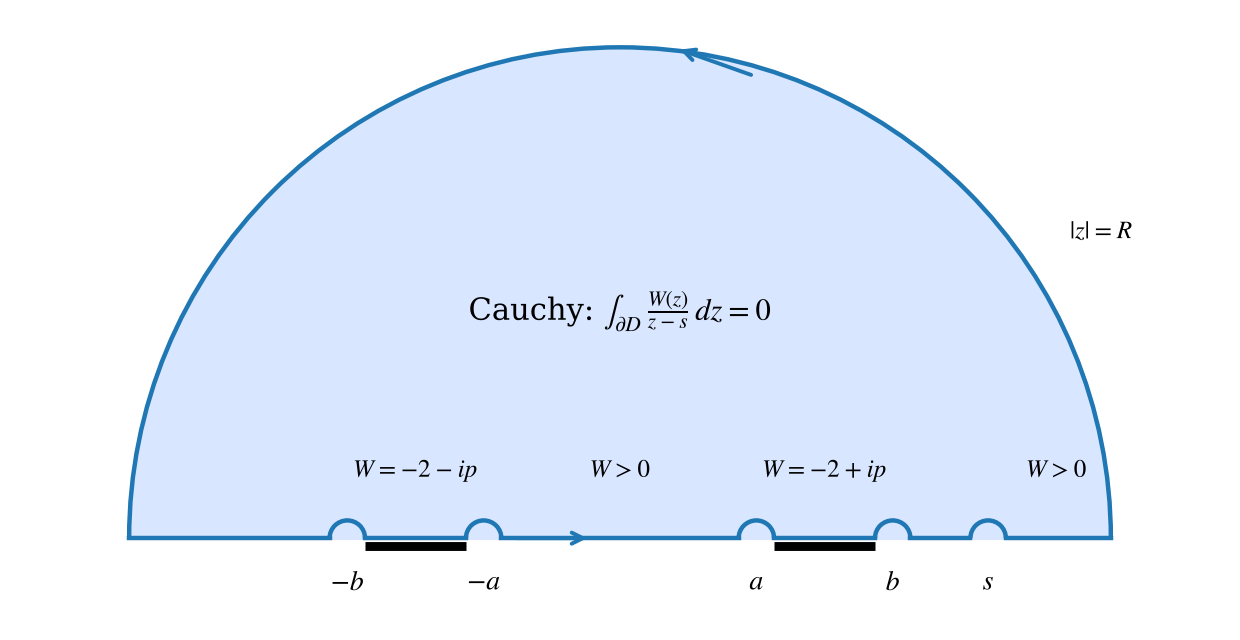
\includegraphics[width=\columnwidth]{figures/fig_contour.png}
\caption{The contour of the proof of \cref{lem:kernel}: a half-disc of
radius $R$ in $\Cp$, indented above the branch points $\pm a,\pm b$ of $W$
and above the pole $s$. The branch cuts of $W$ are the two bands $\pm[a,b]$
(thick); the indentations at the branch points contribute nothing in the
limit, the one at $s$ contributes $-\pi iW(s)$.}
\label{fig:contour}
\end{figure}

\subsection{Moments of the weight}

The weight $p$ is positive on $(a,c)$ and negative on $(c,b)$, where
$c^2=(a^2+b^2)/2$. Under $\sigma=x^2$ it becomes antisymmetric, and this
gives all the sign information we need.

\begin{lemma}\label{lem:moments}
Let $A=a^2$, $B=b^2$ and
$\varpi(\sigma)=(A+B-2\sigma)/\sqrt{(\sigma-A)(B-\sigma)}$, so that
$x\,p(x)\dd x=\frac12\varpi(x^2)\dd(x^2)$.
\begin{enumerate}
\item[(i)] $\varpi(A+B-\sigma)=-\varpi(\sigma)$, and $\int_a^bx\,p(x)\dd x=0$.
\item[(ii)] If $f$ is continuous and nonincreasing on $[A,B]$, then
$\int_a^bx\,p(x)f(x^2)\dd x\ge0$, with equality only for constant $f$.
\item[(iii)] $J:=\int_a^bp(x)\dd x>0$ and $\int_a^b\frac{p(x)}{x}\dd x
=\frac{\pi(b-a)^2}{2ab}$.
\item[(iv)] $\int_a^bx^{2j+1}p(x)\dd x<0$ for $j\ge1$, and
$\int_a^bx^3p(x)\dd x=-\frac\pi8(b^2-a^2)^2$.
\end{enumerate}
\end{lemma}

\begin{proof}
(i) The antisymmetry is visible, and it gives $\int_A^B\varpi=0$.
(ii) With $\sigma_m=(A+B)/2$,
\[
\int_a^bxpf(x^2)\dd x=\frac12\int_A^{\sigma_m}\varpi(\sigma)
\big(f(\sigma)-f(A+B-\sigma)\big)\dd\sigma ,
\]
and both factors are nonnegative for $\sigma<\sigma_m$; the integral vanishes
only if $f(\sigma)=f(A+B-\sigma)$ throughout, which for a monotone $f$ means
$f$ constant.
(iii) Apply (ii) to $f(\sigma)=\sigma^{-1/2}$ and $f(\sigma)=\sigma^{-1}$. The
value follows from the elementary integrals
\begin{gather*}
\int_A^B\frac{\dd\sigma}{\sqrt{(\sigma-A)(B-\sigma)}}=\pi,\\
\int_A^B\frac{\dd\sigma}{\sigma\sqrt{(\sigma-A)(B-\sigma)}}=\frac{\pi}{\sqrt{AB}},
\end{gather*}
which give $\frac12\big((A+B)\pi/\sqrt{AB}-2\pi\big)=\pi(b-a)^2/(2ab)$.
(iv) Apply (ii) to $f(\sigma)=-\sigma^j$. For $j=1$ use also
$\int_A^B\sigma\,\dd\sigma/\sqrt{\cdot}=\pi(A+B)/2$ and
$\int_A^B\sigma^2\dd\sigma/\sqrt\cdot=\pi(3A^2+2AB+3B^2)/8$.
\end{proof}

The first moment vanishing is the reason why delays are free; the positivity
of $J$ is the reason why a constant phase lag is not.

\section{The sum rule and the main theorem}\label{sec:sumrule}

\subsection{The sum rule}

\begin{theorem}\label{thm:sumrule}
Let $H=\sigma e^{ih}$ be a zero-free passive system that is regular on the
band, with phase $\varphi$, attenuation $\alpha$ and Herglotz measure $\mu$.
Then
\begin{equation}\label{eq:sumrule}
\int_a^b\alpha(\omega)\dd\omega
=\frac12\int_a^b\varphi(\omega)\,p(\omega)\dd\omega
+\frac\pi4\int_{\R\setminus S}W(t)\dd\mu(t),
\end{equation}
and every term is finite. The last integral is nonnegative, and it vanishes
if and only if $\mu(\R\setminus S)=0$.
\end{theorem}

The proof uses one fact about the Hilbert transform $\mathcal Hf(x)=\pi^{-1}
\PV\int f(t)\dd t/(x-t)$ on the line, the antisymmetry
\begin{equation}\label{eq:riesz}
\int_\R f\,\mathcal Hg\dd x=-\int_\R(\mathcal Hf)\,g\dd x ,
\qquad f\in L^{q},\ g\in L^{q'},
\end{equation}
valid for $1<q<\infty$ by M.~Riesz's theorem \cite{titchmarsh,king}.\footnote{Riesz's theorem is the boundedness of $\mathcal H$ on $L^q$, $1<q<\infty$. For smooth compactly supported $f,g$ the antisymmetry is Fubini's theorem for the truncated kernel $\mathbf 1_{\abs{x-t}>\varepsilon}/(x-t)$, which is odd under $x\leftrightarrow t$; it extends to $L^q\times L^{q'}$ by density and Riesz's bound.}

\begin{proof}
\emph{Finiteness.} $\varphi$ is continuous on $[a,b]$ and $p$ is integrable.
On $I\setminus[a,b]$ the measure is $\pi^{-1}\alpha\dd t$ with $\alpha$
bounded (\cref{lem:regular}), and $W$ has integrable singularities at
$a,b$. Away from $I\cup(-I)$, $W$ is bounded and $O(t^{-4})$, while
$\int\dd\mu/(1+t^2)<\infty$.

\emph{Decomposition.} Choose $a_1<a$ and $b_1>b$ with $[a_1,b_1]\subset I$,
let $I_1=(a_1,b_1)$, and split $\mu=\mu_1+\mu_2$ with $\mu_1$ the restriction
of $\mu$ to $I_1\cup(-I_1)$. By \eqref{eq:foster},
\begin{gather*}
h=\beta z+h_1+h_2,\\
h_j(z)=-\frac{\mu_j(\{0\})}{z}+\int_{(0,\infty)}\frac{2z}{t^2-z^2}\dd\mu_j(t),
\end{gather*}
and $\varphi=\beta x+\Re h_1+\Re h_2$ on $(a,b)$.

\emph{The delay.} $\frac12\int_a^b\beta x\,p(x)\dd x=0$ by
\cref{lem:moments}(i).

\emph{The far part.} The measure $\mu_2$ has no mass in $I_1\cup(-I_1)$, so
$h_2$ is continuous up to $(a,b)$ and the kernel $2x/(t^2-x^2)$ is bounded by
a constant times $(1+t^2)^{-1}$ for $x\in[a,b]$ and $t\notin I_1$. Fubini's
theorem and \cref{lem:kernel,lem:moments}(iii) give
\begin{align*}
\frac12\int_a^b\Re h_2\,p\dd x
&=-\frac{\mu(\{0\})}2\int_a^b\frac px\dd x-\frac\pi2\int_{(0,\infty)\setminus I_1}W\dd\mu\\
&=-\frac\pi4\int_{\R\setminus(I_1\cup-I_1)}W\dd\mu ,
\end{align*}
where we used $W(0)=(b-a)^2/(ab)$,\footnote{$\rho(0)=\sqrt{a/b}\sqrt{a/b}=a/b$, so $W(0)=a/b-2+b/a=(b-a)^2/(ab)$. With \cref{lem:moments}(iii), $\int_a^bp/x\dd x=\pi(b-a)^2/(2ab)=\frac\pi2W(0)$, which turns the atom at $0$ into $-\frac\pi4W(0)\mu(\{0\})$.} the evenness of $W$ on $\R\setminus S$
and of $\mu$.

\emph{The near part.} Here $\mu_1=\psi(t)\dd t$ with $\psi=\pi^{-1}\alpha(\abs
t)$ on $I_1\cup(-I_1)$, a bounded function. For almost every $x\in(a,b)$,
\begin{align*}
\Re h_1(x)&=\PV\int_{I_1}\psi(t)\frac{2x}{t^2-x^2}\dd t\\
&=\PV\int_{I_1}\psi(t)\Big(\frac1{t-x}-\frac1{t+x}\Big)\dd t ,
\end{align*}
the boundary value of the real part of a Cauchy integral with bounded
density \cite{king,muskhelishvili}. We claim that
\begin{multline}\label{eq:swap}
\int_a^bp(x)\,\Re h_1(x)\dd x\\
=\int_{I_1}\psi(t)\Big(\PV\int_a^bp(x)\frac{2x}{t^2-x^2}\dd x\Big)\dd t .
\end{multline}
For the part $1/(t+x)$ of the kernel this is Fubini's theorem, the kernel
being bounded. For the part $1/(t-x)$ it is \eqref{eq:riesz} with
$f=p\,\mathbf 1_{[a,b]}\in L^{3/2}$ and $g=\psi\mathbf 1_{I_1}\in L^{3}$; the
function $p$ lies in $L^q$ for every $q<2$ because its singularities are of
order $\abs{x-a}^{-1/2}$ and $\abs{x-b}^{-1/2}$. By \cref{lem:kernel}
the inner integral in \eqref{eq:swap} equals $2\pi$ for $t\in(a,b)$ and
$-\pi W(t)$ for $t\in I_1\setminus[a,b]$. Hence
\begin{align*}
\frac12\int_a^bp\,\Re h_1\dd x&=\pi\int_a^b\psi\dd t-\frac\pi2\int_{I_1\setminus[a,b]}W\dd\mu\\
&=\int_a^b\alpha\dd t-\frac\pi4\int_{(I_1\cup-I_1)\setminus S}W\dd\mu .
\end{align*}

Adding the three parts gives \eqref{eq:sumrule}. Since $W>0$ on $\R\setminus
S$ and $\mu$ has no atoms at $\pm a,\pm b$, the last term vanishes exactly
when $\mu(\R\setminus S)=0$.
\end{proof}

The identity \eqref{eq:sumrule} holds for every phase. Its content is that
the band loss is a fixed linear functional of the band phase plus a
nonnegative price for everything the system does outside the band: a
lossless resonance at $\omega_0\notin[a,b]$ with weight $\gamma$ in $\mu$ costs
$\frac\pi2W(\omega_0)\gamma$,\footnote{The measure is even, so the resonance puts mass $\gamma$ at both $\pm\omega_0$, and $W(-\omega_0)=W(\omega_0)$ off the band; the two atoms give $\frac\pi4\cdot2W(\omega_0)\gamma$.} a pole at the origin costs
$\frac\pi4W(0)\mu(\{0\})$, and absorption outside the band costs its
$W$-weighted total.

\subsection{Constant phase lag}

Put
\begin{equation}\label{eq:Lambda}
\begin{aligned}
\Lambda&=\frac{J}{2(b-a)}\\
&=\frac1{2(b-a)}\int_a^b
\frac{a^2+b^2-2\omega^2}{\sqrt{(\omega^2-a^2)(b^2-\omega^2)}}\dd\omega>0 .
\end{aligned}
\end{equation}
\Cref{sec:constant} shows $\Lambda=(K(\kappa)-E(\kappa))/\kappa$.

\begin{theorem}[Main theorem]\label{thm:main}
Let $H$ be a zero-free passive system, regular on the band $[a,b]$, whose
phase on the band is
\[
\varphi(\omega)=\theta+\tau\omega,\qquad a<\omega<b,
\]
with $\theta\ge0$ and $\tau\in\R$. Then
\begin{equation}\label{eq:main}
\frac1{b-a}\int_a^b\alpha(\omega)\dd\omega\ \ge\ \theta\,\Lambda .
\end{equation}
Equality holds if and only if $\mu(\R\setminus S)=0$; for every $\theta\ge0$
it is attained by the system $H_\star$ of \cref{thm:extremal}.
\end{theorem}

\begin{proof}
By \cref{lem:moments}(i),
$\frac12\int_a^b(\theta+\tau\omega)p\dd\omega=\frac12\theta J=(b-a)\theta\Lambda$,
and \cref{thm:sumrule} gives the inequality and the case of equality.
\end{proof}

Three remarks make the statement concrete.

\begin{remark}[Constant argument]\label{rem:arg}
If $\arg H\equiv\theta$ modulo $2\pi$ on the band, then
$\varphi=\theta-\frac{1-\sigma}2\pi$ modulo $2\pi$, and since $\varphi$ is
continuous it is a constant $\theta'$ with $\theta'\equiv\theta\pmod\pi$. The
theorem applies with $\theta'$ when $\theta'>0$. Which representative occurs
is not decided by the band: it depends on how much phase the system has
accumulated from the imaginary axis, for instance from zero frequency.
\end{remark}

\begin{remark}[Lossless resonances]\label{rem:resonances}
The equality case shows that every lossless resonance outside the band, and
every atom of $\mu$ at zero frequency, raises the loss strictly above the
bound. Shaping the phase with reactances, the classical tool of all-pass and
phase-equaliser design, therefore works against a constant phase lag.
\Cref{fig:cost} shows the price of a unit of measure off the band, the
factor $\frac\pi4W(t)$ of \eqref{eq:sumrule}.
\end{remark}

\begin{figure}[t]
\centering
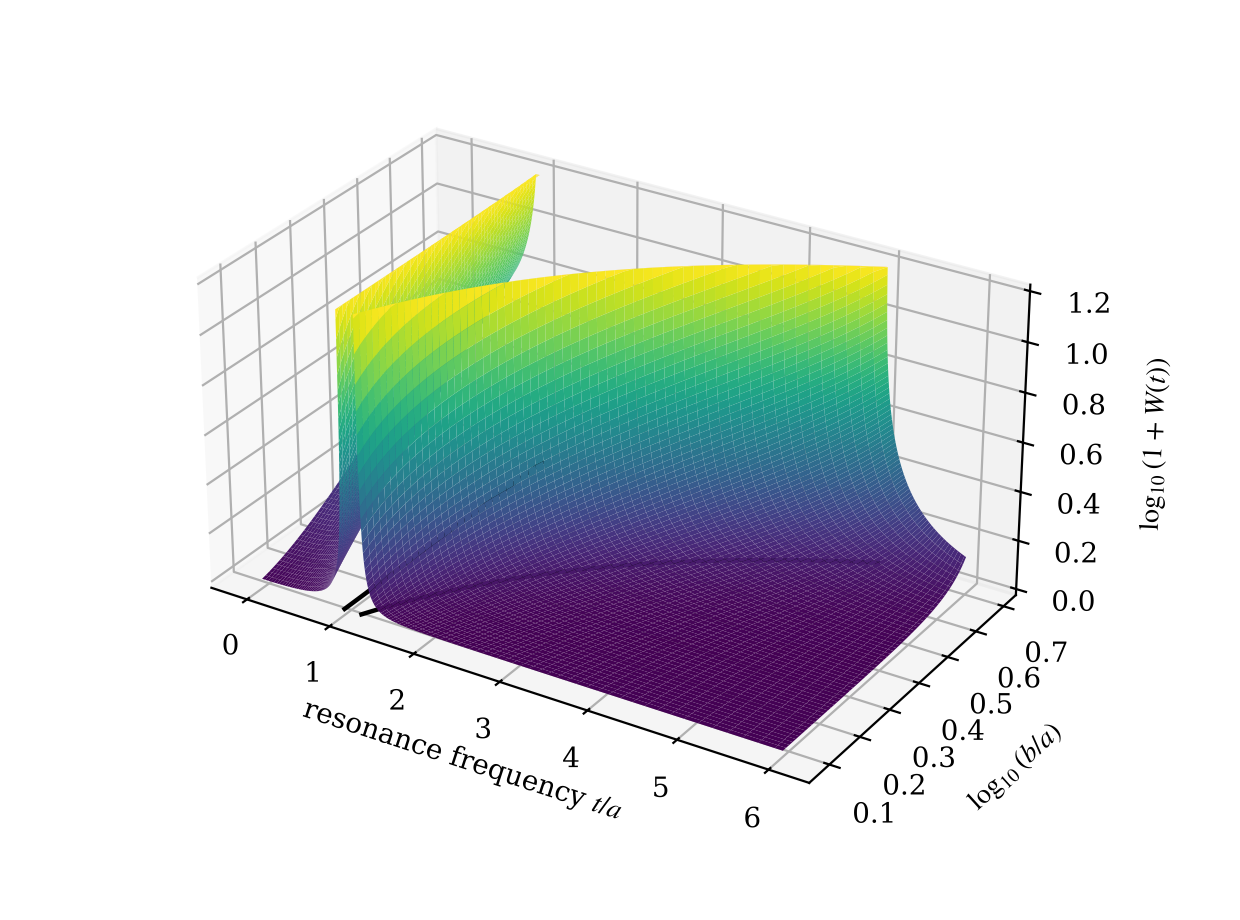
\includegraphics[width=\columnwidth]{figures/fig_cost.png}
\caption{The cost $\log_{10}(1+W(t))$ of a lossless resonance at frequency
$t$, as a function of $t/a$ and of the band ratio $b/a$. It vanishes only on
the band (the gap between the two sheets), grows without bound at the band
edges, and decays like $t^{-4}$ at high frequency (\cref{lem:W}(i)); at
$t=0$ it is $W(0)=a/b+b/a-2>0$.}
\label{fig:cost}
\end{figure}

\begin{remark}[Passivity everywhere is needed]\label{rem:cpe}
The constant-phase element $H(z)=(-iz/a)^{-\gamma}$, $0<\gamma<1$, familiar
from dielectric relaxation \cite{westerlund}, has phase $\theta=\gamma\pi/2$ at
every positive frequency and attenuation $\alpha=\gamma\log(\omega/a)\ge0$
on $[a,\infty)$. Over an octave its mean attenuation is
$(2\theta/\pi)(2\log2-1)=0.2459\,\theta$, below the bound
$0.2735\,\theta$. There is no contradiction: $\abs H>1$ for $\omega<a$, so $H$
is not passive. The bound depends on passivity at all frequencies, not only
on the band.
\end{remark}

\subsection{Constant phase lead}

For a negative intercept the same identity, applied after an inversion of
the frequency axis, gives a weighted bound.

\begin{theorem}\label{thm:lead}
Let $H$ be as in \cref{thm:main} but with $\theta<0$. Then
\begin{equation}\label{eq:lead}
\frac1{b-a}\int_a^b\alpha(\omega)\,\frac{ab}{\omega^2}\dd\omega
\ \ge\ \abs\theta\,\Lambda-\frac\pi4\,\tau\,(b-a).
\end{equation}
For $\tau=0$ equality holds if and only if $\beta=0$ and $\mu$ vanishes on
$\R\setminus(S\cup\{0\})$; it is attained by $H_\star(-ab/z)$, where $H_\star$
is the extremal system for $\abs\theta$.
\end{theorem}

\begin{proof}
The map $z\mapsto-ab/z$ preserves $\Cp$, so $\tilde h(z)=h(-ab/z)$ is a
Herglotz function with the symmetry of \eqref{eq:Hh}, and $\tilde H=\sigma
e^{i\tilde h}$ is zero-free, passive and regular on the band, since
$x\mapsto ab/x$ maps a neighbourhood of $[a,b]$ onto another. For $x\in(a,b)$
the point $-ab/(x+i0)$ lies above $-ab/x\in(-b,-a)$, so by the oddness of
$\varphi$,
\[
\tilde\varphi(x)=-\varphi(ab/x),\qquad\tilde\alpha(x)=\alpha(ab/x).
\]
Substituting $x=ab/\omega$ and using $r(ab/\omega)=ab\,r(\omega)/\omega^2$,
\begin{gather*}
\int_a^bf(ab/x)\,p(x)\dd x=\int_a^bf(\omega)\,p^*(\omega)\dd\omega,\\
p^*(\omega)=\frac{a^2+b^2-2a^2b^2/\omega^2}{r(\omega)},
\end{gather*}
for every integrable $f$. With $f=1$ and $f(\omega)=\omega$ this gives
$\int_a^bp^*=J$ and $\int_a^b\omega p^*=ab\int_a^bp/x=\pi(b-a)^2/2$
(\cref{lem:moments}(iii)). \Cref{thm:sumrule} for $\tilde H$ now reads
\[
\int_a^b\alpha(\omega)\frac{ab}{\omega^2}\dd\omega
=-\frac12\int_a^b(\theta+\tau\omega)p^*\dd\omega+\frac\pi4\int_{\R\setminus S}W\dd\tilde\mu ,
\]
which is \eqref{eq:lead} after division by $b-a$. The measure $\tilde\mu$
is the image of $\mu$ under $t\mapsto-ab/t$ with density $ab/t^2$ on
$\R\setminus\{0\}$, plus an atom $ab\beta$ at $0$ coming from the term
$\beta z$; an atom of $\mu$ at $0$ becomes a linear term of $\tilde h$ and
costs nothing. This gives the case of equality, and $H_\star(-ab/z)$ has
$\beta=0$ and its measure on $S\cup\{0\}$.
\end{proof}

\subsection{The worst frequency}

\begin{corollary}\label{cor:worst}
Let $H$ be zero-free, passive and regular on the band, with $\arg
H\equiv\theta$ modulo $2\pi$ on $[a,b]$. Then
\[
\max_{[a,b]}\alpha\ \ge\ \dist(\theta,\pi\Z)\,\Lambda ,
\]
so at some frequency of the band the transmitted power is at most
$e^{-2\dist(\theta,\pi\Z)\Lambda}$. If the phase $\theta'$ of
\cref{rem:arg} is positive, also
\[
\exp\Big(\frac1{b-a}\int_a^b\log\abs{H(\omega)}^2\dd\omega\Big)\le e^{-2\theta'\Lambda},
\]
that is, the geometric mean of the power transmission over the band is at
most $e^{-2\theta'\Lambda}$.
\end{corollary}

\begin{proof}
By \cref{rem:arg} the phase is a constant $\theta'\equiv\theta\pmod\pi$. If
$\theta'>0$ then $\theta'\ge\dist(\theta,\pi\Z)$ and \cref{thm:main} bounds
the mean, hence the maximum, of $\alpha$. If $\theta'<0$ then
$\abs{\theta'}\ge\dist(\theta,\pi\Z)$, and since
$\int_a^bab\,\omega^{-2}\dd\omega=b-a$ the left side of \eqref{eq:lead}
with $\tau=0$ is at most $\max\alpha$. The
second statement is \eqref{eq:main} with $\log\abs H=-\alpha$.
\end{proof}

\begin{remark}[The lead extremal]\label{rem:leadmean}
For the system $H_\star(-ab/z)$ of \cref{thm:lead}, whose phase is
$-\abs\theta$ on the band, \cref{thm:sumrule} applied directly gives the
plain mean attenuation
\[
\frac1{b-a}\int_a^b\alpha\dd\omega
=\abs\theta\,\frac{E(\kappa)-\kappa'^2K(\kappa)}{\kappa},\qquad\kappa'^2=1-\kappa^2,
\]
because its measure off $S$ is the atom $ab\,\tau_\star$ at $0$, of cost
$\frac\pi4W(0)ab\tau_\star$, with $\tau_\star$ from \cref{thm:extremal} and the
evaluation of \cref{sec:constant}. For an octave this is $0.2656\abs\theta$,
slightly below $\Lambda=0.2735$. Whether it is the least plain mean among
systems with constant phase lead is not known.
\end{remark}

\section{The constant}\label{sec:constant}

We use the complete elliptic integrals of modulus $k\in[0,1)$,
\begin{gather*}
K(k)=\int_0^{\pi/2}\frac{\dd\phi}{\sqrt{1-k^2\sin^2\phi}},\\
E(k)=\int_0^{\pi/2}\sqrt{1-k^2\sin^2\phi}\,\dd\phi ,
\end{gather*}
and the moduli attached to the band,
\[
k=\sqrt{1-a^2/b^2},\qquad k'=a/b,\qquad
\kappa=\frac{b-a}{b+a}=\frac{1-k'}{1+k'} .
\]
The facts on $K$ and $E$ that we use are collected in \cref{app:elliptic}.

\begin{proposition}\label{prop:J}
With $I_0=\int_a^b\dd t/r(t)$ and $I_2=\int_a^bt^2\dd t/r(t)$,
\[
I_0=\frac{K(k)}b,\qquad I_2=b\,E(k),
\]
and
\begin{equation}\label{eq:J}
\begin{aligned}
J&=(a^2+b^2)I_0-2I_2=b\big[(1+k'^2)K(k)-2E(k)\big]\\
&=2(a+b)\big[K(\kappa)-E(\kappa)\big].
\end{aligned}
\end{equation}
Consequently
\begin{equation}\label{eq:Lambda-closed}
\Lambda=\frac{K(\kappa)-E(\kappa)}{\kappa}.
\end{equation}
\end{proposition}

\begin{proof}
Substitute $t^2=b^2-(b^2-a^2)\sin^2\phi$, $0\le\phi\le\pi/2$. Then
$b^2-t^2=(b^2-a^2)\sin^2\phi$, $t^2-a^2=(b^2-a^2)\cos^2\phi$,
$t\dd t=-(b^2-a^2)\sin\phi\cos\phi\dd\phi$, hence $\dd t/r(t)=-\dd\phi/t$ and
$t=b\sqrt{1-k^2\sin^2\phi}$. This gives $I_0$ and $I_2$, and the second form of
$J$. The Landen transformation (\cref{app:elliptic}) states
\[
K(k)=(1+\kappa)K(\kappa),\qquad E(k)=(1+k')E(\kappa)-k'K(k).
\]
Inserting these,\footnote{The coefficient of $K(\kappa)$ is $b(1+\kappa)\big[(1+k'^2)+2k'\big]=b(1+\kappa)(1+k')^2$, the term $2k'$ coming from $-2E(k)$.} and using $b(1+\kappa)=2b^2/(a+b)$ and $1+k'=(a+b)/b$,
\begin{align*}
J&=b(1+\kappa)(1+k')^2K(\kappa)-2b(1+k')E(\kappa)\\
&=2(a+b)\big[K(\kappa)-E(\kappa)\big].
\end{align*}
Dividing by $2(b-a)=2\kappa(a+b)$ gives \eqref{eq:Lambda-closed}.
\end{proof}

\begin{proposition}\label{prop:Lambda}
\begin{enumerate}
\item[(i)] With $c_n=\binom{2n}{n}4^{-n}$,
\[
\Lambda=\frac\pi2\sum_{n\ge1}\frac{2n}{2n-1}\,c_n^2\,\kappa^{2n-1}
=\frac\pi4\kappa\Big(1+\frac38\kappa^2+\frac{15}{64}\kappa^4+\cdots\Big),
\]
a series with positive coefficients;\footnote{By \eqref{eq:KEseries}, $K-E=\frac\pi2\sum_{n\ge1}c_n^2\big(1-\frac1{1-2n}\big)\kappa^{2n}$ and $1-\frac1{1-2n}=\frac{2n}{2n-1}$; dividing by $\kappa$ gives (i).} in particular $\Lambda$ increases with
$\kappa$, that is, with $b/a$.
\item[(ii)] For all $0<a<b$,
\[
\frac\pi4\,\frac{b-a}{b+a}\ <\ \Lambda\ \le\ \frac\pi4\,\frac{\kappa}{1-\kappa^2}
=\frac\pi{16}\,\frac{b^2-a^2}{ab}.
\]
\item[(iii)] As $a/b\to0$,
$\Lambda=\log\frac{4}{\kappa'}-1+o(1)=\frac12\log\frac{4b}{a}-1+o(1)$,
with $\kappa'=\sqrt{1-\kappa^2}=2\sqrt{ab}/(a+b)$.
\end{enumerate}
\end{proposition}

\begin{proof}
(i) From $K=\frac\pi2\sum c_n^2\kappa^{2n}$ and
$E=\frac\pi2\sum c_n^2\kappa^{2n}/(1-2n)$ one gets
$K-E=\frac\pi2\sum_{n\ge1}c_n^2\kappa^{2n}\,2n/(2n-1)$. The coefficients for
$n=1,2,3$ are $\frac12$, $\frac3{16}$ and $\frac{15}{128}$, which give the
displayed expansion after division by $\kappa$.
(ii) The lower bound is the first term. For the upper bound, the ratio of
consecutive coefficients $d_n=c_n^2\,2n/(2n-1)$ is
\[
\frac{d_{n+1}}{d_n}=\frac{(2n+1)(2n-1)}{(2n+2)\,2n}<1,
\]
so $d_n\le d_1=\frac12$ and $K-E\le\frac\pi4\sum_{n\ge1}\kappa^{2n}
=\frac\pi4\kappa^2/(1-\kappa^2)$. Finally $\kappa/(1-\kappa^2)=(b^2-a^2)/(4ab)$.
(iii) As $\kappa\to1$, $K(\kappa)=\log(4/\kappa')+o(1)$ and $E(\kappa)\to1$
(\cref{app:elliptic}); and $\log(4/\kappa')=\log\big(2(a+b)/\sqrt{ab}\big)
=\frac12\log(4b/a)+o(1)$.
\end{proof}

For a narrow band with centre $\bar\omega=(a+b)/2$ and width
$\Delta\omega=b-a$, $\kappa=\Delta\omega/(2\bar\omega)$, so
\begin{equation}\label{eq:narrow}
\Lambda=\frac\pi8\,\frac{\Delta\omega}{\bar\omega}
\Big(1+O\big((\Delta\omega/\bar\omega)^2\big)\Big).
\end{equation}
The bound is linear in the relative bandwidth, which is what one expects: on
an infinitely narrow band a delay achieves any phase without loss. For wide
bands it grows only logarithmically in $b/a$. \Cref{tab:lambda} gives values,
also in decibels per degree of phase, which is $\Lambda$ times
$(20/\ln 10)(\pi/180)=0.15160$, and \cref{fig:bound} shows the bound as a
surface.

\begin{table}[t]
\caption{The constant $\Lambda$ of \eqref{eq:Lambda-closed}, the least mean
attenuation per radian of constant phase lag, for several band ratios. The
last column is the least worst-frequency power loss for $\theta=1^\circ$.}
\label{tab:lambda}
\centering
\small
\begin{tabular}{@{}rrrrr@{}}
\toprule
$b/a$ & $\kappa$ & $\Lambda$ (Np/rad) & dB/deg & $1-e^{-2\Lambda\pi/180}$ \\
\midrule
$1.01$ & $0.004975$ & $0.003907$ & $0.000592$ & $1.36\times10^{-4}$\\
$1.1$  & $0.04762$  & $0.03743$  & $0.00567$  & $1.31\times10^{-3}$\\
$1.5$  & $0.2$      & $0.1595$   & $0.0242$   & $5.55\times10^{-3}$\\
$2$    & $0.3333$   & $0.2735$   & $0.0415$   & $9.50\times10^{-3}$\\
$3$    & $0.5$      & $0.4366$   & $0.0662$   & $1.51\times10^{-2}$\\
$10$   & $0.8182$   & $0.9448$   & $0.143$    & $3.24\times10^{-2}$\\
$100$  & $0.9802$   & $2.016$    & $0.306$    & $6.80\times10^{-2}$\\
$1000$ & $0.9980$   & $3.150$    & $0.478$    & $1.04\times10^{-1}$\\
\bottomrule
\end{tabular}
\end{table}

\begin{figure}[t]
\centering
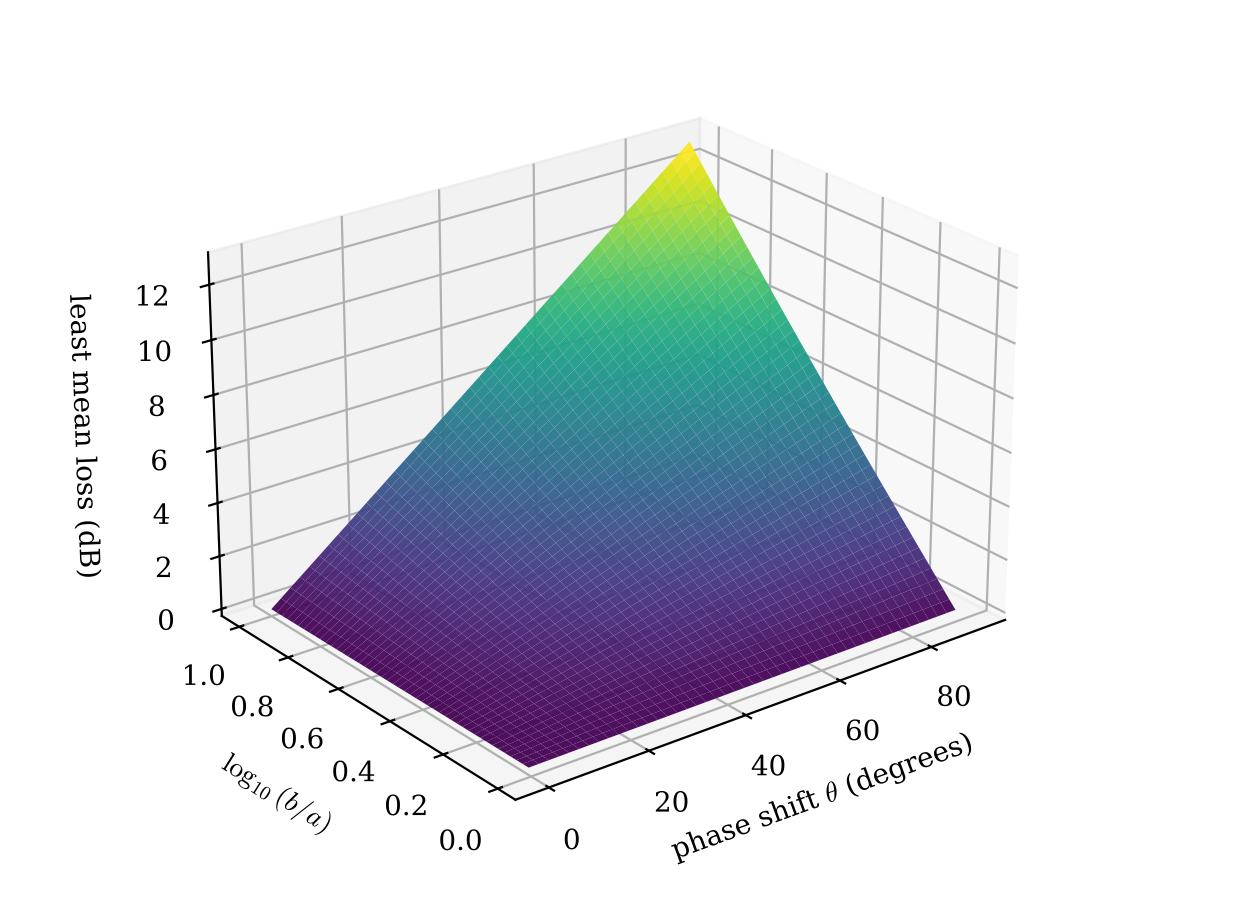
\includegraphics[width=\columnwidth]{figures/fig_bound.png}
\caption{The least mean loss $\theta\Lambda$, in decibels, over the phase lag
$\theta$ and the band ratio $b/a$. The surface is linear in $\theta$ and
increasing in $b/a$.}
\label{fig:bound}
\end{figure}

\section{Sharpness: the extremal systems}\label{sec:extremal}

\subsection{The square root $R$}

Let $R$ be the branch of $\sqrt{(z^2-a^2)(z^2-b^2)}$ that is analytic in
$\C\setminus S$ and satisfies $R(z)=z^2\big(1+O(z^{-2})\big)$ at infinity. It
exists because a loop around one component of $S$ encircles two branch
points.\footnote{Each of the four factors $(z\mp a)^{1/2}$, $(z\mp b)^{1/2}$ changes sign along a loop around its branch point; a loop around $[a,b]$ changes the sign twice, so the product returns to its value.}

\begin{lemma}\label{lem:R}
$R(-z)=R(z)$ and $R(\bar z)=\overline{R(z)}$. On the real axis,
$R(t)=\sqrt{(t^2-a^2)(t^2-b^2)}>0$ for $\abs t>b$,
$R(t)=-\sqrt{(a^2-t^2)(b^2-t^2)}<0$ for $\abs t<a$, and
\[
R(t+i0)=i\,r(t),\quad R(-t+i0)=-i\,r(t)\qquad(a<t<b).
\]
\end{lemma}

\begin{proof}
The symmetries hold because $R(-z)$ and $\overline{R(\bar z)}$ are branches of
the same root with the same behaviour at infinity. Near $z=b$,
$R(z)=(z-b)^{1/2}G(z)$ with $G$ analytic and $G(b)=\sqrt{2b(b^2-a^2)}>0$, the
root being positive for $z>b$. Passing from $t>b$ to $t<b$ through $\Cp$ turns
$(z-b)^{1/2}$ into $i\sqrt{b-t}$, so $R=ir$ on $(a,b)$. Near $z=a$ write
$R=(z-a)^{1/2}G_1(z)$ with $(z-a)^{1/2}>0$ for $t>a$; then $G_1$ is
positive imaginary on $(a,b)$, and passing to $t<a$ through $\Cp$ gives
$R=i\sqrt{a-t}\,G_1<0$. The values on the negative axis follow from the
symmetries.
\end{proof}

\subsection{The extremal system for constant phase}

Put
\begin{equation}\label{eq:m-tau}
m^2=b^2\,\frac{E(k)}{K(k)},\qquad
\tau_\star=\frac{2\theta K(k)}{\pi b}=\frac{4\theta K(\kappa)}{\pi(a+b)} ,
\end{equation}
so that $a^2<m^2<b^2$, because $m^2=I_2/I_0$ is an average of $t^2$ over
$(a,b)$ (\cref{prop:J}), and define
\begin{equation}\label{eq:hstar}
h_\star(z)=\tau_\star\int_0^z\frac{s^2-m^2}{R(s)}\dd s,\qquad H_\star=e^{ih_\star}.
\end{equation}

\begin{theorem}\label{thm:extremal}
Let $\theta>0$.
\begin{enumerate}
\item[(i)] The integral \eqref{eq:hstar} does not depend on the path in
$\C\setminus S$; $h_\star$ is analytic there, odd, real on $\R\setminus S$,
and $h_\star(z)=\tau_\star z+O(z^{-1})$ at infinity.
\item[(ii)] On the band, $h_\star(x+i0)=\theta+i\alpha_\star(x)$ with
\begin{equation}\label{eq:alphastar}
\alpha_\star(x)=\tau_\star\int_a^x\frac{m^2-s^2}{r(s)}\dd s ,
\end{equation}
which is positive on $(a,b)$, vanishes at $a$ and $b$, and is largest at
$x=m$.
\item[(iii)] $h_\star$ is a Herglotz function, and $H_\star$ is a zero-free
passive system, regular on the band, lossless on $\R\setminus S$, with
constant phase $\theta$ on $[a,b]$ and
\[
\frac1{b-a}\int_a^b\alpha_\star(\omega)\dd\omega=\theta\Lambda .
\]
\end{enumerate}
\end{theorem}

\begin{proof}
(i) The integrand is even, analytic in $\C\setminus S$, and integrable at the
four branch points. A loop around $[a,b]$ can be shrunk onto the two sides of
the cut, where $R=\pm ir$; its integral is $\pm2i\int_a^b(s^2-m^2)\dd s/r(s)
=\pm2i(I_2-m^2I_0)=0$. By evenness the same holds around $[-b,-a]$. Hence
$h_\star$ is single-valued, and odd. On $(-a,a)$ and on $\abs t>b$ the
integrand is real, so $h_\star$ is real there; it is also real along the
path from $0$ to $\pm a$, and the vanishing of the periods shows that it
returns to real values beyond $\pm b$. At infinity,
$(s^2-m^2)/R(s)=1+O(s^{-2})$, so $h_\star(z)-\tau_\star z$ tends to a constant;
it is odd and analytic for $\abs z>b$, so its Laurent series has only odd
powers and the constant is $0$.
(ii) For $0<x<a$, $h_\star(x)=\tau_\star\int_0^x(m^2-s^2)\dd s/\sqrt{(a^2-s^2)(b^2-s^2)}$
by \cref{lem:R}, and at $x=a$ this is
\begin{align*}
&\tau_\star\Big(\frac{m^2}bK(k')-b\big(K(k')-E(k')\big)\Big)\\
&\quad=\frac{\tau_\star b}{K(k)}\big(E(k)K(k')+E(k')K(k)-K(k)K(k')\big)\\
&\quad=\frac{\pi b\,\tau_\star}{2K(k)}=\theta ,
\end{align*}
by the substitution $s=a\sin\phi$\footnote{It gives $\dd s/\sqrt{(a^2-s^2)(b^2-s^2)}=\dd\phi/(b\sqrt{1-k'^2\sin^2\phi})$, and $\int_0^{\pi/2}\sin^2\phi\,\dd\phi/\sqrt{1-k'^2\sin^2\phi}=(K(k')-E(k'))/k'^2$ with $a^2/k'^2=b^2$.} and Legendre's relation
(\cref{app:elliptic}). Continuing from $a$ along the upper side of the cut,
where $R=ir$,
\[
h_\star(x+i0)=\theta+\tau_\star\int_a^x\frac{s^2-m^2}{ir(s)}\dd s=\theta+i\alpha_\star(x).
\]
The integrand of \eqref{eq:alphastar} is positive for $s<m$ and negative for
$s>m$, and its integral over $(a,b)$ is $I_2-m^2I_0=0$; so $\alpha_\star$
rises from $0$ at $a$ to its maximum at $m$ and falls back to $0$ at $b$.
(iii) The function $v=\Im(h_\star-\tau_\star z)$ is harmonic in $\Cp$,
continuous on $\overline{\Cp}$, tends to $0$ at infinity by (i), vanishes on
$\R\setminus S$, and equals $\alpha_\star\ge0$ on $(a,b)$ and, by the symmetry
$h_\star(-\bar z)=-\overline{h_\star(z)}$, also on $(-b,-a)$. By the minimum
principle $v\ge0$, so $\Im h_\star\ge\tau_\star\Im z\ge0$. Thus $h_\star$ is a
Herglotz function with $h_\star(iy)\in i\R$, $H_\star$ is passive and zero-free,
and it is regular on the band since $h_\star$ is continuous up to $(0,\infty)$.
As $\Im h_\star=0$ on $\R\setminus S$, \eqref{eq:stieltjes} shows
$\mu_\star(\R\setminus S)=0$, and \cref{thm:main} holds with equality.
\end{proof}

\begin{remark}\label{rem:extremal}
The extremal system is a delay $\tau_\star$ at high frequency, as its
asymptotics shows, yet its group delay on the band is zero, its phase being
constant there. All of its attenuation is in the band, and none of its
response outside the band is reactive: in the language of
\eqref{eq:foster} it has $\beta=\tau_\star$ and a measure carried by $S$. For an
octave and $\theta=1$, $\tau_\star=0.6864/a$, $m=1.4988\,a$, and the peak
attenuation is $\alpha_\star(m)=0.3482$\,Np, against the mean $0.2735$.
\Cref{fig:extremal} shows $\alpha_\star$ for several band ratios, and
\cref{fig:hstar} the function $\Im h_\star$ over $\Cp$.
\end{remark}

\begin{figure}[t]
\centering
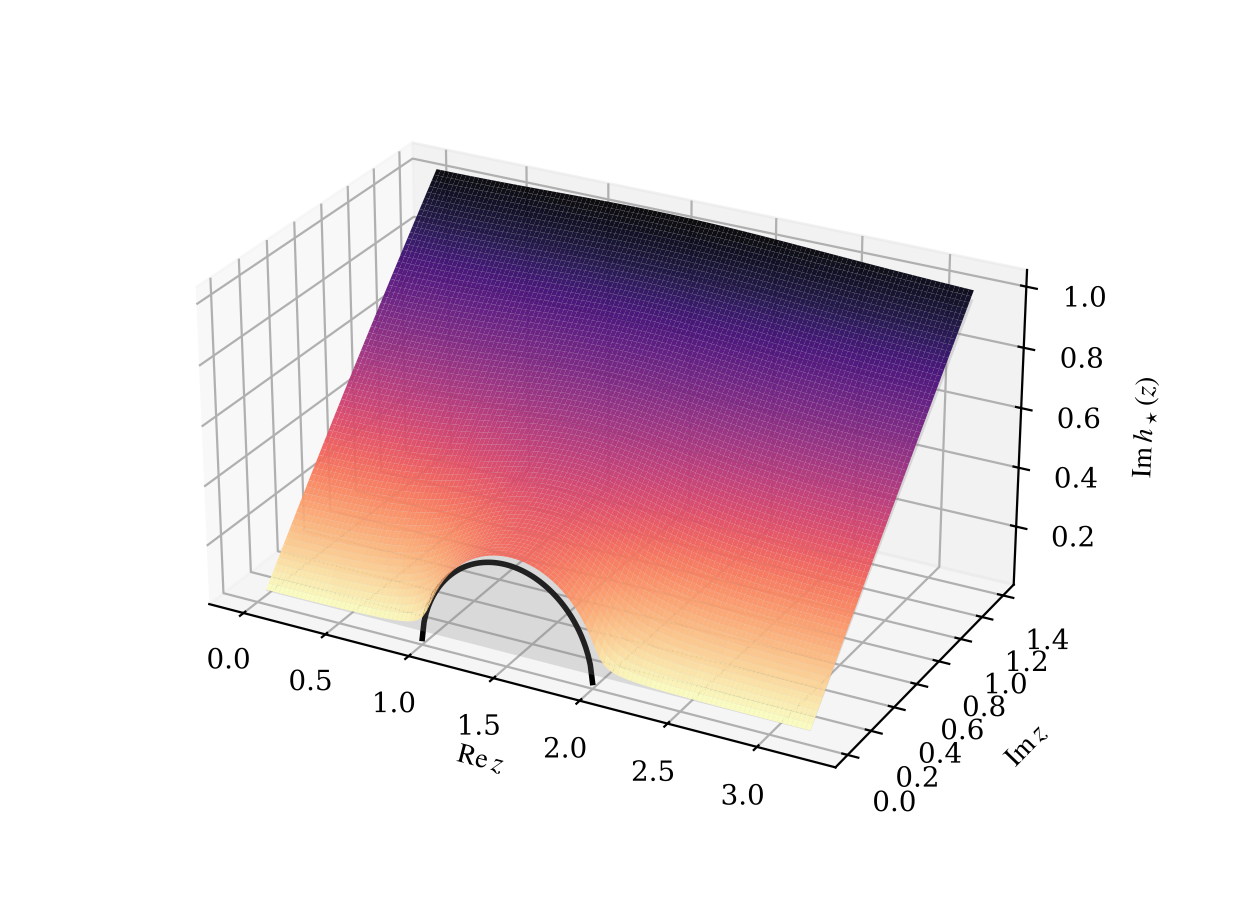
\includegraphics[width=\columnwidth]{figures/fig_hstar.png}
\caption{The surface $\Im h_\star(x+iy)$ over the upper half-plane for an
octave and $\theta=1$. It is positive in $\Cp$, as a Herglotz function must
be; on the real axis it vanishes off the band, and over the band its
boundary values are the attenuation $\alpha_\star$ (black curve). Far from
the band it approaches the plane $\tau_\star y$ (grey) of the delay.}
\label{fig:hstar}
\end{figure}

\begin{figure}[t]
\centering
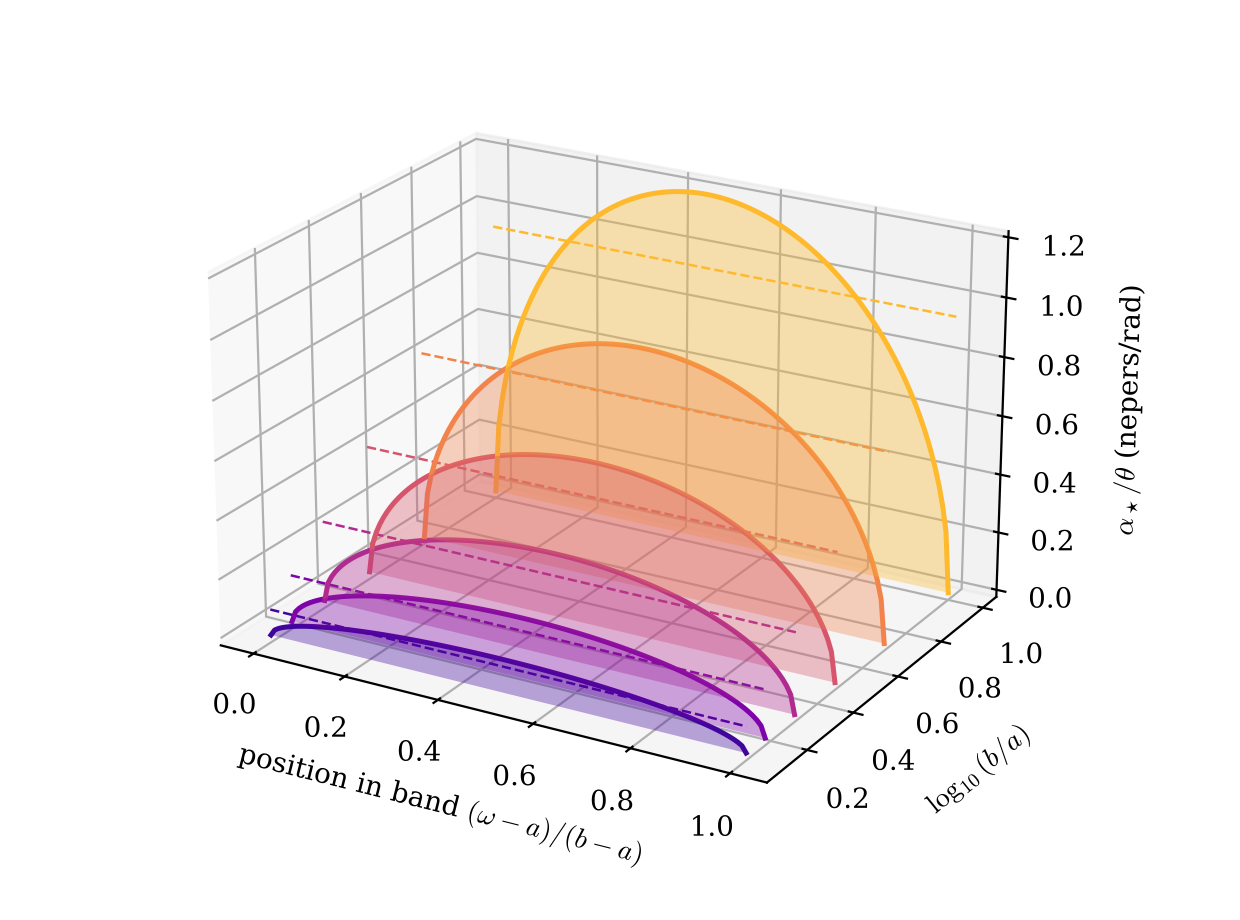
\includegraphics[width=\columnwidth]{figures/fig_extremal.png}
\caption{The attenuation $\alpha_\star/\theta$ of the extremal system across
the band, for $b/a=1.25,1.5,2,3,5,10$. Dashed lines mark the mean,
$\Lambda$. The profile vanishes at both edges.}
\label{fig:extremal}
\end{figure}

\subsection{Extremal systems for other phases}

The construction extends to phases that are not constant, and this is what
we need for systems with zeros.

\begin{proposition}\label{prop:profile}
Let $g$ be continuously differentiable on $[a,b]$ and put
\begin{gather*}
h_g(z)=\frac{2zR(z)}\pi\int_a^b\frac{g(t)}{r(t)\,(z^2-t^2)}\dd t,\\
\beta_g=\frac2\pi\int_a^b\frac{g(t)}{r(t)}\dd t .
\end{gather*}
\begin{enumerate}
\item[(i)] $h_g$ is analytic in $\C\setminus S$, odd, real on
$\R\setminus S$, continuous up to $S$ from both sides, and
$h_g(z)=\beta_gz+O(z^{-1})$ at infinity.
\item[(ii)] For $a<x<b$, $\Re h_g(x+i0)=g(x)$ and
\[
\Im h_g(x+i0)=v_g(x)=\frac{2x\,r(x)}\pi\PV\int_a^b\frac{g(t)}{r(t)\,(x^2-t^2)}\dd t .
\]
\item[(iii)] If $v_g\ge0$ on $(a,b)$ and $\beta_g\ge0$, then $e^{ih_g}$ is a
zero-free passive system, regular on the band, with phase $g$ and
attenuation $v_g$ on the band and no measure outside $S$, so that
$\int_a^bv_g=\frac12\int_a^bg\,p$.
\item[(iv)] For constant $g=\theta$, $h_g=h_\star$.
\end{enumerate}
\end{proposition}

\begin{proof}
(i) The Cauchy integral $q(z)=\int_a^bg(t)\,(r(t)(z^2-t^2))^{-1}\dd t$ is
analytic off $S$ and even; $zR(z)q(z)$ is odd and real on $\R\setminus S$
because $R$ is real there (\cref{lem:R}). The density $g/r$ has
singularities of order $\abs{t-a}^{-1/2}$, $\abs{t-b}^{-1/2}$ at the ends, so
$q$ is $O(\abs{z-a}^{-1/2})$, $O(\abs{z-b}^{-1/2})$ there and H\"older
continuous up to the open cut \cite[Ch.~4]{muskhelishvili}; multiplied by
$R$, which vanishes like the square root, the product is continuous up to
$S$. At infinity $q(z)=z^{-2}\int_a^bg/r+O(z^{-4})$ and
$zR(z)=z^3(1+O(z^{-2}))$, which gives the expansion.
(ii) Write $2z/(z^2-t^2)=1/(z-t)+1/(z+t)$. By the Plemelj formula, at
$x+i0$ with $a<x<b$ the first part of $q$ contributes
$\PV\int g\,(r(t)(x-t))^{-1}\dd t-i\pi g(x)/r(x)$, so
\[
\frac2\pi xq(x+i0)=\frac{2x}\pi\PV\int_a^b\frac{g(t)\dd t}{r(t)(x^2-t^2)}-\frac{ig(x)}{r(x)} .
\]
Multiplying by $R(x+i0)=ir(x)$ gives the real part $g(x)$ and the imaginary
part $v_g(x)$.
(iii) As in the proof of \cref{thm:extremal}(iii), $\Im(h_g-\beta_gz)$ is
harmonic, continuous up to the axis, zero on $\R\setminus S$, equal to
$v_g\ge0$ on $S$, and tends to $0$ at infinity; so $\Im h_g\ge\beta_g\Im
z\ge0$. The last identity is \cref{thm:sumrule}.
(iv) Let $d=h_g-h_\star$. Both functions have real part $\theta$ on the upper
side of $(a,b)$, are real on $\R\setminus S$ and satisfy $h(\bar
z)=\overline{h(z)}$, so on the lower side the real part is again $\theta$ and
$d(x\pm i0)=\pm i\,e(x)$ with $e$ real and continuous. Since $R(x\pm i0)=\pm
ir(x)$, the function $d/R$ has the same boundary values $e/r$ from both
sides of $(a,b)$, and likewise on $(-b,-a)$. It is therefore analytic across
the open cuts, by Morera's theorem, and its singularities at $\pm a,\pm b$
are $O(\abs{z-c}^{-1/2})$, hence removable. So $d/R$ is entire. Both
functions have the linear term $\tau_\star z$, because
$\beta_\theta=2\theta I_0/\pi=\tau_\star$, so $d=O(z^{-1})$ and $d/R\to0$ at
infinity. Thus $d=0$.
\end{proof}

\begin{lemma}\label{lem:positivity}
If $g(t)/t$ is nonincreasing on $[a,b]$, then $v_g\ge0$. In particular
this holds when $g>0$ and $g$ is nonincreasing, and then also $\beta_g>0$.
\end{lemma}

\begin{proof}
Substitute $\sigma=t^2$ and write $G(\sigma)=g(\sqrt\sigma)/\sqrt\sigma$,
which is nonincreasing. Then
\[
\frac{g(t)\dd t}{r(t)}=\frac{G(\sigma)\dd\sigma}{2\sqrt{(\sigma-a^2)(b^2-\sigma)}},
\]
and with $\sigma_0=x^2$,
\begin{multline*}
v_g(x)=\frac{x\,r(x)}\pi\\
\times\PV\int_{a^2}^{b^2}\frac{G(\sigma)}{(\sigma_0-\sigma)
\sqrt{(\sigma-a^2)(b^2-\sigma)}}\dd\sigma .
\end{multline*}
Glauert's integral \cite{king},
\[
\PV\int_{A}^{B}\frac{\dd\sigma}{(\sigma_0-\sigma)\sqrt{(\sigma-A)(B-\sigma)}}=0
\]
for $A<\sigma_0<B$,
which follows from the substitution $\sigma=\frac{A+B}2-\frac{B-A}2\cos\phi$
and $\PV\int_0^\pi\dd\phi/(\cos\phi-\cos\phi_0)=0$, allows us to subtract
$G(\sigma_0)$:
\[
v_g(x)=\frac{x\,r(x)}\pi\int_{a^2}^{b^2}\frac{G(\sigma)-G(\sigma_0)}{\sigma_0-\sigma}
\frac{\dd\sigma}{\sqrt{(\sigma-a^2)(b^2-\sigma)}} .
\]
For a nonincreasing $G$ the difference quotient is nonnegative, so
$v_g\ge0$. If $g>0$ is nonincreasing, $g/t$ is decreasing, and $\beta_g>0$
is clear.
\end{proof}

\section{Pointwise bounds without zeros}\label{sec:pointwise}

The sum rule bounds a mean. For zero-free systems with an affine phase on
the band there is a stronger statement: one explicit system has the least
attenuation at every frequency of the band at once. The proof writes every
admissible $h$ as the function $h_g$ of \cref{prop:profile} plus terms, one
for each unit of measure off the band, each of which raises the attenuation
at every point of the band.\footnote{The decomposition is the sum rule of
\cref{sec:sumrule} read pointwise: the weight $W$ of \cref{lem:kernel} is
replaced by the kernels $k_0$, $k_t$ of \cref{lem:atoms}, which are positive
at every point of the band.}

Throughout, $\Sigma=(0,a)\cup(b,\infty)$ is the part of the positive axis
off the band, and $\mu_0=\mu(\{0\})$. Put
\begin{gather*}
\tau_\circ=\frac{2K(k)}{\pi b}=\frac{\tau_\star}\theta,\qquad
h_\circ=\frac{h_\star}\theta,\qquad A=\frac{\alpha_\star}\theta,
\end{gather*}
so that $h_\circ$ is the extremal function of \cref{thm:extremal} for
$\theta=1$, with linear coefficient $\tau_\circ$ and attenuation
$A(x)=\tau_\circ\int_a^x(m^2-s^2)\dd s/r(s)$ on the band.

\subsection{One unit of measure off the band}

For $t\in\Sigma$ and $a<x<b$ put
\begin{gather*}
K_0(z)=\frac{R(z)}{abz},\qquad
K_t(z)=\frac{2zR(z)}{R(t)\,(t^2-z^2)},\\
k_0(x)=\frac{r(x)}{abx},\qquad
k_t(x)=\frac{2x\,r(x)}{R(t)\,(t^2-x^2)} .
\end{gather*}
By \cref{lem:R}, $R(t)$ and $t^2-x^2$ have the same sign for $t\in\Sigma$,
so $k_0>0$ and $k_t>0$ on $(a,b)$.

\begin{lemma}\label{lem:atoms}
$K_0$ and $K_t$, $t\in\Sigma$, are odd, analytic in $\C\setminus(S\cup\{0,\pm t\})$,
real on $\R\setminus S$ away from their poles, and
\begin{align*}
K_0(z)&=\frac z{ab}-\frac1z+\frac1\pi\int_a^b\frac{2z\,k_0(s)}{s^2-z^2}\dd s,\\
K_t(z)&=-\frac{2z}{R(t)}+\frac{2z}{t^2-z^2}
+\frac1\pi\int_a^b\frac{2z\,k_t(s)}{s^2-z^2}\dd s .
\end{align*}
On the band $\Re K_0(x+i0)=\Re K_t(x+i0)=0$, $\Im K_0(x+i0)=k_0(x)$ and
$\Im K_t(x+i0)=k_t(x)$.
\end{lemma}

\begin{proof}
The parity and reality follow from \cref{lem:R}, and the boundary values on
the band from $R(x+i0)=ir(x)$. Call $D$ the difference of the two sides of
either identity. At infinity $R(z)=z^2+O(1)$, so $K_0=z/(ab)+O(z^{-1})$ and
$K_t=-2z/R(t)+O(z^{-1})$, and the Cauchy integrals are $O(z^{-1})$; hence
$D=O(z^{-1})$. At $z=0$, $R(0)=-ab$, so $K_0=-1/z+O(z)$. At $z=\pm t$ the
residue of $K_t$ is $-1$, as is that of $2z/(t^2-z^2)$. So $D$ is analytic
off $S$. The Cauchy integral of the density $k/\pi$, $k=k_0$ or $k_t$,
which is H\"older continuous inside the band and of order $\abs{s-c}^{1/2}$
at its ends $c$, has the boundary imaginary part $k$ on $(a,b)$ by the
Plemelj formula, as in the proof of \cref{prop:profile}(ii), and is
continuous up to $S$ \cite[Ch.~4]{muskhelishvili}. Both sides of each
identity have imaginary part $k$ on the upper side of the band, so $D$ is
real there, and by the symmetry $D(\bar z)=\overline{D(z)}$ it takes the same
values from below. So $D$ has no jump across the open band, and by oddness none across $(-b,-a)$; it is bounded near
$\pm a,\pm b$, hence entire, and it tends to $0$. Thus $D=0$.
\end{proof}

\subsection{The reconstruction}

\begin{theorem}\label{thm:reconstruction}
Let $H=\sigma e^{ih}$ be a zero-free passive system, regular on the band,
whose phase $g=\varphi$ is continuously differentiable on $[a,b]$. Then
$\int_\Sigma\dd\mu(t)/\abs{R(t)}<\infty$ and
\begin{equation}\label{eq:reconstruction}
h=h_g+\mu_0K_0+\int_\Sigma K_t\dd\mu(t).
\end{equation}
Consequently, for $a<x<b$,
\begin{gather}
\alpha(x)=v_g(x)+\mu_0\,k_0(x)+\int_\Sigma k_t(x)\dd\mu(t),\label{eq:positive}\\
\beta=\beta_g+\frac{\mu_0}{ab}-\int_\Sigma\frac{2\dd\mu(t)}{R(t)} .\label{eq:betarec}
\end{gather}
\end{theorem}

The first identity says that the attenuation on the band is the
attenuation $v_g$ forced by the phase alone, plus a strictly positive
contribution of every unit of measure off the band. The second shows the
price of that measure in another currency: mass at frequencies below the
band, where $R<0$, raises the linear coefficient, and mass above the band
lowers it.

\begin{proof}
\emph{Finiteness.} For $t\to\infty$, $\abs{R(t)}\sim t^2$, and
$\int\dd\mu/(1+t^2)<\infty$. Near $a$ and $b$ the measure has a bounded
density by \cref{lem:regular}, and $\abs{R}^{-1}$ has singularities of
order $\abs{t-a}^{-1/2}$, $\abs{t-b}^{-1/2}$. Near $0$, $\abs R\ge ab/2$.

\emph{The right side.} Call it $\hat h$. Since $\abs{K_t(z)}$ is bounded by
a constant times $\abs{R(t)}^{-1}$ for $t\in\Sigma$ and $z$ in a compact set
at positive distance from $S\cup\{0\}\cup\operatorname{supp}\mu$, and for
$x$ in a compact subset of $(a,b)$ the same holds near $x+i0$, the integral
converges locally uniformly there; $\hat h$ is analytic off
$S\cup\{0\}\cup\operatorname{supp}\mu\cup-\operatorname{supp}\mu$ and
continuous up to the open band, where by \cref{prop:profile}(ii) and
\cref{lem:atoms} its real part is $g$. Integrating the identities of
\cref{lem:atoms} against $\mu$, by Fubini's theorem since every term is
absolutely integrable,
\[
\hat h(z)=\hat\beta z-\frac{\mu_0}z+\int_\Sigma\frac{2z}{t^2-z^2}\dd\mu(t)
+\frac1\pi\int_a^b\frac{2z\,\hat v(s)}{s^2-z^2}\dd s ,
\]
with $\hat\beta$ the right side of \eqref{eq:betarec} and $\hat v$ that of
\eqref{eq:positive}. Here we used that $h_g=\beta_gz+\frac1\pi\int_a^b
2zv_g(s)\dd s/(s^2-z^2)$: the difference of the two sides is odd, analytic
off $S$, $O(z^{-1})$ at infinity, continuous up to $S$, and has no jump
across the band, so it is entire and vanishes.

\emph{$\hat v$ is bounded.} $v_g$ is continuous on $[a,b]$ by
\cref{prop:profile}(i). In $\hat v(x)$ only the mass of $\mu$ near the band
edges can produce a singularity. For $x=a+\varepsilon$ and $t=a-u$ with
$0<u<\delta$, $k_t(x)$ is at most a constant times
$\sqrt\varepsilon/(\sqrt u\,(u+\varepsilon))$, and the density of $\mu$ is
bounded there, while
\[
\sqrt\varepsilon\int_0^\delta\frac{\dd u}{\sqrt u\,(u+\varepsilon)}\le\pi;
\]
the edge $b$ is the same. The rest of $\mu$ contributes a bounded amount by
the finiteness above.

\emph{Uniqueness.} By \eqref{eq:foster} and \cref{lem:regular},
$h=\beta z-\mu_0/z+\int_\Sigma2z\dd\mu/(t^2-z^2)+\frac1\pi\int_a^b2z\alpha(s)
\dd s/(s^2-z^2)$. So
\[
q=h-\hat h=(\beta-\hat\beta)z+\frac1\pi\int_a^b\frac{2z\,(\alpha-\hat v)(s)}{s^2-z^2}\dd s ,
\]
which is analytic off $S$, odd, $O(z)$ at infinity, and $O(\log\abs{z-c})$
near each end $c$ of $S$, because $\alpha-\hat v$ is bounded. Both $h$ and
$\hat h$ are continuous up to the open band with real part $g$, so, exactly
as in the proof of \cref{prop:profile}(iv), $q/R$ has the same boundary
values from both sides of $(a,b)$ and of $(-b,-a)$. It is therefore analytic
across the open cuts, its singularities at $\pm a,\pm b$ are
$o(\abs{z-c}^{-1})$ and hence removable, and $q/R$ is entire. At infinity
$q/R=O(z^{-1})$. Hence $q=0$, which is \eqref{eq:reconstruction}; comparing
linear coefficients and densities gives $\beta=\hat\beta$ and
$\alpha=\hat v$ almost everywhere, hence everywhere by continuity.
\end{proof}

\begin{corollary}\label{cor:compare}
Under the hypotheses of \cref{thm:reconstruction}, for $a<x<b$,
\[
\alpha(x)\ \ge\ v_g(x)+\frac{r(x)}x\,\max\{0,-\beta_g\}.
\]
\end{corollary}

\begin{proof}
For $0<t<a<x$, $x/(x^2-t^2)>1/x$, so $k_t(x)>2r(x)/(x\abs{R(t)})$. Put
\[
C_{\rm in}=\frac{\mu_0}{ab}+\int_{(0,a)}\frac{2\dd\mu(t)}{\abs{R(t)}},\qquad
C_{\rm out}=\int_{(b,\infty)}\frac{2\dd\mu(t)}{R(t)} ,
\]
both nonnegative. By \eqref{eq:positive},
$\alpha(x)\ge v_g(x)+\frac{r(x)}xC_{\rm in}+\int_{(b,\infty)}k_t(x)\dd\mu(t)$,
and by \eqref{eq:betarec} and $\beta\ge0$,
$C_{\rm in}\ge C_{\rm out}-\beta_g\ge-\beta_g$.
\end{proof}

\subsection{Affine phase}

For $g(t)=t$, \cref{prop:profile} gives $\beta_g=\frac2\pi\int_a^bt\dd t/r(t)=1$
and $v_g=0$, by the substitution $\sigma=t^2$ and Glauert's integral (proof
of \cref{lem:positivity}); hence $h_g=z$. By linearity and
\cref{prop:profile}(iv), the phase $\theta+\tau\omega$ has
\begin{equation}\label{eq:affinehg}
h_g=\theta h_\circ+\tau z,\qquad v_g=\theta A,\qquad \beta_g=\theta\tau_\circ+\tau .
\end{equation}
The function $R(z)/z=abK_0(z)$ has, by \cref{lem:atoms}, linear coefficient
$1$, an atom $ab$ at the origin and band attenuation $r(x)/x$.

\begin{theorem}\label{thm:affine}
Let $\theta\ge0$, $\tau\in\R$, and $C=\max\{0,-\theta\tau_\circ-\tau\}$. Every
zero-free passive system, regular on the band, with phase $\theta+\tau\omega$
on $(a,b)$ satisfies
\begin{equation}\label{eq:affinebound}
\alpha(x)\ \ge\ \theta A(x)+C\,\frac{r(x)}x\qquad(a\le x\le b).
\end{equation}
Equality holds throughout the band for
\[
h_{\rm opt}(z)=\theta h_\circ(z)+\tau z+C\,\frac{R(z)}z ,
\]
and equality at a single point of $(a,b)$ forces $h=h_{\rm opt}$.
\end{theorem}

\begin{proof}
The bound is \cref{cor:compare} with \eqref{eq:affinehg}, extended to the
ends by continuity. By \cref{lem:atoms} and \eqref{eq:affinehg},
$h_{\rm opt}$ has the form \eqref{eq:foster} with linear coefficient
$\theta\tau_\circ+\tau+C\ge0$, an atom $Cab\ge0$ at the origin, and the
measure $\pi^{-1}(\theta A+Cr/x)\dd x\ge0$ on the band and nothing else. So
it is a Herglotz function with the symmetry of \eqref{eq:Hh}, continuous up
to a neighbourhood of $[a,b]$, and $e^{ih_{\rm opt}}$ is admissible with
phase $\theta+\tau\omega$ and attenuation $\theta A+Cr/x$.

Suppose equality at $x_0\in(a,b)$. In the proof of \cref{cor:compare} each
inequality is then an equality at $x_0$. Since $k_t(x_0)>0$ for $t>b$, $\mu$
vanishes on $(b,\infty)$; since the comparison for $0<t<a$ is strict, $\mu$
vanishes on $(0,a)$; and $C_{\rm in}=\mu_0/(ab)$ equals $C$. By
\eqref{eq:reconstruction}, $h=\theta h_\circ+\tau z+CabK_0=h_{\rm opt}$.
\end{proof}

\begin{figure}[t]
\centering
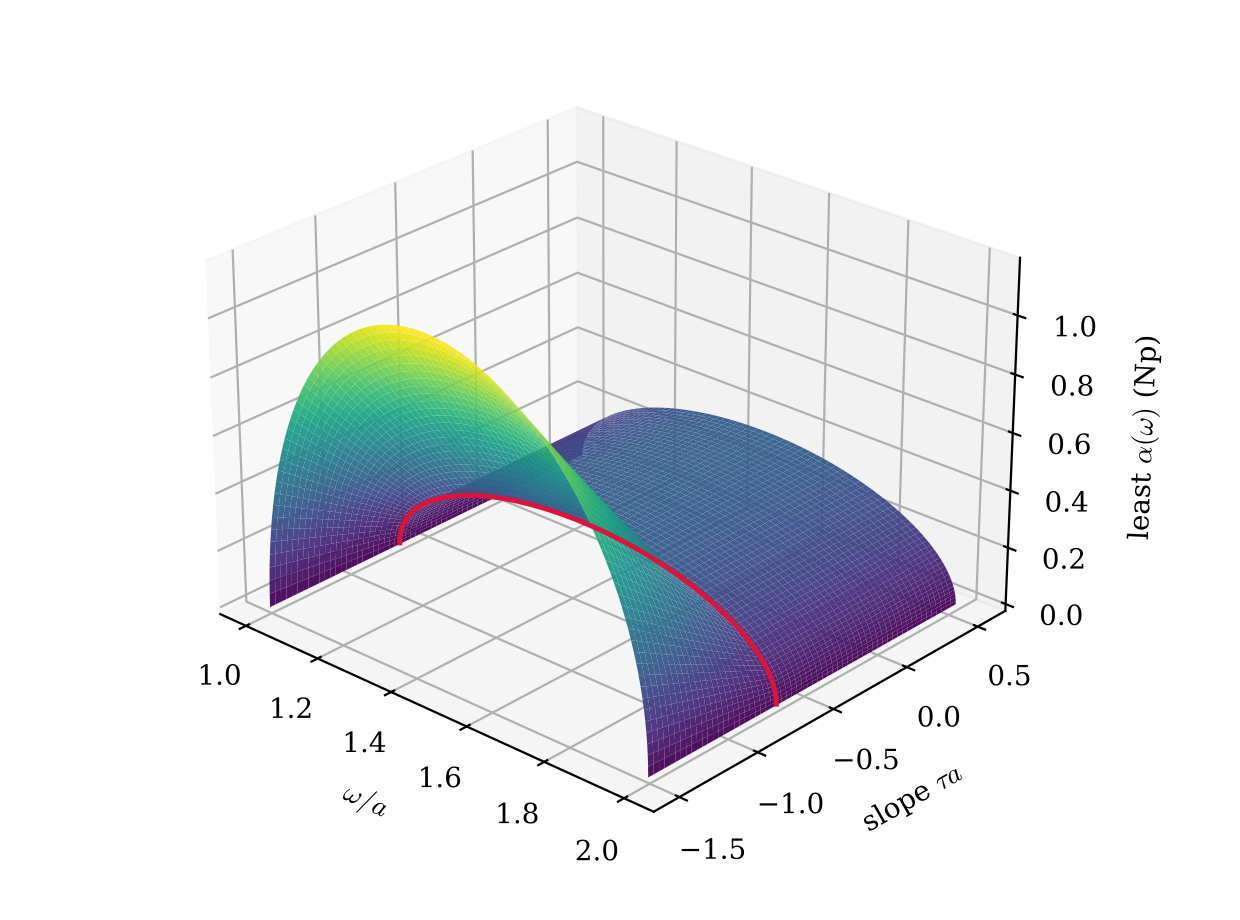
\includegraphics[width=\columnwidth]{figures/fig_pointwise.png}
\caption{The least attenuation $A(\omega)+\max\{0,-\tau_\circ-\tau\}\,r(\omega)/\omega$
of \cref{thm:affine} at each frequency of an octave, for the phase
$1+\tau\omega$, as a function of the slope $\tau$. For $\tau\ge-\tau_\circ$
(red curve at $\tau=-\tau_\circ=-0.6864/a$) it does not depend on $\tau$; below
it the pole at zero frequency adds $r(\omega)/\omega$ per unit of slope.}
\label{fig:pointwise}
\end{figure}

For $\tau\ge-\theta\tau_\circ$, in particular for a pure phase lag, the
optimum is $e^{i\tau z}H_\star$, and an additional delay costs nothing. A
negative slope beyond $-\theta\tau_\circ=-\tau_\star$ would make the linear
coefficient negative; the cheapest compensation, at every frequency of the
band at once, is then a pole of $h$ at zero frequency.

\subsection{Constant phase lead}

\begin{lemma}\label{lem:leadprofile}
$h_\circ(-ab/z)=-h_\circ(z)+\tau_\circ R(z)/z$. Consequently
\[
A(ab/x)=\tau_\circ\frac{r(x)}x-A(x)>0\qquad(a<x<b).
\]
\end{lemma}

\begin{proof}
The function $f(z)=h_\circ(-ab/z)$ is a Herglotz function with the symmetry
of \eqref{eq:Hh}, regular on the band, as in the proof of \cref{thm:lead};
its phase on the band is $-1$ and its attenuation is $A(ab/x)$. Since
$h_\circ$ is analytic at $0$ with $h_\circ(0)=0$, $f$ has linear coefficient
$0$; since $h_\circ(w)=\tau_\circ w+O(w^{-1})$, $f(z)=-\tau_\circ ab/z+O(z)$
near $0$, an atom $\tau_\circ ab$; and $f$ is real on $\Sigma$, so $\mu$ has
no other mass there. \Cref{thm:reconstruction} with $g=-1$, for which
$h_g=-h_\circ$, gives $f=-h_\circ+\tau_\circ abK_0$. Taking imaginary parts
on the band gives the second identity; $A(ab/x)>0$ by \cref{thm:extremal}(ii).
\end{proof}

\begin{theorem}\label{thm:leadpoint}
Let $s>0$ and $\tau\le0$. Every zero-free passive system, regular on the
band, with phase $-s+\tau\omega$ on $(a,b)$ satisfies
\[
\alpha(x)\ \ge\ s\,A(ab/x)-\tau\,\frac{r(x)}x\qquad(a\le x\le b),
\]
with equality throughout the band for
$h=-sh_\circ+\tau z+(s\tau_\circ-\tau)R/z$, and equality at one point of
$(a,b)$ forces this $h$. For $\tau=0$ the optimum is $H_\star(-ab/z)$ with
$H_\star$ the extremal system for $\theta=s$.
\end{theorem}

\begin{proof}
Here $v_g=-sA$ and $\beta_g=-s\tau_\circ+\tau<0$, so \cref{cor:compare} and
\cref{lem:leadprofile} give $\alpha\ge-sA+(s\tau_\circ-\tau)r/x
=sA(ab/x)-\tau r/x$. The stated $h$ has linear coefficient $0$, an atom
$(s\tau_\circ-\tau)ab>0$ at the origin and band density
$\pi^{-1}(sA(ab/x)-\tau r/x)>0$, so it is admissible. Equality at one point
forces $h$ as in the proof of \cref{thm:affine}. For $\tau=0$,
\cref{lem:leadprofile} identifies $h$ with $sh_\circ(-ab/z)$.
\end{proof}

\subsection{Consequences}

\begin{corollary}\label{cor:pointwisecons}
\begin{enumerate}
\item[(i)] For phase $\theta+\tau\omega$ with $\theta\ge0$, $\tau\in\R$, or
with $\theta<0$, $\tau\le0$, the optimal system of
\cref{thm:affine,thm:leadpoint} minimises $\int_a^bw\,\alpha$ for every
weight $w\ge0$, every $L^p$ norm of $\alpha$ on the band, $1\le p\le\infty$,
and every functional of $\alpha$ that increases with $\alpha$; for
$\int w\alpha$ with $w\ne0$ it is the only minimiser.
\item[(ii)] For phase $\theta\ge0$, the least value of $\max_{[a,b]}\alpha$ is
$\theta A(m)=\alpha_\star(m)$; for phase $-s<0$ it is $sA(m)$, attained at
$x=ab/m$.
\item[(iii)] For phase $-s<0$ the least mean attenuation over the band is
$s\Lambda_-$, with
\[
\Lambda_-=\frac{E(\kappa)-\kappa'^2K(\kappa)}{\kappa},\qquad\kappa'^2=1-\kappa^2 .
\]
\item[(iv)] For phase $\theta+\tau\omega$ with $\theta\ge0$ and
$\tau<-\tau_\star$, the least mean attenuation is
\[
\theta\Lambda+\frac\pi4\,(b-a)\,(-\tau-\tau_\star).
\]
\end{enumerate}
\end{corollary}

\begin{proof}
(i) follows from the pointwise bounds and their equality cases; a weight
$w\ge0$ that is not almost everywhere zero is positive on a set of positive
measure, where any other admissible system has strictly larger
attenuation, by the equality cases and continuity. (ii) $A$ is largest at
$m$ (\cref{thm:extremal}(ii)). (iii) is the value computed in
\cref{rem:leadmean} for $H_\star(-ab/z)$. (iv) Integrate
\eqref{eq:affinebound} with $C=-\tau-\tau_\star$, using
\[
\int_a^b\frac{r(x)}x\dd x=\frac\pi4(b-a)^2 ,
\]
which follows from $\sigma=x^2$, $A=a^2$, $B=b^2$ and the substitution
$\sigma=c-d\cos\phi$, $c=\frac{A+B}2$, $d=\frac{B-A}2$:
\begin{align*}
\int_A^B\frac{\sqrt{(\sigma-A)(B-\sigma)}}\sigma\dd\sigma
&=d^2\int_0^\pi\frac{\sin^2\phi\,\dd\phi}{c-d\cos\phi}\\
&=\pi\big(c-\sqrt{c^2-d^2}\big)\\
&=\frac\pi2\big(\sqrt B-\sqrt A\big)^2 ,
\end{align*}
since $c^2-d^2=AB$.
\end{proof}

For an octave $A(m)=0.34824$, so the least worst-frequency attenuation for a
lag $\theta$ is $1.2731\,\theta\Lambda$, against the mean $\theta\Lambda=0.27353\,\theta$;
and $\Lambda_-=0.26560$. So the sharp worst-frequency bound for a lag and the sharp plain mean for
a lead are both attained by the extremal system or by its inversion.

\begin{figure}[t]
\centering
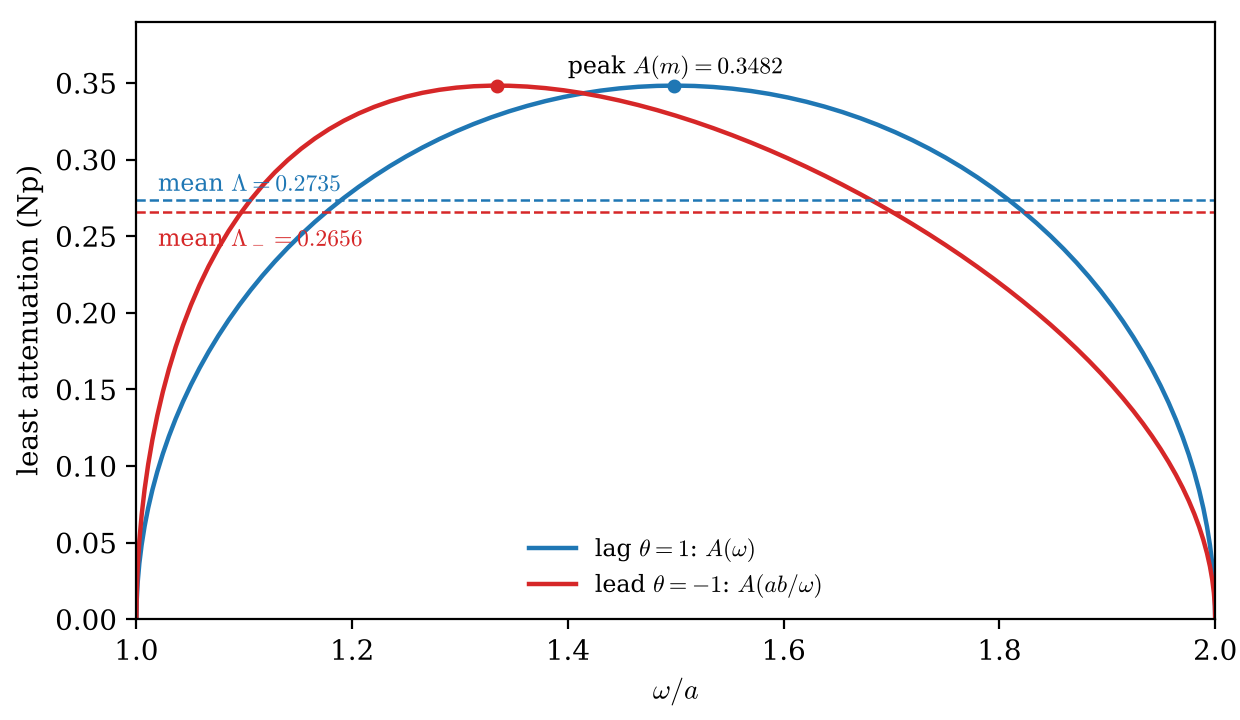
\includegraphics[width=\columnwidth]{figures/fig_leadlag.png}
\caption{The least attenuation at each frequency of an octave for a unit
lag (\cref{thm:affine}) and a unit lead (\cref{thm:leadpoint}). The lead
profile is the lag profile reflected by $\omega\mapsto ab/\omega$; the two
have the same peak $A(m)$, at $m$ and at $ab/m$, and different means.}
\label{fig:leadlag}
\end{figure}

\subsection{A prescribed argument}

\begin{theorem}\label{thm:branches}
Let $0<\vartheta<\pi$. Among zero-free passive systems regular on the band
with $\arg H\equiv\vartheta$ modulo $2\pi$ on $[a,b]$, the least mean
attenuation is $\min\{\vartheta\Lambda,(\pi-\vartheta)\Lambda_-\}$ and the
least value of $\max_{[a,b]}\alpha$ is $\min\{\vartheta,\pi-\vartheta\}A(m)$.
\end{theorem}

\begin{proof}
By \cref{rem:arg} the phase is a constant $\theta'\equiv\vartheta\pmod\pi$.
If $\theta'>0$ then $\theta'\ge\vartheta$, and by \cref{thm:main} and
\cref{cor:pointwisecons}(ii) both costs are at least $\vartheta\Lambda$ and
$\vartheta A(m)$, with equality for $H_\star$ with $\theta=\vartheta$. If
$\theta'<0$ then $\abs{\theta'}\ge\pi-\vartheta$, and
\cref{cor:pointwisecons}(ii), (iii) give $(\pi-\vartheta)\Lambda_-$ and
$(\pi-\vartheta)A(m)$, attained by $-H_\star(-ab/z)$ with $\theta=\pi-\vartheta$.
\end{proof}

So the mean is least on the lagging branch for
$\vartheta<\vartheta_c=\pi\Lambda_-/(\Lambda+\Lambda_-)$ and on the leading
branch beyond it, while the worst frequency changes branch at $\pi/2$. For an
octave $\vartheta_c=1.5477$, just below $\pi/2$: the two costs prefer
different systems for $\vartheta_c<\vartheta<\pi/2$. \Cref{thm:branches}
sharpens \cref{cor:worst}, whose constant $\Lambda$ becomes $A(m)$.

\section{Systems with zeros}\label{sec:zeros}

The main theorem concerns zero-free systems. A passive system may also have
zeros in $\Cp$, and a zero contributes phase without contributing loss on
the real axis. This section shows that zeros do help, and by how much one
zero helps.

\subsection{The bound with an inner factor}

\begin{proposition}\label{prop:inner}
Let $H=BG$ be passive, where $B$ is a real-symmetric Blaschke product whose
zeros stay away from $I\cup(-I)$ and $G$ is zero-free and regular on the
band. Let $\varphi$ be a continuous argument of $H$ on $[a,b]$ and let $\psi$
be the continuous argument of $B$ on $[a,b]$ for which $\varphi-\psi$ is the
phase of $G$ in the sense of \cref{lem:log}. Then $\alpha=\alpha_G$ on the
band, and
\begin{equation}\label{eq:inner}
\begin{aligned}
\int_a^b\alpha\dd\omega&=\frac12\int_a^b(\varphi-\psi)\,p\dd\omega
+\frac\pi4\int_{\R\setminus S}W\dd\mu_G\\
&\ge\ \frac12\int_a^b(\varphi-\psi)\,p\dd\omega .
\end{aligned}
\end{equation}
The function $\psi$ is real-analytic and strictly increasing on $[a,b]$.
\end{proposition}

\begin{proof}
The Blaschke product is analytic across $I$ and unimodular there, so
$\log\abs H=\log\abs G$ on the band, and $\arg H=\arg B+\arg G$ modulo $2\pi$.
The continuous arguments on $[a,b]$ therefore differ by a constant in
$2\pi\Z$, which fixes $\psi$. \Cref{thm:sumrule} applied to $G$ gives
\eqref{eq:inner}. The monotonicity of $\psi$ is the computation in the
proof of \cref{prop:foster}.\footnote{For a single factor
$(z-\zeta)/(z-\bar\zeta)$ with $\zeta=\xi+i\eta$, $\eta>0$, the argument on the
real line is $\arg(x-\zeta)-\arg(x-\bar\zeta)$, and
$\frac{\dd}{\dd x}\arg(x-\xi\mp i\eta)=\pm\eta/((x-\xi)^2+\eta^2)$; the
difference is $2\eta/\abs{x-\zeta}^2$.}
\end{proof}

An increasing $\psi$ behaves like a delay distributed over frequency. A pure
delay is free (\cref{lem:moments}(i)), but a phase that rises steeply at low
frequencies and flattens on the band is not a delay: its weighted integral
$\int\psi p$ is positive, and \eqref{eq:inner} then allows less loss than
\eqref{eq:main}. The simplest instance is a single zero on the imaginary
axis.

\subsection{One zero}

For $\eta>0$ let
\[
B_\eta(z)=\frac{z-i\eta}{z+i\eta}.
\]
It is passive, unimodular on $\R$, has the real symmetry, and the argument
of $-B_\eta$ on $(0,\infty)$ is
\begin{equation}\label{eq:Bphase}
\arg\big(-B_\eta(\omega)\big)=\pi-2\arctan\frac\eta\omega=2\arctan\frac\omega\eta
\in(0,\pi).
\end{equation}
For $0<\theta<\pi$ put $\eta_\theta=b\cot(\theta/2)$, so that
$2\arctan(b/\eta_\theta)=\theta$.

\begin{proposition}\label{prop:onezero}
Let $0<\theta<\pi$ and $\eta\ge\eta_\theta$, and put
\[
g_\eta(\omega)=\theta-2\arctan\frac\omega\eta,\qquad
H_\eta=-B_\eta\,e^{ih_{g_\eta}},
\]
with $h_g$ as in \cref{prop:profile}. Then $H_\eta$ is passive and regular on
the band, has exactly one zero in $\Cp$, at $i\eta$, has argument $\theta$
on $[a,b]$, and
\begin{equation}\label{eq:onezero}
\begin{gathered}
\frac1{b-a}\int_a^b\alpha_\eta\dd\omega=\theta\Lambda-\delta(\eta),\\
\delta(\eta)=\frac1{b-a}\int_a^b\arctan\frac\omega\eta\,p(\omega)\dd\omega .
\end{gathered}
\end{equation}
The reduction $\delta$ is strictly positive and strictly decreasing in $\eta$,
and
\begin{equation}\label{eq:delta-asym}
\delta(\eta)=\frac{\pi(b^2-a^2)^2}{24(b-a)\eta^3}+O(\eta^{-5})\qquad(\eta\to\infty).
\end{equation}
\end{proposition}

\begin{proof}
On $[a,b]$ the function $g_\eta$ is decreasing, and $g_\eta(b)\ge0$ because
$\eta\ge\eta_\theta$. Hence $g_\eta\ge0$, $g_\eta>0$ on $[a,b)$, and
$g_\eta(t)/t$ is decreasing. By \cref{lem:positivity}, $v_{g_\eta}\ge0$ and
$\beta_{g_\eta}>0$, so by \cref{prop:profile}(iii) $e^{ih_{g_\eta}}$ is a
zero-free passive system, regular on the band, with phase $g_\eta$ and
attenuation $v_{g_\eta}$, and with no measure outside $S$. Multiplying by
$-B_\eta$ keeps passivity and the real symmetry, adds the single zero $i\eta$,
leaves the modulus on $\R$ unchanged, and adds the argument
\eqref{eq:Bphase}. The argument of $H_\eta$ on the band is therefore
$g_\eta+2\arctan(\omega/\eta)=\theta$, and \cref{prop:profile}(iii) gives
\[
\int_a^b\alpha_\eta=\frac12\int_a^bg_\eta\,p=\frac\theta2J-\int_a^b\arctan\frac\omega\eta\,p\dd\omega,
\]
which is \eqref{eq:onezero} since $J=2(b-a)\Lambda$.

For the sign, write $\arctan(x/\eta)=x\,f(x^2)$ with
$f(\sigma)=\arctan(\sqrt\sigma/\eta)/\sqrt\sigma$. Since $u\mapsto\arctan(u)/u$
is strictly decreasing on $(0,\infty)$,\footnote{Its derivative is
$\big(u/(1+u^2)-\arctan u\big)/u^2$, and $\arctan u>u/(1+u^2)$ for $u>0$ because
both vanish at $0$ and $\frac{\dd}{\dd u}\arctan u=\frac1{1+u^2}>
\frac{1-u^2}{(1+u^2)^2}=\frac{\dd}{\dd u}\frac u{1+u^2}$.} $f$ is strictly
decreasing, and \cref{lem:moments}(ii) gives $\delta(\eta)>0$. Similarly
\[
\delta'(\eta)=-\frac1{b-a}\int_a^b\frac{x\,p(x)}{\eta^2+x^2}\dd x<0,
\]
by \cref{lem:moments}(ii) with the strictly decreasing
$f(\sigma)=1/(\eta^2+\sigma)$. Finally
$\arctan u=u-u^3/3+O(u^5)$ uniformly on $[0,b/\eta]$, and
\cref{lem:moments}(i),(iv) give $\int_a^bx\,p=0$ and
$\int_a^bx^3p=-\frac\pi8(b^2-a^2)^2$, which yields \eqref{eq:delta-asym}.
\end{proof}

Since $\delta$ decreases, the best choice within the family is
$\eta=\eta_\theta$, where the phase $g_\eta$ of the zero-free factor reaches
zero at the upper band edge. \Cref{fig:zero} shows the mean loss of
$H_\eta$, relative to $\theta\Lambda$, over $\theta$ and $\eta/\eta_\theta$.

\begin{figure}[t]
\centering
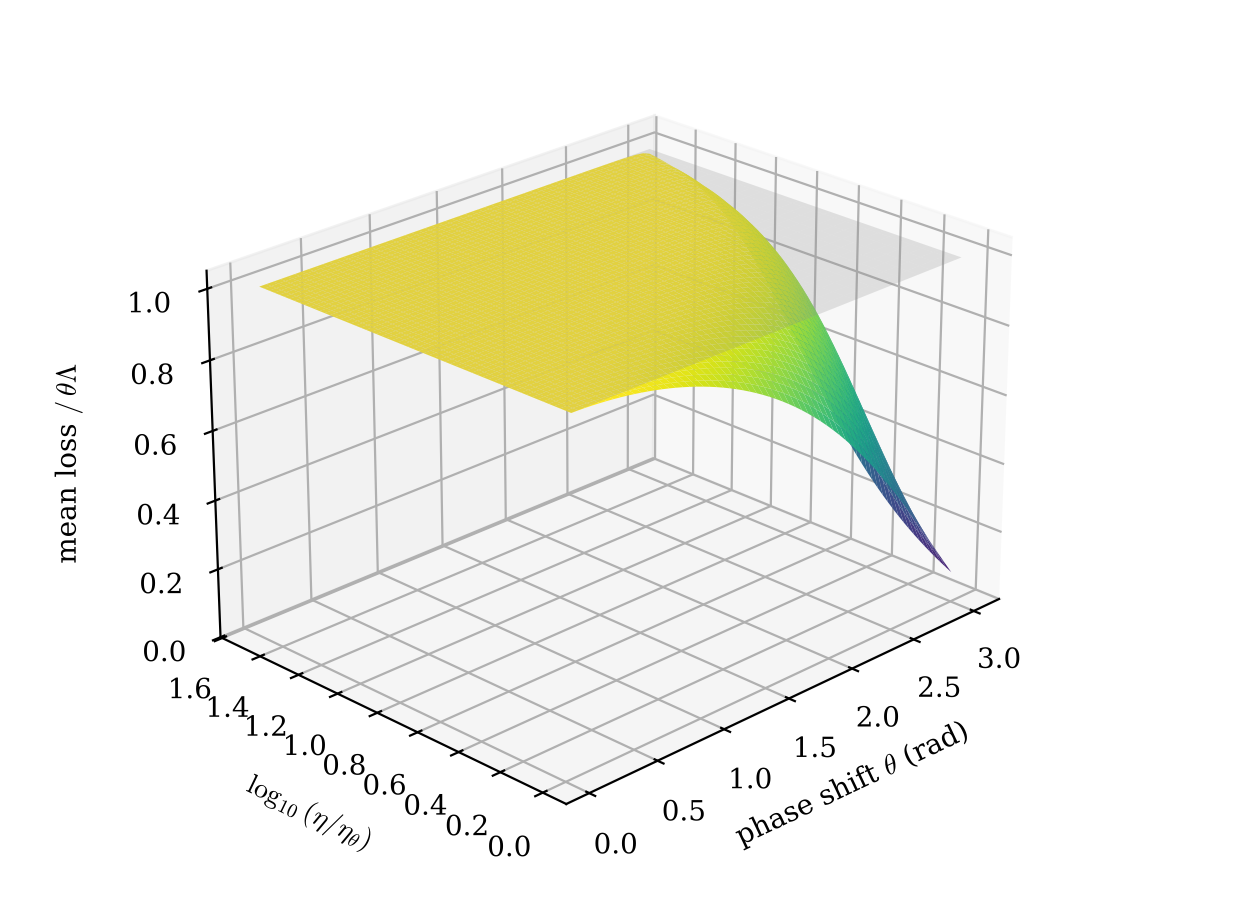
\includegraphics[width=\columnwidth]{figures/fig_zero.png}
\caption{The mean attenuation of the one-zero system $H_\eta$ of
\cref{prop:onezero}, divided by the zero-free bound $\theta\Lambda$, for
$a=1$, $b=2$, over the phase $\theta$ and $\log_{10}(\eta/\eta_\theta)$. The
grey plane is the level $1$. The ratio is below $1$ everywhere and tends to
$1$ as the zero moves to infinity.}
\label{fig:zero}
\end{figure}

\subsection{One zero beats every zero-free system}

The statement of \cref{thm:main} fixes the continuous phase $\varphi$. A
measurement only gives the argument modulo $2\pi$, and a zero-free system
with $\arg H\equiv\theta$ may realise $\theta$ through a lead $\theta-\pi$, by
\cref{rem:arg}. The next corollary takes this into account.

\begin{corollary}\label{cor:zerosbeat}
Let $0<\theta<a\pi/(a+b)$. Among zero-free passive systems regular on the
band with $\arg H\equiv\theta$ modulo $2\pi$ on $[a,b]$, the least mean
attenuation over the band is $\theta\Lambda$, attained by $H_\star$. The
system $H_{\eta_\theta}$ of \cref{prop:onezero}, which has one zero, has the
same argument and a strictly smaller mean attenuation.
\end{corollary}

\begin{proof}
By \cref{rem:arg} the phase of such a system is a constant $\theta'$ with
$\theta'\equiv\theta\pmod\pi$. If $\theta'\ge\theta$, \cref{thm:main} gives
mean attenuation at least $\theta'\Lambda\ge\theta\Lambda$. Otherwise
$\theta'\le\theta-\pi<0$, and \cref{thm:lead} with $\tau=0$ bounds the
$ab/\omega^2$-weighted mean by $\abs{\theta'}\Lambda\ge(\pi-\theta)\Lambda$.
Since $ab/\omega^2\le b/a$ on $[a,b]$, the plain mean is at least
$(a/b)(\pi-\theta)\Lambda$, which exceeds $\theta\Lambda$ exactly when
$\theta<a\pi/(a+b)$. The value $\theta\Lambda$ is attained by $H_\star$
(\cref{thm:extremal}), and \cref{prop:onezero} gives the second statement.
\end{proof}

For larger $\theta$ the lead branch competes. The system
$-H_\star(-ab/z)$, built from the extremal for $\pi-\theta$, is zero-free, has
$\sigma=-1$ and phase $\theta-\pi$, hence argument $\theta$ modulo $2\pi$, and
by \cref{rem:leadmean} its mean attenuation is
$(\pi-\theta)\,(E(\kappa)-\kappa'^2K(\kappa))/\kappa$. \Cref{tab:zeros} compares the
three systems for an octave.

\begin{table}[t]
\caption{Mean attenuation over the octave $[1,2]$ of three systems with
argument $\theta$ modulo $2\pi$: the lag extremal $H_\star$ (the least value
among zero-free systems with phase $\theta$), the lead extremal
$-H_\star(-ab/z)$ built for $\pi-\theta$, and the one-zero system
$H_{\eta_\theta}$. For $\theta<\pi/3$ the first column is the least value
among all zero-free systems (\cref{cor:zerosbeat}).}
\label{tab:zeros}
\centering
\small
\begin{tabular}{@{}rrrr@{}}
\toprule
$\theta$ & $\theta\Lambda$ & $(\pi-\theta)\,0.26560$ & $H_{\eta_\theta}$ \\
\midrule
$0.5$    & $0.13677$ & $0.70160$ & $0.13443$ \\
$1$      & $0.27353$ & $0.56880$ & $0.25394$ \\
$\pi/2$  & $0.42966$ & $0.41720$ & $0.34659$ \\
$2$      & $0.54707$ & $0.30320$ & $0.35977$ \\
$2.5$    & $0.68383$ & $0.17040$ & $0.27677$ \\
\bottomrule
\end{tabular}
\end{table}

The one-zero system is the best of the three for $\theta\le\pi/2$; by
$\theta=2$ the lead branch is better. For $\theta=0.5$ the zero lowers
the loss by $1.7\%$, for $\theta=1$ by $7.2\%$.

\subsection{The problem}

\begin{problem}\label{prob:zeros}
Determine
\[
\Lambda_{\mathrm{all}}(\theta)=\inf\Big\{\frac1{b-a}\int_a^b\alpha\dd\omega\Big\},
\]
the infimum over all passive systems $H$, with or without zeros, that are
continuous and nonzero near the band and satisfy $\arg H\equiv\theta$ modulo
$2\pi$ on $[a,b]$. Is $\Lambda_{\mathrm{all}}(\theta)>0$ for
$\theta\notin\pi\Z$?
\end{problem}

\Cref{cor:rigid} shows that the infimum is not attained by a lossless
system, but it does not exclude that it is zero. By \eqref{eq:inner}, the
question is how large $\int_a^b\psi\,p$ can be made by the argument $\psi$ of
a Blaschke product, while the remaining phase $\theta-\psi$ is still the
phase of a zero-free passive system. The difficulty is the second
condition: by \cref{prop:profile} it requires $v_g\ge0$ and $\beta_g\ge0$ for
$g=\theta-\psi$, and $\beta_g\ge0$ fails as soon as $g$ is too negative on the
band.\footnote{For instance, two zeros chosen so that $g<0$ on the whole band
give $\beta_g=\frac2\pi\int g/r<0$; the resulting function $e^{ih_g}$ grows
like $e^{-\beta_g y}$ along $i\R_+$ and is not passive.} The next section
solves the problem. The infimum is positive and attained, the minimiser has
exactly one zero, and it is the least lossy system at every frequency of the
band at once.

\section{The least loss with zeros}\label{sec:allzeros}

This section solves \cref{prob:zeros}. The answer is stronger than the
problem asks. For every phase $\theta\notin\pi\Z$ there is one passive system
whose attenuation is the least possible at every frequency of the band
simultaneously, among all passive systems with that argument, with or
without zeros. It has exactly one zero, on the imaginary axis, and it is
lossless off the band. For $\theta=\pi/2$ it is algebraic, and every quantity
is elementary.

\subsection{Statement}

We call a passive system $H$ \emph{admissible for} $\theta$ if it is regular
on the band in the sense of \cref{def:band} (the definition makes sense for
any passive system) and $\arg H\equiv\theta\pmod{2\pi}$ on $[a,b]$. The
admissible systems are exactly those of \cref{prob:zeros}. Since $-H$ is
passive whenever $H$ is, and $\arg(-H)=\arg H+\pi$, it suffices to treat
$0<\theta<\pi$. We use $r$, $h_g$, $v_g$, $\beta_g$, $B_\eta$ and $\delta$ as in
\cref{sec:extremal,sec:zeros}.

\begin{theorem}\label{thm:allzeros}
Let $0<\theta<\pi$. The equation
\begin{equation}\label{eq:etastar}
\int_a^b\frac{2\arctan(t/\eta)}{r(t)}\dd t=\theta\int_a^b\frac{\dd t}{r(t)}
\end{equation}
has exactly one root $\eta_\star\in(0,\eta_\theta)$. Put
\begin{gather*}
g_\sharp(\omega)=\theta-2\arctan\frac\omega{\eta_\star},\qquad
\Hs_\theta=-B_{\eta_\star}e^{ih_{g_\sharp}},\\
\as_\theta=v_{g_\sharp}\quad\text{on }[a,b].
\end{gather*}
\begin{enumerate}
\item[(i)] $\Hs_\theta$ is admissible for $\theta$. It has exactly one zero in
$\Cp$, at $i\eta_\star$, it is lossless on $\R\setminus S$, it satisfies
$\Hs_\theta(0)=1$ and $\Hs_\theta(iy)\to-1$ as $y\to\infty$, and its
attenuation $\as_\theta$ is positive on $(a,b)$ and vanishes at $a$ and $b$.
\item[(ii)] Every system $H$ admissible for $\theta$ satisfies
\begin{equation}\label{eq:pointwise}
\alpha(\omega)\ge\as_\theta(\omega)\qquad(a\le\omega\le b).
\end{equation}
If equality holds on a set of positive measure, then $H=\Hs_\theta$.
\item[(iii)] Consequently
\begin{equation}\label{eq:lambdaall}
\Lambda_{\mathrm{all}}(\theta)=\frac1{b-a}\int_a^b\as_\theta\dd\omega
=\theta\Lambda-\delta(\eta_\star)>0,
\end{equation}
the infimum is attained only by $\Hs_\theta$, and it is strictly smaller than
the mean attenuation of every system of \cref{prop:onezero}. For
$\pi<\theta<2\pi$, $\Lambda_{\mathrm{all}}(\theta)=\Lambda_{\mathrm{all}}(\theta-\pi)$,
attained only by $-\Hs_{\theta-\pi}$.
\end{enumerate}
\end{theorem}

The inequality \eqref{eq:pointwise} is pointwise. A single system is
optimal for the mean, for every weighted mean, for the worst frequency and
for the geometric mean at the same time (\cref{cor:allweights}). The
zero-free theory has the same feature for an affine phase
(\cref{thm:affine}), although its sum rule bounds only the mean; there the
constraint $\beta\ge0$ ties the frequencies of the band together, and
zeros remove it (\cref{rem:whypointwise}).

For a right angle everything is explicit.

\begin{theorem}\label{thm:rightangle}
Let $\theta=\pi/2$. Then $\eta_\star=\sqrt{ab}$, and
\begin{equation}\label{eq:Hright}
\Hs_{\pi/2}(z)=-\frac{z^2+ab}{R(z)+i(a+b)z},
\end{equation}
with $R$ as in \cref{lem:R}. Its attenuation is
\begin{equation}\label{eq:alpharight}
\begin{aligned}
\as_{\pi/2}(\omega)&=\log\frac{(a+b)\,\omega+r(\omega)}{\omega^2+ab}\\
&=2\operatorname{artanh}\sqrt{\frac{(\omega-a)(b-\omega)}{(\omega+a)(\omega+b)}} ,
\end{aligned}
\end{equation}
and
\begin{equation}\label{eq:lambdaright}
\int_a^b\as_{\pi/2}\dd\omega=\frac\pi2\big(\sqrt b-\sqrt a\big)^2,\quad
\Lambda_{\mathrm{all}}\Big(\frac\pi2\Big)=\frac\pi2\,\frac{\sqrt b-\sqrt a}{\sqrt b+\sqrt a}.
\end{equation}
The profile $\as_{\pi/2}$ is invariant under $\omega\mapsto ab/\omega$ and has
its only maximum at the geometric centre $\omega_0=\sqrt{ab}$, where
$\as_{\pi/2}(\omega_0)=\frac12\log(b/a)$. Hence every passive system with
$\arg H\equiv\pi/2\pmod\pi$ on $[a,b]$ that is regular on the band satisfies
\begin{equation}\label{eq:threedb}
\abs{H(\omega)}\le\frac{\omega^2+ab}{(a+b)\,\omega+r(\omega)},\qquad
\abs{H(\sqrt{ab})}^2\le\frac ab .
\end{equation}
\end{theorem}

For an octave, a passive system whose phase is a right angle at every
frequency of the band transmits at most half of the power at the geometric
centre: its loss there is at least $3.01$\,dB, and for a decade at least
$10$\,dB.\footnote{The power transmission is $\abs H^2\le a/b$, so the loss
is at least $10\log_{10}(b/a)$\,dB: $10\log_{10}2=3.0103$ and
$10\log_{10}10=10$.} The sum rule of the zero-free theory gives no bound of
this pointwise kind. The mean attenuation of
$\Hs_{\pi/2}$ over an octave is $\frac\pi2(3-2\sqrt2)=0.26951$\,Np, which is
$62.7\%$ of the zero-free value $\frac\pi2\Lambda=0.42966$. For a narrow band
the ratio of the two minimal means tends to $\sin\theta/\theta$
(\cref{cor:narrowzeros}), which is $2/\pi$ at a right angle.

\begin{table}[t]
\caption{The least mean attenuation over the octave $[1,2]$ of passive
systems with argument $\theta$ modulo $2\pi$, with or without zeros
(\cref{thm:allzeros}), the position of the zero of the optimal system
relative to $\eta_\theta=b\cot(\theta/2)$ of \cref{prop:onezero}, the ratio to
the zero-free value $\theta\Lambda$, and the least possible worst-frequency
attenuation $\max\as_\theta$.}
\label{tab:allzeros}
\centering
\small
\begin{tabular}{@{}rrrrr@{}}
\toprule
$\theta$ & $\eta_\star/\eta_\theta$ & $\Lambda_{\mathrm{all}}(\theta)$ &
$\Lambda_{\mathrm{all}}/\theta\Lambda$ & $\max\as_\theta$ \\
\midrule
$0.5$    & $0.72576$ & $0.13090$ & $0.9571$ & $0.16677$ \\
$1$      & $0.71853$ & $0.22860$ & $0.8357$ & $0.29204$ \\
$\pi/2$  & $0.70711$ & $0.26951$ & $0.6272$ & $0.34657$ \\
$2$      & $0.69843$ & $0.24357$ & $0.4452$ & $0.31540$ \\
$2.5$    & $0.69050$ & $0.15941$ & $0.2331$ & $0.20805$ \\
\bottomrule
\end{tabular}
\end{table}

\Cref{tab:allzeros} gives the octave values, and \cref{fig:allzeros} the
optimal profiles. Comparing with \cref{tab:zeros}: the optimal system beats
the one-zero system $H_{\eta_\theta}$ for every $\theta$, by $2.6\%$ at
$\theta=0.5$ and $22\%$ at $\theta=\pi/2$, and for $\theta\ge2$ it also beats
the lead branch. Its zero sits closer to the origin than $\eta_\theta$, so that
the phase $g_\sharp$ of its zero-free factor is negative on part of the band,
which \cref{lem:positivity} does not allow. At $\theta=\pi/2$ the ratio
$\eta_\star/\eta_\theta$ is $\sqrt{a/b}$, by \cref{thm:rightangle}.

\begin{figure}[t]
\centering
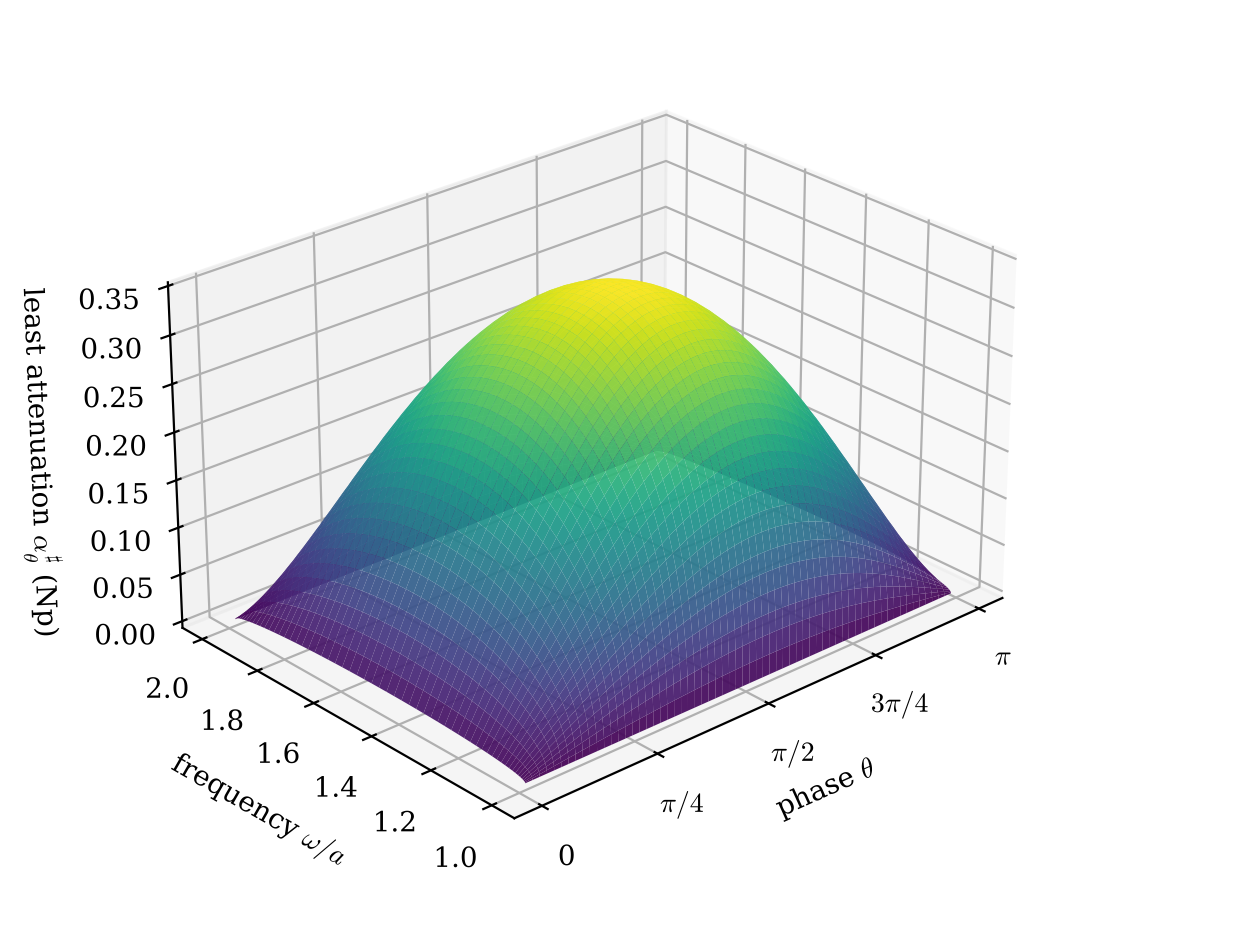
\includegraphics[width=\columnwidth]{figures/fig_allzeros.png}
\caption{The least attenuation $\as_\theta(\omega)$ at each frequency of the
octave, over the phase $\theta\in(0,\pi)$ (\cref{thm:allzeros}). No passive
system with argument $\theta$ on the band lies below the surface at any
frequency. The black curve is the closed form \eqref{eq:alpharight} at
$\theta=\pi/2$, with its peak $\frac12\log2$ at $\omega=\sqrt2$.}
\label{fig:allzeros}
\end{figure}

\begin{figure}[t]
\centering
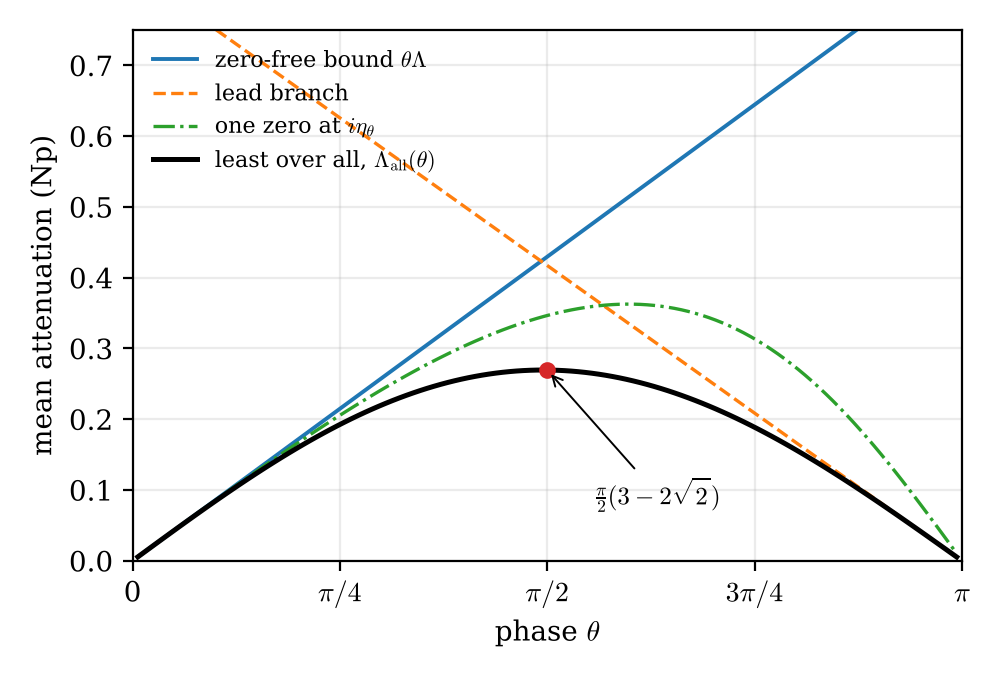
\includegraphics[width=\columnwidth]{figures/fig_lambdaall.png}
\caption{Mean attenuation over the octave against the phase $\theta$: the
zero-free bound $\theta\Lambda$ (\cref{thm:main}), the lead branch of
\cref{tab:zeros}, the one-zero system $H_{\eta_\theta}$
(\cref{prop:onezero}), and the exact minimum $\Lambda_{\mathrm{all}}(\theta)$
over all passive systems (\cref{thm:allzeros}). The dot marks the closed form
$\frac\pi2(3-2\sqrt2)$ at $\theta=\pi/2$.}
\label{fig:lambdaall}
\end{figure}

\subsection{A change of variables}

The phase condition $\arg H\equiv\theta$ is not linear in $\log H$ once
zeros are allowed, since $\log H$ is then not defined. A M\"obius
transformation of the values removes this difficulty.

\begin{lemma}\label{lem:transform}
Let $0<\theta<\pi$, let $H$ be a passive system that is not constant, and
put
\begin{equation}\label{eq:F}
F=e^{-i\theta}\,\frac{H-e^{i\theta}}{H-e^{-i\theta}},\qquad
H=\frac{F-e^{i\theta}}{e^{i\theta}F-1}.
\end{equation}
\begin{enumerate}
\item[(i)] $F$ is analytic in $\Cp$ with values in $\Cp$, and
$F(-\bar z)=1/\overline{F(z)}$. The function $\zeta=\log F$, with
$0<\Im\zeta<\pi$, satisfies $\zeta(-\bar z)=-\overline{\zeta(z)}$, and
\begin{equation}\label{eq:zetarep}
\zeta(z)=\frac1\pi\int_0^\infty g(t)\,\frac{2z}{t^2-z^2}\dd t ,
\end{equation}
where $g(t)=\Im\zeta(t+i0)\in[0,\pi]$ for almost every $t>0$. In
particular $\Re\zeta=0$ on $i\R_+$.
\item[(ii)] Conversely, if $F$ is analytic in $\Cp$ with values in $\Cp$ and
$F(-\bar z)=1/\overline{F(z)}$, then \eqref{eq:F} defines a passive system.
\item[(iii)] $\abs H=1$ at a point $t\in\R$ where $H$ is continuous if and
only if $F(t)$ is real there, and then $g(t)\in\{0,\pi\}$. The zeros of $H$
are the points where $F=e^{i\theta}$.
\item[(iv)] Let $H(\omega)=e^{i\theta-\alpha}$ with $\alpha>0$ at a point
$\omega$ of the band, and write $\zeta=u+iv$ there. (If $\alpha=0$, then $F=0$.)
Then
\begin{equation}\label{eq:bandcurve}
\frac1F=\cos\theta-i\sin\theta\coth\frac\alpha2,\qquad
e^u\cos\theta=\cos v,
\end{equation}
$u<0$, $v$ lies strictly between $\theta$ and $\pi/2$ (or $v=\pi/2$ if
$\theta=\pi/2$), and
\begin{equation}\label{eq:Au}
\alpha=A_\theta(u),\qquad
A_\theta(u)=2\operatorname{artanh}\frac{e^u\sin\theta}{\sqrt{1-e^{2u}\cos^2\theta}},
\end{equation}
where $A_\theta$ is a strictly increasing bijection of $(-\infty,0)$ onto
$(0,\infty)$. Conversely, a value $1/F$ of the form \eqref{eq:bandcurve}
with $\alpha>0$ corresponds to $H=e^{i\theta-\alpha}$.
\end{enumerate}
\end{lemma}

\begin{proof}
(i) Since $H$ is not constant, $\abs H<1$ in $\Cp$ by the maximum principle,
so $H\ne e^{\pm i\theta}$ there. The M\"obius map
$w\mapsto e^{-i\theta}(w-e^{i\theta})/(w-e^{-i\theta})$ sends the unit circle into
the real line\footnote{For $w=e^{i\phi}$,
$e^{i\phi}-e^{i\theta}=2ie^{i(\phi+\theta)/2}\sin\frac{\phi-\theta}2$ and
$e^{i\phi}-e^{-i\theta}=2ie^{i(\phi-\theta)/2}\sin\frac{\phi+\theta}2$, so the
image is $\sin\frac{\phi-\theta}2/\sin\frac{\phi+\theta}2\in\R$.} and $0$ to
$e^{i\theta}\in\Cp$, so it maps the open disc onto $\Cp$. The symmetry
$H(-\bar z)=\overline{H(z)}$ gives
$F(-\bar z)=e^{-i\theta}(\bar H-e^{i\theta})/(\bar H-e^{-i\theta})
=1/\overline{F(z)}$, hence the symmetry of $\zeta$. The function $\zeta$ is a
Herglotz function with bounded imaginary part, so in \eqref{eq:herglotz}
$\beta=0$ and $\dd\mu=\pi^{-1}g\dd t$ with $g$ the boundary values of $\Im\zeta$
\cite[Ch.~I]{garnett}. On $i\R_+$ the symmetry reads $\zeta=-\bar\zeta$, so
$\Re\zeta=0$ there and $c=\Re\zeta(i)=0$. The symmetry also makes $g$ even,
and folding the integral over $\R$ onto $(0,\infty)$ with
$\frac1{t-z}-\frac1{-t-z}=\frac{2z}{t^2-z^2}$ gives \eqref{eq:zetarep}; the
terms $t/(1+t^2)$ cancel.
(ii) The inverse M\"obius map in \eqref{eq:F} sends $\Cp$ into the open unit
disc, and the symmetry of $H$ follows by reversing the computation in (i).
(iii) The M\"obius map sends the unit circle onto the real line, and
$H=0$ exactly when $F=e^{-i\theta}(-e^{i\theta})/(-e^{-i\theta})=e^{i\theta}$.
(iv) Substituting $H=e^{i\theta-\alpha}$ in $1/F=e^{i\theta}(H-e^{-i\theta})/(H-e^{i\theta})$
gives
\[
\frac1F=\frac{(e^{-\alpha}-1)\cos\theta+i(e^{-\alpha}+1)\sin\theta}{e^{-\alpha}-1},
\]
which is the first identity of \eqref{eq:bandcurve}. Since
$1/F=e^{-u}(\cos v-i\sin v)$, the real parts give $e^u\cos\theta=\cos v$, and
the imaginary parts $\tanh(\alpha/2)=e^u\sin\theta/\sin v$. As
$\coth(\alpha/2)>1$, $\abs{1/F}>1$, so $u<0$, and then $\abs{\cos v}<\abs{\cos\theta}$
with the same sign, which places $v$ between $\theta$ and $\pi/2$. Finally
$\sin v=\sqrt{1-e^{2u}\cos^2\theta}$ gives \eqref{eq:Au}. The quotient
$e^u\sin\theta/\sqrt{1-e^{2u}\cos^2\theta}$ increases with $u$, tends to $0$ as
$u\to-\infty$ and to $1$ as $u\to0$.
\end{proof}

So the band condition places the boundary value of $\zeta$ on the curve
\[
\Gamma_\theta=\{u+iv:\ u<0,\ e^u\cos\theta=\cos v\},
\]
with $v$ between $\theta$ and $\pi/2$, and the attenuation is an increasing
function of $u$ alone. Off the band, $g$ is free in $[0,\pi]$; a lossless
stretch has $g\in\{0,\pi\}$. In the variable $\zeta$ the zeros of $H$ have
disappeared.

\subsection{The comparison theorem}

We use two facts about Hardy spaces of the unit disc $\mathbb D$
\cite[Chs.~3,~4]{duren}. (a) If $f$ is analytic in $\mathbb D$ and
$\abs{\arg f}\le\lambda<\pi/2$, then $f\in H^q$ for every $q<\pi/(2\lambda)$; this
follows from the case $\lambda=\pi/2$, $q<1$, applied to $f^{\pi/(2\lambda)}$. (b)
If $\Im f$ is bounded, then $f\in H^p$ for every $p<\infty$, by the theorem of
M.~Riesz. A function in $H^1$ is the Poisson integral of its boundary
values, and so is its imaginary part. Through the Cayley map
$w=(z-i)/(z+i)$ these statements apply to functions in $\Cp$, and for $Y$ in
$H^1$ of the disc they give
\begin{equation}\label{eq:schwarzhalf}
Y(z)=\Re Y(i)+\frac1\pi\int_\R\Im Y(t)\Big(\frac1{t-z}-\frac t{1+t^2}\Big)\dd t ,
\end{equation}
with $\int\abs{Y(t)}\dd t/(1+t^2)<\infty$.\footnote{At $z=i$ the integral is
$\frac i\pi\int\Im Y(t)\dd t/(1+t^2)$, which is purely imaginary, so the real
constant is $\Re Y(i)$. The imaginary part of the kernel is the Poisson
kernel $y/((t-x)^2+y^2)$.}

\begin{proposition}\label{prop:compare}
Let $0<\theta<\pi$ and let $\Hs$ be admissible for $\theta$, with
\begin{equation}\label{eq:tight}
g_\sharp=\pi\ \text{on }(0,a),\qquad g_\sharp=0\ \text{on }(b,\infty)
\end{equation}
for the function $g_\sharp$ of \cref{lem:transform} belonging to $\Hs$. Then every
$H$ admissible for $\theta$ satisfies $\alpha\ge\as$ on $[a,b]$, where $\as$ is
the attenuation of $\Hs$. If $\alpha=\as$ on a set of positive measure, then
$H=\Hs$. In particular at most one admissible system satisfies
\eqref{eq:tight}.
\end{proposition}

\begin{proof}
Let $\zeta=u+iv$ and $\zeta_\sharp=u_\sharp+iv_\sharp$ be the functions of
\cref{lem:transform} for $H$ and $\Hs$, and $d=\zeta-\zeta_\sharp$. The function
$F$ of $H$ is continuous up to $(a,b)$, so $u=\log\abs F$ is continuous there
with values in $[-\infty,0)$, and $u=-\infty$ exactly on the closed set $Z$
where $H=e^{i\theta}$. Since $\Im\zeta$ is bounded, $\zeta$ has finite boundary
values almost everywhere (fact (b) above), so $Z$ has measure zero. The
attenuation $\as$ of $\Hs$ is positive on $(a,b)$, since $u_\sharp$ is finite
there, $\Hs$ being regular on the band. By \cref{lem:transform}(iv) it
suffices to show $u\ge u_\sharp$ almost everywhere on $(a,b)$: then, by
continuity, everywhere, so that $Z$ is empty and $\alpha=A_\theta(u)\ge
A_\theta(u_\sharp)=\as$.

\emph{Step 1: the chord.} The curve $\Gamma_\theta$ is the graph of
$V(u)=\arccos(e^u\cos\theta)$, and $V'(u)=-\cot V(u)$, where $\cot V$ has the sign
$\epsilon=\operatorname{sign}\cos\theta$ and $\abs{\cot V}\le\abs{\cot\theta}$ because
$V$ lies between $\theta$ and $\pi/2$. By the mean value theorem, at each
$x\in(a,b)\setminus Z$
\[
d(x)=\big(u(x)-u_\sharp(x)\big)\big(1-i\,m(x)\big)
\]
with $m(x)=\cot V(\xi)$ for some $\xi$ between $u(x)$ and $u_\sharp(x)$ (and $m=0$
where $u=u_\sharp$). Put $\psi=\arctan m$. Then $\abs\psi\le\lambda$, with
$\lambda=\abs{\pi/2-\theta}<\pi/2$, $\psi$ is measurable, and
$1-im=\sqrt{1+m^2}\,e^{-i\psi}$.

\emph{Step 2: a rotating factor.} Define
\[
\Xi(z)=\frac1\pi\int_a^b\psi(t)\,\frac{2t}{t^2-z^2}\dd t,\qquad X=e^\Xi .
\]
The density $\frac1\pi\psi(\abs t)\operatorname{sign}t$ on $S$ is bounded, so $\Im\Xi$
is its Poisson integral: $\abs{\Im\Xi}\le\lambda$ in $\Cp$, $\Im\Xi=\psi$ almost
everywhere on $(a,b)$, $\Im\Xi=0$ on $\R\setminus S$, and $\Xi(-\bar z)=\overline{\Xi(z)}$.
Hence $X$ is real and positive on $i\R_+$ and on $\R\setminus S$, $X\to1$ at
infinity, and $\abs{\arg X}\le\lambda$. If $\theta=\pi/2$, then $X\equiv1$.

\emph{Step 3: the product.} Let $Y=Xd$. By (a), $X\in H^q$ for some $q>1$; by
(b), $d\in H^p$ for every $p<\infty$, since $\abs{\Im d}\le\pi$. By H\"older's
inequality $Y\in H^1$. At almost every $x\in(a,b)$,
\begin{equation}\label{eq:Yband}
Y(x)=\abs{X(x)}\sqrt{1+m(x)^2}\,\big(u(x)-u_\sharp(x)\big)\in\R ,
\end{equation}
since the factor $e^{i\psi}$ of $X$ cancels $e^{-i\psi}$. On $\R\setminus S$,
$\Im Y=X\,(g-g_\sharp)$, which by \eqref{eq:tight} and $0\le g\le\pi$ is $\le0$
on $(0,a)$ and $\ge0$ on $(b,\infty)$. Both $X$ and $d$ have the symmetries
$X(-\bar z)=\overline{X(z)}$, $d(-\bar z)=-\overline{d(z)}$, so
$Y(-\bar z)=-\overline{Y(z)}$; thus $\Im Y$ is even on $\R$ and $Y$ is purely
imaginary on $i\R_+$, so that $\Re Y(i)=0$.

\emph{Step 4: the sign.} By \eqref{eq:schwarzhalf}, folded onto $(0,\infty)$
as in \cref{lem:transform}, and since $\Im Y=0$ on $(a,b)$,
\[
Y(z)=\frac1\pi\int_{(0,a)\cup(b,\infty)}\Im Y(t)\,\frac{2z}{t^2-z^2}\dd t .
\]
The right side is analytic across $(a,b)$, so for $a<x<b$
\begin{multline}\label{eq:Ysign}
Y(x)=\frac1\pi\int_0^a\big(-\Im Y(t)\big)\frac{2x}{x^2-t^2}\dd t\\
+\frac1\pi\int_b^\infty\Im Y(t)\,\frac{2x}{t^2-x^2}\dd t\ \ge\ 0 ,
\end{multline}
both integrands being nonnegative. With \eqref{eq:Yband} this gives
$u\ge u_\sharp$ almost everywhere on $(a,b)$.

\emph{Equality.} If $\alpha=\as$ on a set of positive measure, pick a point of
it at which \eqref{eq:Yband} holds. There $Y=0$, so both integrals in
\eqref{eq:Ysign} vanish, and since $X>0$ and the kernels do not vanish,
$g=g_\sharp$ almost everywhere off the band. Then $\Im Y=0$ almost
everywhere on $\R$, so $Y\equiv0$ by \eqref{eq:schwarzhalf}, hence $d\equiv0$
and $H=\Hs$.
\end{proof}

\begin{remark}\label{rem:whypointwise}
For zero-free systems the analogue of $\zeta$ is $ih$, and the constraint
$\Re h=\theta$ on the band is linear; there the coefficient $\beta\ge0$ of
the linear term of $h$ acts as a single global constraint, which
\cref{cor:compare} turns into a pointwise price $r(x)/x$ per unit of
$-\beta_g$. In the variable
$\zeta$ the linear term is absent, because $\Im\zeta$ is bounded, and the band
condition is a curve rather than a line. The proof above replaces linearity
by the observation that the chords of $\Gamma_\theta$ have slopes in a fixed
sector, which the factor $X$ rotates to the real axis. The constraint
$\beta\ge0$ is what zeros remove: in the factorisation
$\Hs_\theta=-B_{\eta_\star}e^{ih_{g_\sharp}}$ the zero-free factor has
$\beta_{g_\sharp}=0$ (\cref{lem:identify}).
\end{remark}

\subsection{The right angle}

\begin{proof}[Proof of \cref{thm:rightangle}]
Let $Q(z)=(z+a)(z+b)$ and
\[
\zeta_0(z)=\tfrac12\big(\log(z-a)+\log(z-b)-\log(z+a)-\log(z+b)\big)
\]
with the arguments in $(0,\pi)$. For $z\in\Cp$ the angle $\arg(z-c)-\arg(z+c)$
lies in $(0,\pi)$ for $c=a,b$,\footnote{It is the angle at $z$ of the
triangle with vertices $-c$, $c$, $z$.} so $0<\Im\zeta_0<\pi$. On $(0,a)$,
$\Im\zeta_0=\frac12(\pi+\pi)=\pi$; on $(b,\infty)$ it is $0$; on $(a,b)$ it is
$\pi/2$, and $\zeta_0(-\bar z)=-\overline{\zeta_0(z)}$. So $\zeta_0$ has the form
\eqref{eq:zetarep}, with $g_0=\pi$ on $(0,a)$, $\pi/2$ on $(a,b)$, $0$ on
$(b,\infty)$. Since $e^{2\zeta_0}=(z-a)(z-b)/Q(z)=R^2/Q^2$ and both $e^{\zeta_0}$
and $R/Q$ tend to $1$ at infinity, $F_0=e^{\zeta_0}=R/Q$. By
\cref{lem:transform}(ii), \eqref{eq:F} with $\theta=\pi/2$ defines a passive
system
\[
K=\frac{F_0-i}{iF_0-1}=\frac{R-iQ}{iR-Q}=-\frac{z^2+ab}{R+i(a+b)z},
\]
where the last step uses $R^2=(z^2-a^2)(z^2-b^2)$ and
$(z^2-a^2)(z^2-b^2)+(a+b)^2z^2=(z^2+ab)^2$.\footnote{Cross-multiplying,
$(R-iQ)(R+i(a+b)z)=R^2+(a+b)zQ-iR(z^2+ab)$, since $(a+b)z-Q=-(z^2+ab)$, while
$-(z^2+ab)(iR-Q)=(z^2+ab)Q-iR(z^2+ab)$, and $R^2=Q\,(z-a)(z-b)=Q(z^2+ab-(a+b)z)$.}
On the band $F_0=ir/Q$ is purely imaginary, so $\Re(1/F_0)=0=\cos(\pi/2)$ and,
by \eqref{eq:bandcurve}, $K=e^{i\pi/2-\alpha}$ with
$\tanh(\alpha/2)=e^{u}=r/Q$, which is the second form of \eqref{eq:alpharight}. The first form is
$\log\frac{1+s}{1-s}$ with $s=r/Q$, because
$(Q+r)(\omega^2+ab)=(Q-r)\big((a+b)\omega+r\big)$ on the band.\footnote{Write
$c=(a+b)\omega$ and $m=\omega^2+ab$, so $Q=m+c$. The two sides are $m^2+cm+rm$ and
$mc+mr+c^2-r^2$, and $c^2-m^2=(a^2+b^2)\omega^2-\omega^4-a^2b^2=r^2$.}
The system $K$ is regular on the band, with $K\to e^{i\pi/2}$ at the band
edges, and its function $g_0$ satisfies \eqref{eq:tight}. By
\cref{prop:compare}, $K$ is the unique admissible system with this property.
It has exactly one zero, a simple one at $i\sqrt{ab}$, where
$z^2+ab=0$ and $R+i(a+b)z=-2(a+b)\sqrt{ab}\ne0$;\footnote{On $i\R_+$,
$R(iy)=-\sqrt{(y^2+a^2)(y^2+b^2)}$, being real, nonvanishing and $\sim-y^2$.}
moreover $K(0)=-ab/R(0)=1$ and $K(iy)\to-1$. So \cref{lem:identify} below,
applied to $K$, gives $K=\Hs_{\pi/2}$ and $\eta_\star=\sqrt{ab}$. (Directly: the substitution $t=ab/s$ maps $\dd t/r(t)$
to $\dd s/r(s)$ and $\arctan(t/\sqrt{ab})$ to
$\frac\pi2-\arctan(s/\sqrt{ab})$, so the left side of \eqref{eq:etastar} at
$\eta=\sqrt{ab}$ is $\frac\pi2\int\dd t/r$.)

For \eqref{eq:lambdaright}, write $K=-B_{\sqrt{ab}}\,e^{ih}$, where
$h=h_{g_\sharp}$. By \cref{prop:profile}(iii) and \eqref{eq:foster},
\[
h(z)=\frac1\pi\int_a^b\as_{\pi/2}(t)\,\frac{2z}{t^2-z^2}\dd t ,
\]
so
\[
\lim_{y\to\infty}iy\,h(iy)=-\frac2\pi\int_a^b\as_{\pi/2}\dd t .
\]
On the other hand $R+i(a+b)z=z^2\big(1+i(a+b)/z+O(z^{-2})\big)$ and
$-B_\eta(z)=-1+2i\eta/z+O(z^{-2})$, so
\[
e^{ih}=\frac K{-B_{\sqrt{ab}}}=1-\frac{i\,(a+b-2\sqrt{ab})}z+O(z^{-2}),
\]
whence $zh(z)\to-(\sqrt b-\sqrt a)^2$, which is \eqref{eq:lambdaright}.

Finally, $q(\omega)=(\omega-a)(b-\omega)/((\omega+a)(\omega+b))$ satisfies
$q(ab/\omega)=q(\omega)$, and $\log q$ is strictly concave on $(a,b)$, since
$(\log q)''=\frac1{(\omega+a)^2}-\frac1{(\omega-a)^2}+\frac1{(\omega+b)^2}-\frac1{(b-\omega)^2}<0$.
So its only maximum is at the fixed point $\sqrt{ab}$, where
$\sqrt q=(\sqrt b-\sqrt a)/(\sqrt b+\sqrt a)$ and
$2\operatorname{artanh}\sqrt q=\log(\sqrt b/\sqrt a)$. The bound \eqref{eq:threedb}
is $\abs H=e^{-\alpha}\le e^{-\as_{\pi/2}}$, from \cref{thm:allzeros}(ii), applied to
$H$ or $-H$.
\end{proof}

\subsection{Existence for every phase}

For $\theta\ne\pi/2$ the optimal system is not algebraic, and we construct it
by a conformal map. In the variable $\sigma=z^2$, the first quadrant becomes
$\Cp$, and the boundary conditions of \cref{lem:transform} for a system with
\eqref{eq:tight} become conditions on $G=1/F$: $G$ is real and
below $-1$ on $(0,a^2)$, real and above $1$ on $(b^2,\infty)$, unimodular on
$(-\infty,0)$ (the imaginary axis of $z$, where $\Re\zeta=0$), and $\Re G=\cos\theta$
on $(a^2,b^2)$, by \eqref{eq:bandcurve}. This describes a slit domain
(\cref{fig:slitmap}).

\begin{figure}[t]
\centering
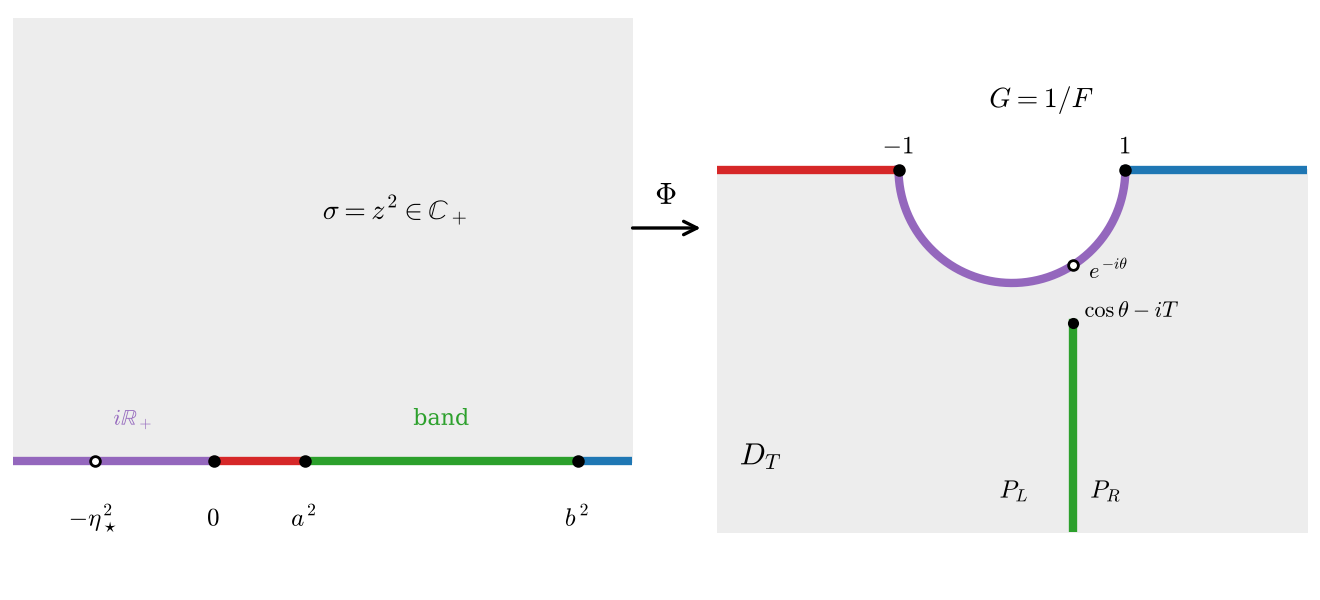
\includegraphics[width=\columnwidth]{figures/fig_slitmap.png}
\caption{The construction of \cref{prop:exist}. Left: the plane of
$\sigma=z^2$, with the boundary arcs coloured. Right: the domain $D_T$ of
$G=1/F$, the part of the lower half-plane outside the unit disc, cut along
the vertical ray $\Re G=\cos\theta$ below the tip $\cos\theta-iT$. The map
$\Phi$ sends each arc on the left to the arc of the same colour; the two ends
of the band go to the two ends of the slit at infinity. The zero of the
optimal system is the preimage of $e^{-i\theta}$.}
\label{fig:slitmap}
\end{figure}

\begin{proposition}\label{prop:exist}
Let $0<\theta<\pi$. There is a system $\Hs$, admissible for $\theta$, with
\eqref{eq:tight}, lossless on $\R\setminus S$, with exactly one zero in
$\Cp$, which is simple and lies on $i\R_+$, and with $\Hs(0)=1$,
$\Hs(iy)\to-1$ as $y\to\infty$, and attenuation positive on $(a,b)$ and zero
at $a$ and $b$.
\end{proposition}

\begin{proof}
For $T>\sin\theta$ let $\Sigma_T=\{\cos\theta-is:\ s\ge T\}$ and
\[
D_T=\{G:\ \Im G<0,\ \abs G>1\}\setminus\Sigma_T .
\]
The ray $\Sigma_T$ does not meet the closed unit disc, since
$\abs{\cos\theta-is}>1$ for $s>\sin\theta$. The domain $D_T$ is simply connected
and its boundary is locally connected, so a conformal map $\Phi$ of $\Cp$
onto $D_T$ extends to a homeomorphism of $\R\cup\{\infty\}$ onto the prime ends
of $D_T$ \cite[Ch.~2]{pommerenke}. Traversed with $D_T$ on the left, the
boundary consists of the lower unit semicircle $C$ from $1$ to $-1$, the ray
$(-\infty,-1]$, the left side of $\Sigma_T$ up to the tip and its right side
down again, and the ray $[1,\infty)$. It has two prime ends at infinity:
$P_L$, between $(-\infty,-1]$ and the left side of the slit, and $P_R$,
between the right side and $[1,\infty)$. We normalise $\Phi$ by $\Phi(\infty)=1$,
$\Phi(0)=-1$ and $\Phi(a^2)=P_L$, and let $s(T)>a^2$ be the preimage of $P_R$.

\emph{Choice of $T$.} Let $\lambda(T)$ be the extremal distance in $D_T$
between $C$ and $\Sigma_T$ \cite[Ch.~4]{ahlforsci}. By conformal invariance it
equals the extremal distance in $\Cp$ between $(-\infty,0)$ and $[a^2,s(T)]$,
which is $L(s(T)/a^2)$ for a continuous strictly decreasing bijection $L$ of
$(1,\infty)$ onto $(0,\infty)$.\footnote{By scaling, $L(\rho)$ is the extremal
distance between $(-\infty,0)$ and $[1,\rho]$. It decreases because the curve
family grows with $\rho$; it tends to $\infty$ as $\rho\to1$, since every curve
crosses the half-annulus $\rho-1<\abs{\sigma-1}<1$, of extremal distance
$\frac1\pi\log\frac1{\rho-1}$; and to $0$ as $\rho\to\infty$, since the half-circles
$\abs\sigma=t$, $1<t<\rho$, join the two sets and have length $\pi t$, which gives
modulus at least $\frac1\pi\log\rho$. Strictness and continuity follow from the
explicit value as a ratio of complete elliptic integrals.} The function
$\lambda$ is continuous in $T$: for $T'$ near $T$ a diffeomorphism
$G\mapsto G-i(T'-T)\chi(G)$, with $\chi$ a smooth bump equal to $1$ near the
tip and supported in a disc around it that avoids the unit circle and the
real axis, maps $D_T$ onto $D_{T'}$ arc by arc, with dilatation
$1+O(\abs{T'-T})$, and extremal distances change at most by that
factor.\footnote{It moves the slit along itself and fixes the rest of the
boundary; it is injective once $\abs{T'-T}\,\abs{\nabla\chi}<1$. A
diffeomorphism whose differential has ratio of singular values at most $K$
changes an extremal distance by a factor in $[1/K,K]$, by transporting the
admissible metrics \cite[Ch.~4]{ahlforsci}.} As $T\to\infty$, every curve in
$D_T$ from $C$ to $\Sigma_T$ crosses the annulus $1<\abs G<T$, so
$\lambda(T)\ge\frac1{2\pi}\log T\to\infty$. As $T\downarrow\sin\theta$, the tip
$\cos\theta-iT$ lies at the distance $\delta=T-\sin\theta$ below the point $e^{-i\theta}$
of $C$, and for $\delta<\rho<\rho_0$ an arc of the circle $\abs{G-e^{-i\theta}}=\rho$
of length less than $2\pi\rho$ joins $C$ to $\Sigma_T$ inside $D_T$; this gives
$\lambda(T)\le2\pi/\log(\rho_0/\delta)\to0$. Hence $s(T)/a^2$ is continuous and
takes every value in $(1,\infty)$, and we fix $T$ with $s(T)=b^2$.

\emph{The system.} On the open first quadrant put $F(z)=1/\Phi(z^2)$, and on
the open second quadrant $F(z)=1/\overline{F(-\bar z)}$. On $i\R_+$, $z^2<0$ is
mapped to $C$, where $\abs\Phi=1$, so the two definitions have the same
continuous boundary values there, and $F$ is analytic in $\Cp$ by Morera's
theorem. $F$ maps $\Cp$ into $\Cp$, since $\Im\Phi<0$, and
$F(-\bar z)=1/\overline{F(z)}$. Define $\Hs$ from $F$ by \eqref{eq:F}. By
\cref{lem:transform}(ii) it is a passive system. On $(0,a)$, $\Phi(t^2)<-1$,
so $F\in(-1,0)$ and $g_\sharp=\pi$; on $(b,\infty)$, $F\in(0,1)$ and $g_\sharp=0$;
in both cases $\abs\Hs=1$. On $(a,b)$, $\Phi(t^2)=\cos\theta-is$ with $s\ge T>\sin\theta$,
which by \eqref{eq:bandcurve} is $H=e^{i\theta-\alpha}$ with
$\coth(\alpha/2)=s/\sin\theta$, so $\alpha>0$, and $\alpha\to0$ at the band edges, where
$s\to\infty$, $F\to0$ and $\Hs\to e^{i\theta}$. Hence $\Hs$ is continuous and
nonzero on a neighbourhood of $[a,b]$, that is, regular on the band, with
argument $\theta$ there. By \cref{lem:transform}(iii) its zeros are the
points with $1/F=e^{-i\theta}$, a point of $C$; $\Phi$ takes this boundary value
at exactly one point of $(-\infty,0)$, and analytically, since $C$ is an
analytic arc, with nonzero derivative. So $\Hs$ has exactly one zero in
$\Cp$, a simple one on $i\R_+$. Finally $\Phi(0)=-1$ gives $F(0)=-1$ and
$\Hs(0)=1$, and $\Phi(\sigma)\to1$ as $\sigma\to-\infty$ gives $\Hs(iy)\to-1$.
\end{proof}

\begin{lemma}\label{lem:identify}
Let $\Hs$ be admissible for $\theta$, with \eqref{eq:tight}, lossless on
$\R\setminus S$, with exactly one zero in $\Cp$, a simple one at $i\eta$, and
with $\Hs(0)=1$ and $\Hs(iy)\to-1$ as $y\to\infty$; for instance the system of
\cref{prop:exist}. Then
$\Hs=-B_\eta e^{ih_g}$ with $g(\omega)=\theta-2\arctan(\omega/\eta)$, $\beta_g=0$, and
the attenuation of $\Hs$ on the band is $v_g$. Consequently $\eta$ is the
root $\eta_\star$ of \eqref{eq:etastar}.
\end{lemma}

\begin{proof}
The quotient $E=\Hs/(-B_\eta)$ is analytic and zero-free in $\Cp$, unimodular
where $\Hs$ is, and bounded, hence bounded by $1$ by the maximum principle, since
$\abs{B_\eta}\to1$ at $\R\cup\{\infty\}$. It has the real symmetry and
$E(0)=\Hs(0)/(-B_\eta(0))=1$, so by \cref{lem:log} $E=e^{ih}$ with an odd
Herglotz function $h$, $h(0)=0$. On $\R\setminus S$, $\abs E=1$, so $\Im h=0$ there:
the measure of $h$ is carried by $S$, and by \eqref{eq:herglotz}, $h$ being
odd, $h(z)=\beta z+O(z^{-1})$ at infinity. Along $[0,a]$ the function $F$ of
$\Hs$ is negative, by \eqref{eq:tight}, with $F(0)=-1$ and $F(a)=0$, so the
argument of $\Hs$ moves continuously from $0$ to $\theta$ inside
$(-\theta,\theta]$,\footnote{The inverse M\"obius map of \eqref{eq:F} sends
$(-\infty,0]$ to the arc of the unit circle from $e^{-i\theta}$ to $e^{i\theta}$
through $1$, with $-1\mapsto1$ and $0\mapsto e^{i\theta}$.} and that of $-B_\eta$ from $0$ to $2\arctan(a/\eta)$ by
\eqref{eq:Bphase}. So on the band $\Re h=\theta-2\arctan(\omega/\eta)=g$, with
no multiple of $2\pi$. The argument of \cref{prop:profile}(iv) now applies
to $h-h_g$: it is real on $\R\setminus S$, has real part $0$ on the band from
above, is continuous up to $S$ (since $E$ is continuous and nonzero near the
band), so $(h-h_g)/R$ is entire, and it is
$O(z^{-1})$ at infinity. Hence $h=h_g$ and $\beta=\beta_g$. Finally
$E(iy)\to(-1)/(-1)=1$, so $h(iy)\to0$ and $\beta=0$. The attenuation is
$\Im h_g=v_g$ on the band. The left side of \eqref{eq:etastar} decreases
strictly in $\eta$ from $\pi\int\dd t/r$ to $0$, so it has exactly one root,
and $\beta_g=0$ says that $\eta$ is this root.
\end{proof}

\begin{proof}[Proof of \cref{thm:allzeros}]
The system $\Hs_\theta=-B_{\eta_\star}e^{ih_{g_\sharp}}$ is the system of
\cref{prop:exist}, by \cref{lem:identify}. This gives (i), with $\as_\theta=v_{g_\sharp}>0$ on the
open band. Since $g_\sharp\ge0$ and decreasing for $\eta\ge\eta_\theta$,
$\beta_{g_\eta}>0$ there (\cref{lem:positivity}); and $\beta_{g_\eta}$ increases
with $\eta$; so $\eta_\star<\eta_\theta$. Part (ii) is \cref{prop:compare}. For
(iii), by \cref{prop:profile}(iii) with $v_{g_\sharp}\ge0$ and $\beta_{g_\sharp}=0$,
$\int_a^b\as_\theta=\frac12\int_a^bg_\sharp\,p$, and the computation in the proof of
\cref{prop:onezero} gives $\theta\Lambda-\delta(\eta_\star)$. It is positive since
$\as_\theta>0$. The systems $H_\eta$ of \cref{prop:onezero} are admissible and
differ from $\Hs_\theta$, since $\beta_{g_\eta}>0$, so by (ii) their mean is
strictly larger. The case $\pi<\theta<2\pi$ follows by passing to $-H$.
\end{proof}

\subsection{Consequences}

\begin{corollary}\label{cor:allweights}
Let $0<\theta<\pi$ and let $H$ be admissible for $\theta$.
\begin{enumerate}
\item[(i)] For every measurable $w\ge0$ on $[a,b]$,
$\int w\alpha\ge\int w\as_\theta$; in particular
$\max_{[a,b]}\alpha\ge\max_{[a,b]}\as_\theta$. The system $\Hs_\theta$ attains all of
these bounds at once.
\item[(ii)] A phase lead costs at least as much as no delay: if $H$ is
passive, regular on the band, and $\arg H\equiv\theta-\tau\omega\pmod{2\pi}$ on
$[a,b]$ for some $\tau\ge0$, then $\alpha\ge\as_\theta$ on $[a,b]$.
\item[(iii)] Every zero-free system with phase $\theta$ on the band, in the
sense of \cref{thm:main}, satisfies $\alpha\ge\as_\theta$ pointwise, in addition
to $\frac1{b-a}\int\alpha\ge\theta\Lambda$.
\end{enumerate}
\end{corollary}

\begin{proof}
(i) is \eqref{eq:pointwise}. (ii) The system $e^{i\tau z}H$ is passive, has
the same modulus on $\R$, and has argument $\theta$ on the band. (iii) is a
special case of (ii) with $\tau=0$.
\end{proof}

Part (i) answers, for systems with zeros allowed, the worst-frequency
question of the zero-free case. Part
(ii) does not extend to a delay, $\arg H=\theta+\tau\omega$ with $\tau>0$: the
system $e^{i\tau z}\Hs_\theta$ still has the loss $\as_\theta$, but it is not
optimal: for $\theta=\pi/2$, $\tau=5$ on $[1,2]$ the least mean loss of a
zero-free system is about forty times smaller (\cref{thm:delay,thm:exactmean}),
and with zeros the least loss falls exponentially in $\tau$ (\cref{cor:rate}).

\begin{corollary}\label{cor:narrowzeros}
Fix $0<\theta<\pi$, and let $f=(a+b)/2$, $\Delta f=b-a$. As $\Delta f/f\to0$,
\[
\Lambda_{\mathrm{all}}(\theta)=\frac\pi8\,\sin\theta\,\frac{\Delta f}f
+O\Big(\Big(\frac{\Delta f}f\Big)^2\Big),
\]
so that $\Lambda_{\mathrm{all}}(\theta)/\theta\Lambda\to\sin\theta/\theta$.
\end{corollary}

\begin{proof}
Write $\epsilon=\Delta f/f$. By \eqref{eq:intro-bounds}, $\Lambda=\frac\pi8\epsilon+O(\epsilon^3)$.
By the proof of \cref{prop:onezero}, $\int_a^bp=J=2(b-a)\Lambda$, and by
\cref{lem:moments}(i), $\int_a^b\omega p=0$, so
$\frac1{b-a}\int_a^b(\omega-f)p=-2f\Lambda$. Taylor's formula for
$\arctan(\omega/\eta)$ at $\omega=f$, with a remainder $O((\omega-f)^2/\eta^2)$ that
is integrated against $\abs p$, whose mean over the band is
$O(1)$,\footnote{In $\omega=f+\frac{\Delta f}2s$, $p\,\dd\omega/(b-a)=-s\,\dd s/\sqrt{1-s^2}\,(1+O(\epsilon))$.}
gives
\[
\delta(\eta)=2\Lambda\arctan\frac f\eta-2\Lambda\frac{f\eta}{f^2+\eta^2}
+O\Big(\frac{\epsilon^2f^2}{\eta^2}\Big).
\]
The root of \eqref{eq:etastar} satisfies $2\arctan(f/\eta_\star)=\theta+O(\epsilon)$,
since the weight $\dd t/r$ is carried by an interval of length $\epsilon f$
around $f$. With $\phi=2\arctan(f/\eta_\star)$ and
$2f\eta/(f^2+\eta^2)=\sin\phi$,
\begin{align*}
\Lambda_{\mathrm{all}}&=\theta\Lambda-\delta(\eta_\star)=\Lambda\,(\theta-\phi+\sin\phi)+O(\epsilon^2)\\
&=\Lambda\sin\theta+O(\epsilon^2),
\end{align*}
because $\Lambda=O(\epsilon)$ and $\theta-\phi=O(\epsilon)$; also $f/\eta_\star$ stays
bounded.
\end{proof}

In the computations (\cref{app:verification}) the relative error is of the
order of $(\Delta f/f)^2$: the ratio of $\Lambda_{\mathrm{all}}$ to the leading
term is $1.0021$ for $b/a=1.2$ and $1.000149$ for $b/a=1.05$ at $\theta=\pi/2$.
For small phases zeros hardly help: the gain is a factor
$\sin\theta/\theta=1-\theta^2/6+\dots$. For the $1^\circ$ shift at $5$\,MHz of
\cref{sec:waves}, the least mean attenuation with zeros allowed is
$1.37588\times10^{-3}$\,Np, against $1.37595\times10^{-3}$\,Np without zeros.

For general $\theta$ the profile $\as_\theta$ is elliptic, not elementary
(\cref{ssec:closedform}), and a simple bound with the right shape survives, for the equilibrium weight of the band
\[
w_0(\omega)=\frac1{I_0\,r(\omega)},\qquad I_0=\int_a^b\frac{\dd t}{r(t)}=\frac{K(k)}b ,
\]
$k^2=1-a^2/b^2$.

\begin{corollary}\label{cor:nome}
Let $0<\theta<\pi$ and let $H$ be admissible for $\theta$. Then
\begin{equation}\label{eq:nome}
\int_a^bw_0\log\tanh\frac\alpha2\dd\omega\ \ge\ \log\sin\theta-\pi\frac{K(a/b)}{K(k)} ,
\end{equation}
that is, the $w_0$-geometric mean of $\tanh(\alpha/2)$ is at least
$q\sin\theta$, where $q=e^{-\pi K(a/b)/K(k)}$ is the nome of the modulus $k$.
Equality holds if and only if $\theta=\pi/2$ and $H=\Hs_{\pi/2}$. For an octave
$q=0.085796$, for a decade $q=0.26220$.
\end{corollary}

\begin{proof}
By \cref{lem:transform}(iv), $\tanh(\alpha/2)=e^u\sin\theta/\sin v\ge e^u\sin\theta$,
with equality only where $v=\pi/2$, which requires $\theta=\pi/2$. Let
$\zeta_0$ be the function in the proof of \cref{thm:rightangle} and
$d=\zeta-\zeta_0$, so that $\Im d=g-g_0$, which is $\le0$ on $(0,a)$ and $\ge0$
on $(b,\infty)$. Both functions have the form \eqref{eq:zetarep}, so
$\Re d(x)=\frac1\pi\PV\int_0^\infty\Im d(t)\,\frac{2x}{t^2-x^2}\dd t$ almost
everywhere. Integrating against $w_0$ and exchanging the integrals, by
Tonelli's theorem for $t\notin(a,b)$ and by the antisymmetry of the Hilbert
transform between $L^p$ and $L^{p'}$ for $t\in(a,b)$ ($\Im d$ is bounded and
$w_0\in L^{p'}$ for $p'<2$), gives
\begin{gather*}
\int_a^bw_0\Re d=\frac1\pi\int_0^\infty\Im d(t)\,k_0(t)\dd t,\\
k_0(t)=\PV\int_a^b\frac{2x\,w_0(x)}{t^2-x^2}\dd x .
\end{gather*}
In $\sigma=x^2$,
\[
k_0(t)=\frac1{I_0}\,\PV\int_{a^2}^{b^2}\frac{\dd\sigma}{(t^2-\sigma)\sqrt{(\sigma-a^2)(b^2-\sigma)}},
\]
which vanishes for $a<t<b$ by Glauert's integral (proof of
\cref{lem:positivity}), is negative for $t<a$ and positive for $t>b$. So
$\int w_0\Re d\ge0$, with equality only if $g=g_0$ off the band. For
$\zeta_0$ the same computation, with $g_0$ explicit, gives
\begin{align*}
\int_a^bw_0\Re\zeta_0&=\int_0^ak_0(t)\dd t\\
&=-\frac\pi{I_0}\int_0^a\frac{\dd t}{\sqrt{(a^2-t^2)(b^2-t^2)}} ,
\end{align*}
using, for $s<A$,
\[
\int_A^B\frac{\dd\sigma}{(\sigma-s)\sqrt{(\sigma-A)(B-\sigma)}}=\frac\pi{\sqrt{(A-s)(B-s)}} ;
\]
the last integral is $K(a/b)/b$.\footnote{Substitute $t=a\sin\phi$: then $\sqrt{(a^2-t^2)(b^2-t^2)}$ is
$a\cos\phi\cdot b\sqrt{1-(a/b)^2\sin^2\phi}$ and $\dd t=a\cos\phi\dd\phi$.
Similarly $I_0=K(k)/b$ by $t^2=b^2-(b^2-a^2)\sin^2\phi$.} Adding up gives \eqref{eq:nome}.
\end{proof}

\subsection{The optimum in closed form}\label{ssec:closedform}

The profile $\as_\theta$ is elliptic for every $\theta$.\footnote{The route
goes through \cref{lem:zeroatom}: the zero of $\Hs_\theta$ becomes an
integral over $u$ of explicit algebraic functions, and the integral over $u$
in \eqref{eq:hsharpexplicit} is an elliptic integral of the third kind.} Write $\operatorname{sn}$,
$\operatorname{cn}$ and $\operatorname{am}$ for the Jacobi functions of
modulus $k$, $k^2=1-a^2/b^2$ \cite[Ch.~22]{dlmf}, $F(\psi,k)$ for the
incomplete integral of the first kind, and
\[
\Pi(n;\psi,k)=\int_0^\psi\frac{\dd v}{(1-n\sin^2v)\sqrt{1-k^2\sin^2v}},
\]
with $\Pi(n,k)=\Pi(n;\pi/2,k)$. For $u\ge0$ put
$Q_u=\sqrt{(u^2+a^2)(u^2+b^2)}$, so that $R(iu)=-Q_u$ by \cref{lem:R} and
continuity from $R(0)=-ab$.

\begin{lemma}\label{lem:zeroatom}
For $u>0$ let $j_u(t)=t/(t^2+u^2)$. Then
\[
h_{j_u}(z)=\frac z{z^2+u^2}\Big(1+\frac{R(z)}{Q_u}\Big),\qquad
\beta_{j_u}=\frac1{Q_u},
\]
and $v_{j_u}(x)=x\,r(x)/((x^2+u^2)Q_u)$ on the band.
\end{lemma}

\begin{proof}
Call the right side $\phi_u$. It is odd, real on $\R\setminus S$, analytic
off $S$, since its apparent poles at $\pm iu$ cancel ($1+R(\pm iu)/Q_u=0$),
continuous up to $S$, and $\phi_u(z)=z/Q_u+O(z^{-1})$. On the band
$\Re\phi_u(x+i0)=j_u(x)$, because $R(x+i0)=ir(x)$. By the substitution
$\sigma=t^2$ and the integral displayed in the proof of \cref{cor:nome},
$\beta_{j_u}=\frac1\pi\int_{a^2}^{b^2}\dd\sigma/((\sigma+u^2)
\sqrt{(\sigma-a^2)(b^2-\sigma)})=1/Q_u$. So $\phi_u-h_{j_u}$ has real part
$0$ on the band and is $O(z^{-1})$ at infinity, and the argument of the proof
of \cref{prop:profile}(iv) gives $\phi_u=h_{j_u}$.
\end{proof}

Since $\arctan(t/\eta)=\frac\pi2-\int_0^\eta j_u(t)\dd u$, the phase of
\cref{thm:allzeros} is $g_\sharp=\theta-\pi+2\int_0^{\eta_\star}j_u\dd u$, and
by linearity
\begin{equation}\label{eq:hsharpexplicit}
h_{g_\sharp}=(\theta-\pi)h_\circ+2\arctan\frac{\eta_\star}z
+2zR(z)\int_0^{\eta_\star}\frac{\dd u}{(z^2+u^2)Q_u},
\end{equation}
with $h_\circ$ and $A$ as in \cref{sec:pointwise}. In particular
\begin{equation}\label{eq:asharpP}
\as_\theta(x)=2x\,r(x)\int_0^{\eta_\star}\frac{\dd u}{(x^2+u^2)Q_u}-(\pi-\theta)A(x).
\end{equation}
A zero of $H$ at $iu$ thus acts on the band as a measure at the negative
squared frequency $-u^2$; this is the mechanism behind \cref{sec:beyond}.

\begin{theorem}\label{thm:etaexplicit}
Let $0<\theta<\pi$. The root of \eqref{eq:etastar} is
\begin{equation}\label{eq:etaexplicit}
\eta_\star=b\,\frac{\operatorname{cn}(u_\theta,k)}{\operatorname{sn}(u_\theta,k)},\qquad
u_\theta=\frac{\theta K(k)}\pi .
\end{equation}
\end{theorem}

\begin{proof}
By \eqref{eq:hsharpexplicit}, $\beta_{g_\sharp}=(\theta-\pi)\tau_\circ
+2\int_0^{\eta_\star}\dd u/Q_u$, and \eqref{eq:etastar} says
$\beta_{g_\sharp}=0$. The substitution $u=b\cot\phi$ gives
$\dd u/Q_u=-\dd\phi/(b\sqrt{1-k^2\sin^2\phi})$, since
$u^2+a^2=b^2(1-k^2\sin^2\phi)/\sin^2\phi$, so
\[
\int_\eta^\infty\frac{\dd u}{Q_u}=\frac1bF\Big(\arctan\frac b\eta,k\Big),
\qquad \int_0^\infty\frac{\dd u}{Q_u}=\frac{K(k)}b .
\]
With $\tau_\circ=2K(k)/(\pi b)$ the equation becomes
\[
F\big(\arctan(b/\eta_\star),k\big)=\theta K(k)/\pi,
\]
that is, $\arctan(b/\eta_\star)=\operatorname{am}(u_\theta,k)$.
\end{proof}

At $\theta=\pi/2$, $\operatorname{cn}/\operatorname{sn}$ at $K/2$ is
$\sqrt{k'}=\sqrt{a/b}$, and $\eta_\star=\sqrt{ab}$ as in \cref{thm:rightangle}.
Put $\eta=\eta_\star$ and
\begin{equation}\label{eq:ellipticparam}
Q=Q_\eta,\qquad n=\frac{b^2-a^2}{b^2+\eta^2},\qquad
c_\theta=\frac{\Pi(n,k)}{(b^2+\eta^2)K(k)} .
\end{equation}

\begin{theorem}\label{thm:ellipticprofile}
Let $0<\theta<\pi$. On the band,
\begin{gather}
\as_\theta(x)=\frac{2\eta Q}b\Big(c_\theta F(\psi,k)-\frac{\Pi(n;\psi,k)}{b^2+\eta^2}\Big),
\label{eq:alphaelliptic}\\
\sin^2\psi=\frac{b^2-x^2}{b^2-a^2},\qquad 0\le\psi\le\frac\pi2,\notag\\
\frac{\dd\as_\theta}{\dd x}=\frac{2\eta Q}{r(x)}\Big(\frac1{x^2+\eta^2}-c_\theta\Big).
\label{eq:alphaellipticprime}
\end{gather}
The profile has a single maximum, at $x_\theta=\sqrt{1/c_\theta-\eta^2}$, and
\begin{equation}\label{eq:ellipticmean}
\Lambda_{\mathrm{all}}(\theta)=\frac{\pi\eta}{b-a}\,(Qc_\theta-1).
\end{equation}
Near $z=0$, with $z=a\sin\phi$ and $\phi(0)=0$,
\begin{equation}\label{eq:transferelliptic}
\Hs_\theta(z)=\exp\Big[\frac{2iQ}{b\eta}\Big(\Pi\Big(-\frac{a^2}{\eta^2};\phi,\frac ab\Big)
-\eta^2c_\theta F\Big(\phi,\frac ab\Big)\Big)\Big].
\end{equation}
\end{theorem}

\begin{proof}
Let $h=h_{g_\sharp}$ and $\Psi(z)=R(z)\big(h'(z)+2\eta/(z^2+\eta^2)\big)$. The
function $g_\sharp$ extends analytically to the strip $\abs{\Im z}<\eta$, and
$h-g_\sharp$ has real part $0$ on the band, so by Schwarz reflection $h$
continues analytically across $(a,b)$ and $h'(x+i0)=g_\sharp'(x)+i\as'(x)$
with $g_\sharp'=-2\eta/(x^2+\eta^2)$. Hence $\Psi(x+i0)=-r(x)\as'(x)$ is real,
and by the symmetry $h(\bar z)=\overline{h(z)}$ it equals $\Psi(x-i0)$; so
$\Psi$ has no jump across the band, nor, being even, across $(-b,-a)$. Near
the ends of $S$, \eqref{eq:hsharpexplicit} gives
\[
\Psi=(\theta-\pi)\tau_\circ(z^2-m^2)+2R^2I+2zRR'I+2zR^2I',
\]
with $I(z)=\int_0^\eta\dd u/((z^2+u^2)Q_u)$, which is analytic near
$\pm a,\pm b$, and $RR'=z(2z^2-a^2-b^2)$; so $\Psi$ is bounded there and the
ends are removable. Since $h$ is analytic off $S$, the only other
singularities of $\Psi$ are at $\pm i\eta$, from the term $2\eta R/(z^2+\eta^2)$,
and since $R(\pm i\eta)=-Q$, the function $\Psi+2\eta Q/(z^2+\eta^2)$ is
entire. At infinity $h=O(z^{-1})$, because $\beta_{g_\sharp}=0$, so
$h'=O(z^{-2})$ and $\Psi$ is bounded. Hence $\Psi=d-2\eta Q/(z^2+\eta^2)$ for a constant $d$, and
\[
h'(z)=-\frac{2\eta}{z^2+\eta^2}+\frac{d-2\eta Q/(z^2+\eta^2)}{R(z)} .
\]
On the band, $\as'=-\Psi/r$ gives \eqref{eq:alphaellipticprime} with $d=2\eta
Qc$ for some $c$. Since $\as$ vanishes at $a$ and $b$ (\cref{thm:allzeros}),
$\int_a^b\as'=0$ and $c=\int_a^b\dd t/((t^2+\eta^2)r)\big/\int_a^b\dd t/r$.
The substitution $t=b\sqrt{1-k^2\sin^2v}$, for which $\dd t/r=-\dd v/t$ and
$t^2+\eta^2=(b^2+\eta^2)(1-n\sin^2v)$, gives $c=c_\theta$, and integrating
\eqref{eq:alphaellipticprime} from $x$ to $b$ gives \eqref{eq:alphaelliptic}.
As $c_\theta$ is a strict average of $(t^2+\eta^2)^{-1}$ over the band,
$\as'$ changes sign once, at $x_\theta$. At infinity
$h'=2\eta(Qc_\theta-1)z^{-2}+O(z^{-4})$, so $h=-2\eta(Qc_\theta-1)/z+O(z^{-3})$,
while by \eqref{eq:foster} with no measure off $S$,
$h=-\frac2\pi\int_a^b\as/z+O(z^{-3})$; this gives \eqref{eq:ellipticmean}.
Finally $\Hs_\theta=-B_\eta e^{ih}$, $B_\eta'/B_\eta=2i\eta/(z^2+\eta^2)$, so
\[
\frac{(\Hs_\theta)'}{\Hs_\theta}=\frac{2i\eta Q}{R(z)}\Big(c_\theta-\frac1{z^2+\eta^2}\Big),
\]
and $\Hs_\theta(0)=1$. Near $0$ put $z=a\sin\phi$; then
$R=-ab\cos\phi\sqrt{1-(a/b)^2\sin^2\phi}$ and
$z^2+\eta^2=\eta^2(1+(a/\eta)^2\sin^2\phi)$, and integrating gives
\eqref{eq:transferelliptic}.
\end{proof}

The formula \eqref{eq:transferelliptic} holds near the origin and is
continued analytically along paths in $\C\setminus S$; the residue $1$ of
the logarithmic derivative at $i\eta$ makes the continuation single-valued
with a simple zero there. At $\theta=\pi/2$, \cref{thm:ellipticprofile}
reduces to \cref{thm:rightangle}: $c_{\pi/2}=1/(2ab)$, $x_\theta=\sqrt{ab}$
and $\Lambda_{\mathrm{all}}(\pi/2)=\frac\pi2(\sqrt b-\sqrt a)/(\sqrt b+\sqrt a)$.
The values of \cref{tab:allzeros} follow from \eqref{eq:etaexplicit},
\eqref{eq:ellipticmean} and $x_\theta$ without any root finding.

\section{Delay, several channels and several bands}\label{sec:beyond}

This section takes up the questions left by
\cref{sec:pointwise,sec:allzeros}: a lead combined with a delay, a delay
combined with zeros, matrix phases and several bands. For an affine phase without zeros the least mean loss is found
exactly for every slope. A delay can beat the delayed optimum
$e^{i\tau z}\Hs_\theta$, and for a delay there is no system that is optimal at
every frequency at once. For matrix phases there is in general no least
attenuation in the Loewner order, but the least trace is explicit. With
zeros allowed and a delay, the optimum exists and is unique, and its loss
falls off exponentially in the delay, while without zeros it stays above a
fixed positive floor.\footnote{\Cref{thm:exactmean,thm:delay,thm:trace,thm:noloewner,thm:multiband}
and \cref{lem:meandual,lem:multicomp} were found with OpenAI's ChatGPT,
starting from \cref{thm:reconstruction,thm:allzeros}; every number was
recomputed (\cref{app:verification}).}

\subsection{A lead with a delay}\label{ssec:exactmean}

Fix $s>0$ and $\tau\in\R$, and let $\mathcal M_s(\tau)$ be the infimum of
$\frac1{b-a}\int_a^b\alpha$ over the zero-free passive systems, regular on the
band, with phase $-s+\tau\omega$. For $\tau\le0$ it is given by
\cref{thm:leadpoint}. For $y\ge0$ put
\begin{equation}\label{eq:qdef}
q(y)=\frac2\pi\int_a^b\frac{\sqrt y}{\sqrt y+t}\,\frac{\dd t}{r(t)} .
\end{equation}

\begin{lemma}\label{lem:q}
$q(0)=0$, $q(y)\to\tau_\circ$ as $y\to\infty$, $q'>0$ and $q''<0$ for $y>0$,
and $q(x^2)=xA(x)/r(x)$ for $a<x<b$.
\end{lemma}

\begin{proof}
The function $y\mapsto\sqrt y/(\sqrt y+t)$ is increasing and strictly concave
for $t>0$, and $\frac2\pi\int_a^b\dd t/r=\tau_\circ$. By
\cref{prop:profile}(ii) for $g=1$ and \eqref{eq:affinehg},
$xA(x)/r(x)=\frac{2x^2}\pi\PV\int_a^b\dd t/((x^2-t^2)r(t))$. Glauert's
integral in $\sigma=t^2$ (proof of \cref{lem:positivity}) says
$\PV\int_a^b2t\dd t/((x^2-t^2)r)=0$, that is,
$\PV\int\dd t/((x-t)r)=\int\dd t/((x+t)r)$; with
$2x^2/(x^2-t^2)=x/(x-t)+x/(x+t)$ this gives $q(x^2)$.
\end{proof}

So $A=(r/x)\,q(x^2)$ on the band. Put
\begin{gather*}
f=\frac{a+b}2,\quad \ell=\frac{b-a}2,\quad
\Gamma_0=\pi\ell^2=\int_a^b\frac{r(x)}x\dd x,\\
\tau_c=s\,\big(\tau_\circ-q(b^2)\big)=\frac{2s}\pi\int_a^b\frac{t\dd t}{(b+t)\,r(t)}>0 .
\end{gather*}
For $u<a^2$ and $v>b^2$ let
\begin{align*}
\Gamma_-(u)&=\int_a^b\frac{x\,r(x)}{x^2-u}\dd x\\
&=\frac\pi2\Big(\frac{a^2+b^2}2-u-\sqrt{(a^2-u)(b^2-u)}\Big),\\
\Gamma_+(v)&=\int_a^b\frac{x\,r(x)}{v-x^2}\dd x\\
&=\frac\pi2\Big(v-\frac{a^2+b^2}2-\Delta(v)\Big),
\end{align*}
$\Delta(v)=\sqrt{(v-a^2)(v-b^2)}$; both follow from $\sigma=x^2$ and
$\sigma=\frac{a^2+b^2}2-\frac{b^2-a^2}2\cos\phi$, as in the proof of
\cref{cor:pointwisecons}(iv), and $\Gamma_-(0)=\Gamma_0$. Finally, for
$v>b^2$,
\begin{gather*}
x(v)=\frac{v-\Delta(v)+ab}{a+b},\\
\Phi(v)=\tau_\circ-q\big(x(v)^2\big)+q'\big(x(v)^2\big)\big(v-x(v)^2\big).
\end{gather*}

\begin{theorem}\label{thm:exactmean}
Let $s>0$.
\begin{enumerate}
\item[(i)] If $\tau\le\tau_c$, every zero-free passive system regular on the
band with phase $-s+\tau\omega$ satisfies
\[
\alpha(x)\ge\frac{r(x)}x\big(s\tau_\circ-\tau-s\,q(x^2)\big)\ge0
\qquad(a\le x\le b),
\]
with equality throughout the band for $h=-sh_\circ+\tau z+(s\tau_\circ-\tau)R/z$,
and equality at one point of $(a,b)$ forces this $h$. Hence
$\mathcal M_s(\tau)=-s\Lambda+\frac\pi4(b-a)(s\tau_\circ-\tau)$.
\item[(ii)] If $\tau>\tau_c$, there is exactly one $v>b^2$ with
$s\Phi(v)=\tau$. With $x_*=x(v)$, $y_*=x_*^2$,
\begin{align*}
D&=s\,q'(y_*)\,\frac{(v-y_*)^2}v,\\
C&=s\Big(q(y_*)-q'(y_*)\,\frac{y_*(v-y_*)}v\Big),
\end{align*}
one has $C>0$, $D>0$, $f<x_*<b$, the function
\begin{equation}\label{eq:hexact}
h_{\rm opt}=-sh_\circ+\tau z+R(z)\Big(\frac Cz+\frac{Dz}{v-z^2}\Big)
\end{equation}
is the Herglotz function of an admissible system, and
\begin{equation}\label{eq:exactmean}
\mathcal M_s(\tau)=-s\Lambda+\frac{C\,\Gamma_0+D\,\Gamma_+(v)}{b-a} .
\end{equation}
Its attenuation vanishes in $(a,b)$ only at $x_*$, its linear coefficient is
$0$, and off the band its measure consists of the atom $abC$ at $0$ and the
atoms $\frac12DR(\sqrt v)$ at $\pm\sqrt v$. Every other admissible system has
a larger mean.
\end{enumerate}
\end{theorem}

Part (i) extends \cref{thm:leadpoint} from $\tau\le0$ to $\tau\le\tau_c$: a
small delay is still free for a lead, and the optimum is pointwise. In (ii)
the origin atom alone would leave a negative linear coefficient, and the
cheapest compensation is one lossless resonance above the band, placed by
the equation $s\Phi(v)=\tau$.

\emph{The cost of the measure.} Let $H$ be admissible, with $h$, $\mu$ and
$\beta$ as in \cref{thm:reconstruction}. Put $c_0=\mu(\{0\})/(ab)$ and let $L$
and $U$ be the positive measures in the variable $t^2$ given by
$2\dd\mu(t)/\abs{R(t)}$ on $(0,a)$ and $2\dd\mu(t)/R(t)$ on $(b,\infty)$. Then
\eqref{eq:positive} and \eqref{eq:betarec} read, with $y=x^2$,
\begin{gather}
\alpha(x)=\frac{r(x)}x\big(M(y)-s\,q(y)\big),\label{eq:alphaM}\\
M(y)=c_0+\int\frac{y\dd L(u)}{y-u}+\int\frac{y\dd U(w)}{w-y},\notag\\
\beta=\tau-s\tau_\circ+c_0+L(\R)-U(\R)\ge0,\label{eq:betaM}
\end{gather}
and integrating \eqref{eq:alphaM} by Tonelli's theorem,
\begin{multline}\label{eq:costM}
\int_a^b\alpha=-s(b-a)\Lambda+c_0\Gamma_0\\
+\int\Gamma_-\dd L+\int\Gamma_+\dd U .
\end{multline}

\begin{lemma}\label{lem:meandual}
Let $f<x_*<b$, $y_*=x_*^2$, $\lambda_1=\pi(x_*-a)(b-x_*)$ and
$\lambda_2=\pi(x_*-f)^2$. Then $\lambda_1,\lambda_2>0$,
$\lambda_1+\lambda_2=\Gamma_0$,
\begin{align}
\Gamma_-(u)&>\lambda_1\frac{y_*}{y_*-u}+\lambda_2&&(0<u<a^2),\label{eq:duallow}\\
\Gamma_+(w)+\lambda_2&\ge\lambda_1\frac{y_*}{w-y_*}&&(w>b^2),\label{eq:dualhigh}
\end{align}
and equality holds in \eqref{eq:dualhigh} only at the $w>b^2$ with
$x(w)=x_*$.
\end{lemma}

\begin{proof}
The sum is $(x_*-a)(b-x_*)+(x_*-f)^2=\ell^2$. For $0\le u<a^2$,
$\Gamma_-'/\Gamma_-=1/\sqrt{(a^2-u)(b^2-u)}\ge1/(ab-u)$, so
$\Gamma_-(u)\ge\Gamma_0\,ab/(ab-u)$, and, since $y_*>f^2>ab$,
\begin{multline*}
\Gamma_-(u)-\lambda_1\frac{y_*}{y_*-u}-\lambda_2\\
\ge\frac{\lambda_2u}{ab-u}+\frac{\lambda_1u\,(y_*-ab)}{(ab-u)(y_*-u)}>0 .
\end{multline*}
For $w>b^2$ put $\rho=x(w)-f$ and $\varepsilon=x_*-f$. Then $0<\rho<\ell$,
\[
w=f^2+\ell^2+f\Big(\rho+\frac{\ell^2}\rho\Big),\qquad \Gamma_+(w)=\pi f\rho,
\]
and a direct expansion gives
\begin{multline}\label{eq:square}
(w-y_*)\Big(\Gamma_+(w)+\lambda_2-\lambda_1\frac{y_*}{w-y_*}\Big)\\
=\pi f\Big(f+\frac{\ell^2}\rho\Big)(\rho-\varepsilon)^2 .
\end{multline}
Here $w>b^2>y_*$, so the sign is that of the right side, which vanishes only
for $\rho=\varepsilon$.
\end{proof}

\begin{proof}[Proof of \cref{thm:exactmean}]
(i) Here $\beta_g=-s\tau_\circ+\tau<0$, since $\tau_c<s\tau_\circ$, and
$v_g=-sA$. \Cref{cor:compare} gives the bound, which is nonnegative because
$q$ increases and $s\tau_\circ-\tau\ge s\,q(b^2)$. The stated $h$ has linear
coefficient $0$, the atom $(s\tau_\circ-\tau)ab>0$ at the origin and the
band density given by the bound, so it is admissible; equality at one point
forces it, as in the proof of \cref{thm:affine}. Integrating, with
$\int_a^bA=(b-a)\Lambda$ and $\Gamma_0=\frac\pi4(b-a)^2$, gives the value.

(ii) As $v$ increases from $b^2$ to $\infty$, $x(v)$ decreases strictly from
$b$ to $f$: $x'=(1-(v-\frac{a^2+b^2}2)/\Delta)/(a+b)<0$. With $y=x(v)^2$,
\[
\Phi'(v)=q'(y)(1-2y')+q''(y)\,y'\,(v-y)>0,
\]
$\Phi(b^2+)=\tau_\circ-q(b^2)=\tau_c/s$ and $\Phi(\infty)=\infty$, which gives
$v$. Strict concavity and $q(0)=0$ give $q(y)>yq'(y)$, so $C>0$; and $D>0$.
The function $C+Dy/(v-y)-s\,q(y)$ is strictly convex on $[a^2,b^2]$ with
value and derivative $0$ at $y_*$, hence positive elsewhere. By
\cref{lem:atoms}, $h_{\rm opt}$ has the band density
$\pi^{-1}(r/x)(C+Dy/(v-y)-sq(y))\ge0$, the atoms stated, and the linear
coefficient
\[
\tau-s\tau_\circ+C-D=\tau-s\big(\tau_\circ-q(y_*)+q'(y_*)(v-y_*)\big)=0 .
\]
So it is admissible. Now let $H$ be any admissible system. By
\eqref{eq:costM}, \cref{lem:meandual} with this $x_*$, $\lambda_1+\lambda_2=\Gamma_0$,
\eqref{eq:betaM} and $M(y_*)\ge s\,q(y_*)$ (from $\alpha(x_*)\ge0$),
\begin{align}
\int_a^b\alpha&\ge-s(b-a)\Lambda+\lambda_1M(y_*)+\lambda_2\big(c_0+L(\R)-U(\R)\big)\notag\\
&\ge-s(b-a)\Lambda+\lambda_1s\,q(y_*)+\lambda_2(s\tau_\circ-\tau).\label{eq:globallower}
\end{align}
For $h_{\rm opt}$ every inequality is an equality: $L=0$, $U$ is the atom
$D$ at $v$, where \eqref{eq:dualhigh} is an equality, $\alpha(x_*)=0$ and
$\beta=0$. This proves \eqref{eq:exactmean}. If $H$ has the same mean, then
$L=0$ by \eqref{eq:duallow}, $U$ is an atom $D'$ at $v$, and
$c_0+D'y_*/(v-y_*)=s\,q(y_*)$, $c_0-D'=s\tau_\circ-\tau$. These two equations
have the unique solution $(C,D)$, and \eqref{eq:reconstruction} gives
$h=h_{\rm opt}$.
\end{proof}

The bound \eqref{eq:globallower} holds for every admissible measure, and
\eqref{eq:exactmean} can be written
$(b-a)\mathcal M_s(\tau)=-s(b-a)\Lambda+\lambda_1s\,q(y_*)+\lambda_2(s\tau_\circ-\tau)$.

\begin{corollary}\label{cor:delaybranches}
Let $0<\vartheta<\pi$ and $\tau\ge0$. Among zero-free passive systems regular
on the band with $\arg H\equiv\vartheta+\tau\omega$ modulo $2\pi$ on $[a,b]$,
the least mean attenuation is
$\min\{\vartheta\Lambda,\ \mathcal M_{\pi-\vartheta}(\tau)\}$, and it is
attained.
\end{corollary}

\begin{proof}
As in \cref{thm:branches} the phase is $\theta'+\tau\omega$ with
$\theta'\equiv\vartheta\pmod\pi$. For $\theta'>0$, \cref{thm:affine} gives the
mean $\theta'\Lambda\ge\vartheta\Lambda$. For $\theta'=-s<0$, $s\ge\pi-\vartheta$.
Scaling $h$ gives $\mathcal M_s(\tau)=s\,\mathcal M_1(\tau/s)$; multiplying by
$e^{i\delta z}$, $\delta\ge0$, shows that $\mathcal M_1$ is nonincreasing; and
$\mathcal M_1>0$ by \cref{thm:exactmean}. So $s\mapsto\mathcal M_s(\tau)$ is
increasing, and the least value is at $s=\pi-\vartheta$.
\end{proof}

For $\tau=0$ this is \cref{thm:branches}, since $\mathcal M_s(0)=s\Lambda_-$.

Without zeros a delay never makes the loss small. Put
\[
m_\infty=\frac1{b-a}\int_a^b\frac{r(x)}x\Big(q\big(f^2\big)-q\big(x^2\big)\Big)\dd x .
\]

\begin{proposition}\label{prop:floor}
$m_\infty>0$. For $s>0$ and every $\tau\in\R$, $\mathcal M_s(\tau)\ge s\,m_\infty$,
and $\mathcal M_s(\tau)$ decreases to $s\,m_\infty$ as $\tau\to\infty$. So the
least mean of \cref{cor:delaybranches} is at least
$\min\{\vartheta\Lambda,(\pi-\vartheta)m_\infty\}$ for every $\tau\ge0$, and tends
to this value as $\tau\to\infty$.
\end{proposition}

\begin{proof}
With $\sigma=x^2$, $\int_a^bx\,r(x)\dd x=\frac\pi{16}(b^2-a^2)^2=f^2\Gamma_0$, so
$\int_a^b(r/x)(x^2-f^2)\dd x=0$. By \cref{lem:q}, $q$ is strictly concave, so
$q(x^2)<q(f^2)+q'(f^2)(x^2-f^2)$ for $x\ne f$, and integrating against $r/x$
gives $m_\infty>0$. Since $(r/x)\,q(x^2)=A$ and $\int_a^bA=(b-a)\Lambda$,
\[
(b-a)\,s\,m_\infty=-s(b-a)\Lambda+\Gamma_0\,s\,q(f^2).
\]
Let $H$ be zero-free, regular on the band, with phase $-s+\tau\omega$, and use
the notation of \eqref{eq:alphaM}--\eqref{eq:costM}. For $0<u<a^2$ the proof
of \cref{lem:meandual} gives $\Gamma_-(u)\ge\Gamma_0ab/(ab-u)\ge\Gamma_0f^2/(f^2-u)$,
since $ab<f^2$. For $w>b^2$, the identity \eqref{eq:square} with
$\varepsilon=0$, where $\lambda_1=\Gamma_0$ and $\lambda_2=0$, gives
$\Gamma_+(w)\ge\Gamma_0f^2/(w-f^2)$. So \eqref{eq:costM} gives
\[
\int_a^b\alpha\ge-s(b-a)\Lambda+\Gamma_0M(f^2)\ge-s(b-a)\Lambda+\Gamma_0\,s\,q(f^2),
\]
the last step because $\alpha(f)\ge0$ in \eqref{eq:alphaM}. This is the lower
bound; $\beta$ was not used, so it holds for every $\tau$. By the proof of
\cref{cor:delaybranches}, $\mathcal M_s$ is nonincreasing. For the limit let
$\tau>\tau_c$ and let $v$, $x_*$, $\lambda_1$, $\lambda_2$ be those of
\cref{thm:exactmean}(ii). Since $q'$ decreases and $y_*>a^2$,
$\tau/s=\Phi(v)\le\tau_\circ+q'(a^2)v$, so $v\to\infty$ as $\tau\to\infty$.
Then $x_*-f=\Gamma_+(v)/(\pi f)\to0$, by the parametrisation in the proof of
\cref{lem:meandual}, so $\lambda_1\to\Gamma_0$ and $\lambda_2\to0$, and the
identity after \eqref{eq:globallower} gives
\begin{multline*}
(b-a)\mathcal M_s(\tau)\le-s(b-a)\Lambda+\lambda_1s\,q(y_*)+\lambda_2s\tau_\circ\\
\to(b-a)\,s\,m_\infty .
\end{multline*}
The last statement follows from \cref{cor:delaybranches}.
\end{proof}

On the octave $\frac\pi2m_\infty=0.0060483$ nepers. So for the argument
$\pi/2+\tau\omega$ no zero-free system has a mean loss below this value, however
long the delay; at $\tau=5$ the optimum of \cref{thm:exactmean} is less than six per
cent above it.

\subsection{A delay can beat the delayed optimum}\label{ssec:delay}

Take the octave $[a,b]=[1,2]$, the argument $\pi/2+5\omega$, $s=\pi/2$, and
$T_0=16$. For $1<y_0<4$ put
\[
d=q'(y_0)\frac{(T_0-y_0)^2}{T_0},\qquad
c=q(y_0)-q'(y_0)\frac{y_0(T_0-y_0)}{T_0} .
\]

\begin{theorem}\label{thm:delay}
For every $y_0\in(1,4)$,
\[
h_{y_0}=-sh_\circ+5z+sR(z)\Big(\frac cz+\frac{dz}{T_0-z^2}\Big)
\]
is the Herglotz function of a zero-free passive system $H_{y_0}=-e^{ih_{y_0}}$,
regular on the band, with $\arg H_{y_0}=\pi/2+5\omega$ on $[1,2]$, whose
attenuation vanishes at $\sqrt{y_0}$. Hence, for this argument, with or
without zeros, the infimum of $\alpha(x)$ is $0$ at every $x$, and no
system attains it at every point at once. For $y_0=5/2$,
\begin{equation}\label{eq:delaybound}
\int_1^2\alpha_{5/2}\le\frac{21\pi^2}{1024}<\frac\pi2\big(3-2\sqrt2\big),
\end{equation}
so $e^{5iz}\Hs_{\pi/2}$, whose mean is $\frac\pi2(3-2\sqrt2)$, is not optimal
for this argument.
\end{theorem}

\begin{proof}
The function $f_0(y)=c+dy/(T_0-y)-q(y)$ is strictly convex on $[1,4]$ with
$f_0(y_0)=f_0'(y_0)=0$, so $f_0\ge0$ with a single zero, and the band
attenuation of $h_{y_0}$ is $s(r/x)f_0(x^2)$. Also $c>0$ and $d>0$, as in the
proof of \cref{thm:exactmean}. On $[1,4]$, $q'\le\tau_\circ/8$ and
$-q''\le\tau_\circ/8$: in $q'$ and $-q''$ the integrands, normalised by
$\frac2\pi\dd t/r$, are $t/(2x(x+t)^2)$ and $t(3x+t)/(4x^3(x+t)^3)$ with
$x=\sqrt y$, which are at most $1/8$ for $1\le x,t\le2$. And $\tau_\circ\le1$,
since $K(k)\le\pi/(2k')$ with $k'=a/b$. So $d\le225/128$, and the linear
coefficient is
\[
5-s\tau_\circ+s(c-d)\ge5-\frac\pi2\cdot\frac{353}{128}>0,
\]
by $\pi<22/7$. With the atoms $sabc$ at $0$ and $\frac12sdR(4)$ at $\pm4$ and
no other measure off $S$, $h_{y_0}$ is a Herglotz function, and $\arg
H_{y_0}=\pi+\Re h_{y_0}=\pi/2+5\omega$ on the band. If $\alpha=0$ on all of
$[1,2]$, then $H=ie^{5i\omega}$ there, and by the boundary uniqueness theorem
\cite[Ch.~II]{garnett} $H=ie^{5iz}$, which is not real on $i\R_+$; so no
admissible system has zero attenuation everywhere. For $y_0=5/2$, the
identity
\[
f_0(y)=q(y_0)+q'(y_0)(y-y_0)-q(y)+q'(y_0)\frac{(y-y_0)^2}{16-y}
\]
and Taylor's theorem give $0\le f_0\le\frac7{96}(y-y_0)^2\le\frac{21}{128}$.
With $\int_1^2r/x=\pi/4$ this gives the first inequality in
\eqref{eq:delaybound}. The second follows from
$21\pi/512<33/256<1/7<3-2\sqrt2$, by $\pi<22/7$ and $\sqrt2<10/7$.
\end{proof}

The mean of $H_{5/2}$ is $0.0084888$ nepers, against $0.26951$ for
$e^{5iz}\Hs_{\pi/2}$. By \cref{cor:delaybranches} the least zero-free mean is
$\mathcal M_{\pi/2}(5)$, because $\mathcal M_{\pi/2}(5)\le21\pi^2/1024<\pi^2/24\le\frac\pi2\Lambda$,
by $K(\kappa)-E(\kappa)\ge\pi\kappa^2/4$; by \cref{thm:exactmean} it is attained with
\begin{gather*}
\sqrt v=8.870977,\quad x_*=1.504922,\\
C=0.426778,\quad D=4.348520,
\end{gather*}
and equals $0.00639032$ nepers, about forty-two times less than the
delayed optimum with zeros (\cref{fig:delay}).

\begin{figure*}[t]
\centering
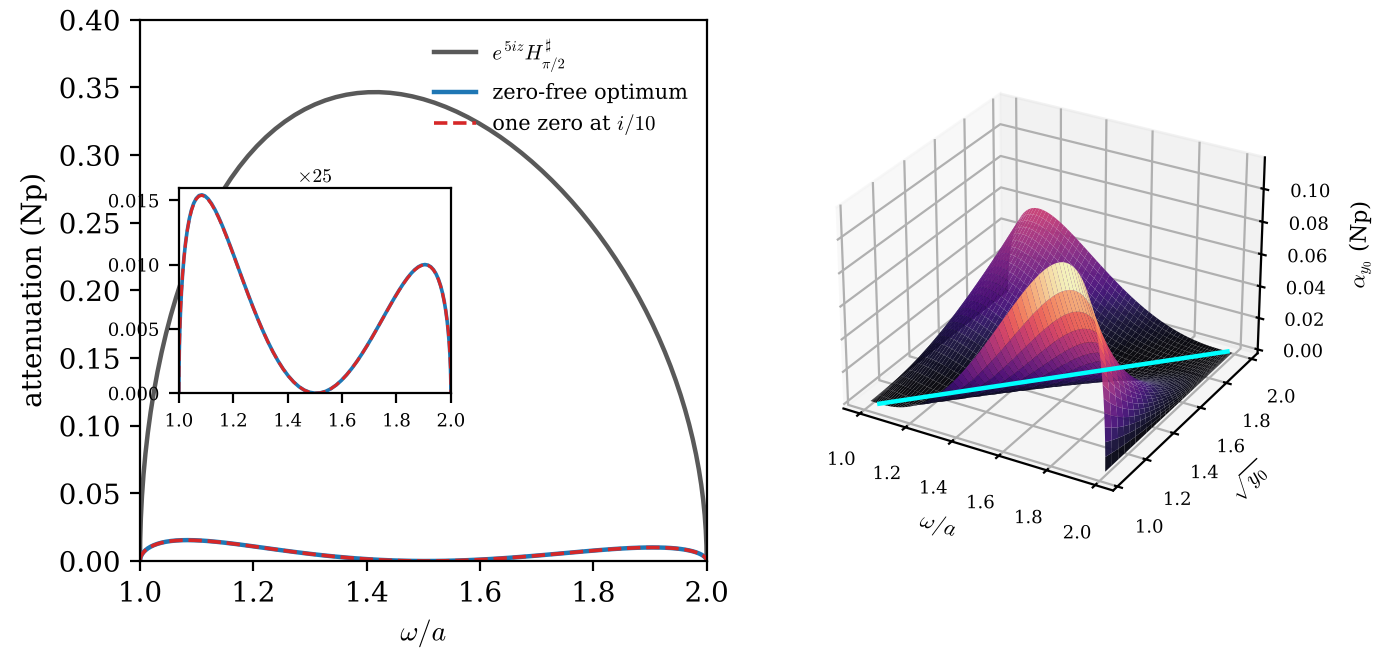
\includegraphics[width=0.8\textwidth]{figures/fig_delay.png}
\caption{The argument $\pi/2+5\omega$ on an octave. Left: the attenuation of
the delayed optimum $e^{5iz}\Hs_{\pi/2}$ (\cref{thm:allzeros}), of the zero-free
optimum of \cref{thm:exactmean}, which touches zero at $x_*=1.5049$, and of
the system with one zero of \cref{prop:onezerodelay}. Right: the zero-free
systems $H_{y_0}$ of \cref{thm:delay}, each lossless at a different
frequency $\sqrt{y_0}$.}
\label{fig:delay}
\end{figure*}

\begin{figure}[t]
\centering
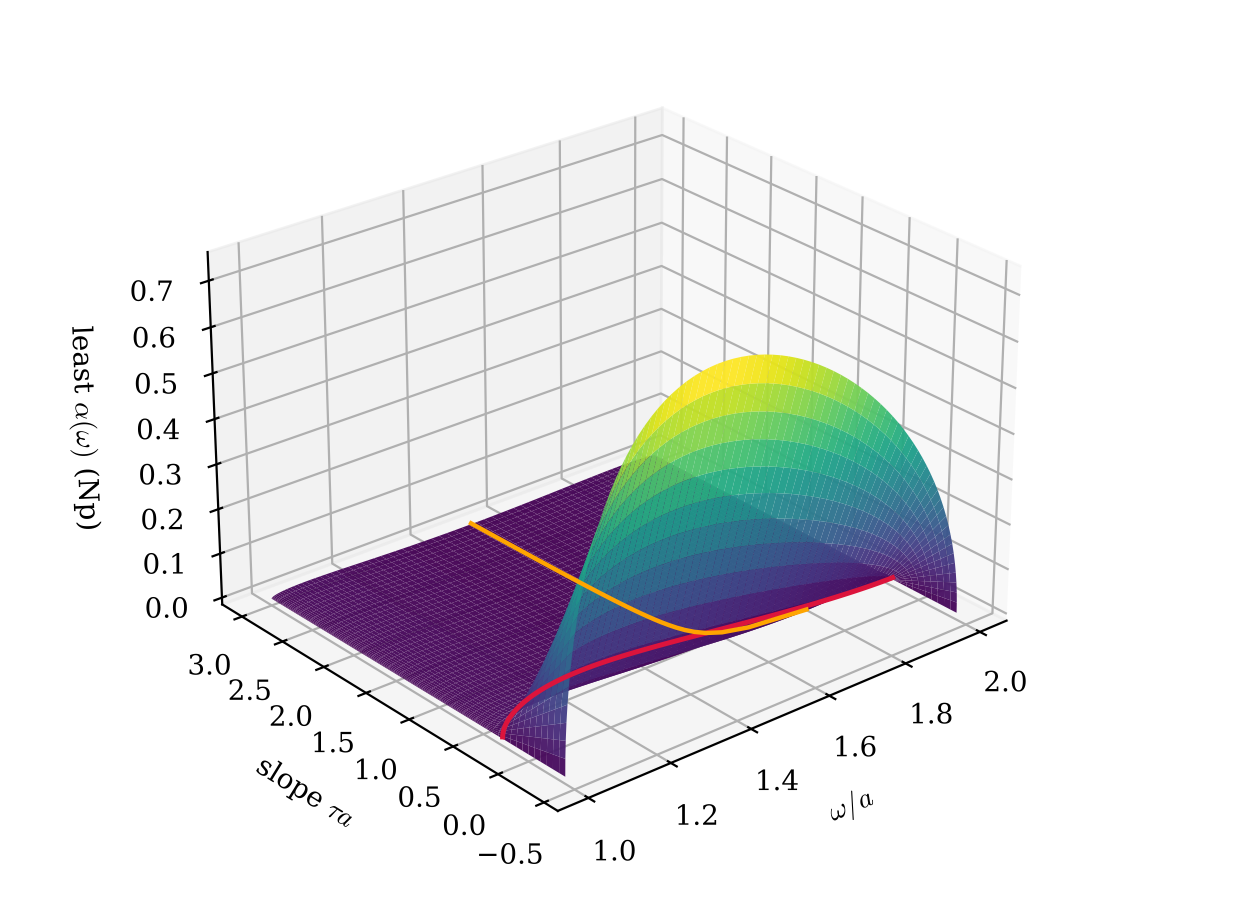
\includegraphics[width=\columnwidth]{figures/fig_exactmean.png}
\caption{The least attenuation of \cref{thm:exactmean} on an octave for the
phase $-1+\tau\omega$, as a function of $\tau$. Up to $\tau_c=0.2852$ it is
pointwise optimal and decreases linearly in $\tau$; beyond it the
resonance above the band moves in from infinity and the profile touches
zero at the contact $x_*$.}
\label{fig:exactmean}
\end{figure}

\subsection{A delay together with zeros}\label{ssec:delayzeros}

\Cref{lem:zeroatom} shows how a zero enters. A zero at $i\varepsilon$ adds
$p_\varepsilon(t)=2\arctan(\varepsilon/t)=2\int_0^\varepsilon j_u(t)\dd u$ to the
phase that the zero-free factor must carry, since $\arg(-B_\varepsilon)=\pi-p_\varepsilon$
on the real axis; and $p_\varepsilon$ costs, in the bound
\eqref{eq:globallower}, what a measure at the negative squared frequencies
$-u^2$ would cost.

\begin{proposition}\label{prop:onezerodelay}
On $[1,2]$, for the argument $\pi/2+5\omega$, there is a passive system with
one zero, at $i/10$, whose mean attenuation is less than
$\mathcal M_{\pi/2}(5)$. So the least zero-free mean is not the least mean
with zeros allowed.
\end{proposition}

\begin{proof}
Let $s=\pi/2$, $\varepsilon=1/10$, $g_0=-s+5t$ and
$g_\varepsilon=g_0+p_\varepsilon$. By \cref{lem:zeroatom},
\begin{gather*}
-\frac{x\,v_{g_\varepsilon}(x)}{r(x)}=q_\varepsilon(x^2),\qquad
q_\varepsilon=sq-P,\\
P(y)=2\int_0^\varepsilon\frac{y\dd u}{(y+u^2)Q_u},\\
\beta_{g_\varepsilon}=5-s\tau_\circ+2\int_0^\varepsilon\frac{\dd u}{Q_u}>0.
\end{gather*}
On $[1,4]$, the integrands of \cref{thm:delay} are at least $1/64$ and $1/512$,
and $\tau_\circ\ge1/2$, as $K(k)\ge\pi/2$, so $q'\ge1/128$ and $-q''\ge1/1024$; and $0\le P'\le
\varepsilon^3/3$, $0\le-P''\le2\varepsilon^3/3$. Hence $q_\varepsilon'>0$ and
$q_\varepsilon''<0$ there. For $\frac94\le y\le4$ the same integral gives
$q-yq'\ge3/32$, and $P\le\varepsilon$, so $q_\varepsilon-yq_\varepsilon'\ge
\frac{3\pi}{64}-\frac1{10}>0$; also $q_\varepsilon(4)\ge\frac\pi8-\varepsilon>0$, since
$q(4)\ge\tau_\circ/2$. The proof of \cref{thm:exactmean}(ii), with $sq$ replaced by
$q_\varepsilon$ and $\tau-s\tau_\circ$ by $\beta_{g_\varepsilon}>-q_\varepsilon(4)$, gives $v>4$ and $C,D>0$ with
$x_*=x(v)\in(\frac32,2)$, and the Herglotz function
$h_\varepsilon=h_{g_\varepsilon}+R(C/z+Dz/(v-z^2))$ with linear coefficient $0$.
The system $H_\varepsilon=-B_\varepsilon e^{ih_\varepsilon}$ is passive, has one zero, at
$i\varepsilon$, and $\arg H_\varepsilon=\pi-p_\varepsilon+g_\varepsilon=\pi/2+5\omega$ on the
band.

For a phase $g$ and this $x_*$, let
$\mathcal L(g)=\int_a^bv_g-\lambda_1x_*v_g(x_*)/r(x_*)-\lambda_2\beta_g$. The
proof of \eqref{eq:globallower} shows that $\int_a^b\alpha\ge\mathcal L(g)$
for every zero-free admissible system with phase $g$, with equality for
$h_\varepsilon$. By \cref{lem:zeroatom},
\[
\mathcal L(j_u)=\frac1{Q_u}\Big(\Gamma_-(-u^2)-\lambda_1\frac{y_*}{y_*+u^2}-\lambda_2\Big),
\]
For $w<0$ put $x(w)=(w+\sqrt{(a^2-w)(b^2-w)}+ab)/(a+b)$, which lies in
$(ab/f,f)$, and $\rho=x(w)-f\in(-\ell^2/f,0)$. Then again
$w=f^2+\ell^2+f(\rho+\ell^2/\rho)$, and $\pi f\rho=-\Gamma_-(w)$. The identity
\eqref{eq:square} is a polynomial identity in $\rho$ and $\varepsilon$, so with
$\Gamma_+(w)$ replaced by $-\Gamma_-(w)$ it reads
\begin{multline*}
(y_*-w)\Big(\Gamma_-(w)-\lambda_1\frac{y_*}{y_*-w}-\lambda_2\Big)\\
=\pi f\Big(f+\frac{\ell^2}\rho\Big)(\rho-x_*+f)^2<0,
\end{multline*}
because $f+\ell^2/\rho<0$. With $w=-u^2$ this gives $\mathcal L(j_u)<0$, so
$\mathcal L(p_\varepsilon)=2\int_0^\varepsilon\mathcal L(j_u)\dd u<0$. The Blaschke
factor has modulus $1$ on $\R$, and
\[
\int_1^2\alpha_{H_\varepsilon}=\mathcal L(g_0)+\mathcal L(p_\varepsilon)
<\mathcal L(g_0)\le\mathcal M_{\pi/2}(5),
\]
the last step by \eqref{eq:globallower} for $g_0$.
\end{proof}

The mean of $H_{1/10}$ is
\[
-s\Lambda+2\int_0^{1/10}\frac{\Gamma_-(-u^2)}{Q_u}\dd u+C\,\Gamma_0+D\,\Gamma_+(v)
=0.0063752
\]
nepers, against $\mathcal M_{\pi/2}(5)=0.0063903$.

\begin{remark}[computed, not proved]\label{rem:onezerofamily}
The construction of \cref{prop:onezerodelay} works for every height
$\varepsilon$ of the zero up to $\varepsilon_0=0.47247$, where the origin
coefficient $C$ vanishes, and the mean then decreases to $0.0051493$ nepers.
With a pair of zeros at $\pm1.3654+1.2608i$ instead, a linear program for
the measure off the band, with the positivity of the attenuation imposed at
$399$ points of the band, gives about $4.3\times10^{-4}$ nepers; without zeros
the same program gives $0.00658$ in place of $0.0063903$, so it is accurate to
a few per cent. These numbers come from computations only. \Cref{prop:sixtap} below proves a mean less than
$7\times10^{-4}$ with six taps.
\end{remark}

\emph{The optimum exists.} The admissible systems are not a convex set, but
a weaker class is. For a measurable $\psi$ on $[a,b]$ let $\mathcal P_\psi$ be
the set of passive systems $H$ with $e^{-i\psi}H\ge0$ almost everywhere on
$[a,b]$, and put
\[
J(H)=\int_a^b-\log\abs{H(\omega)}\dd\omega\in[0,\infty] .
\]
Systems in $\mathcal P_\psi$ may have zeros and need not be regular on the
band. Every system admissible for $\theta$ lies in $\mathcal P_\theta$, and the
systems of \cref{prop:onezerodelay,thm:poisson,thm:expdecay} lie in
$\mathcal P_{\theta+\tau\omega}$.

\begin{theorem}\label{thm:convex}
Let $\psi$ be measurable on $[a,b]$, and suppose that $J(G)<\infty$ for some
$G\in\mathcal P_\psi$.
\begin{enumerate}
\item[(i)] There is exactly one $H_\psi\in\mathcal P_\psi$ with
$J(H_\psi)=\inf_{\mathcal P_\psi}J$.
\item[(ii)] An $H\in\mathcal P_\psi$ with $J(H)<\infty$ is $H_\psi$ if and only if
\[
\int_a^b\frac{\abs{G}}{\abs H}\dd\omega\le b-a\qquad\text{for every }G\in\mathcal P_\psi .
\]
\item[(iii)] Every $G\in\mathcal P_\psi$ satisfies
$\int_a^b\abs{G-H_\psi}^2\dd\omega\le2\big(J(G)-J(H_\psi)\big)$.
\item[(iv)] For $z\in\Cp$ let $P_z(t)=\Im z/(\pi\abs{t-z}^2)$,
$\omega_z=\int_SP_z$ and $M_z=\max_SP_z$, with $S=[-b,-a]\cup[a,b]$. Then
\[
\abs{G(z)-H_\psi(z)}\le2^{1-\omega_z}\Big(\frac{4M_z}{\omega_z}\big(J(G)-J(H_\psi)\big)\Big)^{\omega_z/2}.
\]
\end{enumerate}
\end{theorem}

\begin{proof}
The conditions $\abs H\le1$, $H(-\bar z)=\overline{H(z)}$ and $e^{-i\psi}H\ge0$
almost everywhere are kept by convex combinations, so $\mathcal P_\psi$ is
convex. On $\mathcal P_\psi$, $J(H)=\int_a^b-\log(e^{-i\psi}H)$, and $-\log$ is
convex on $[0,\infty)$, so $J$ is convex.

(i) Let $J_*$ be the infimum and $J(H_k)\to J_*$. The boundary functions are
bounded by $1$ in $L^\infty(\R)$, so a subsequence converges weak-$*$ to some
$\phi$. Since $H_k$ is the Poisson integral of its boundary function
\cite[Ch.~I]{garnett}, $H_k(z)\to H(z)$, the Poisson integral of $\phi$, at
every $z\in\Cp$; so $H$ is analytic, $\abs H\le1$, $H(-\bar z)=\overline{H(z)}$,
and $H=\phi$ almost everywhere on $\R$. On $(a,b)$ the boundary functions
converge weakly in $L^2$, so by Mazur's lemma there are convex combinations
$G_k$ of $H_k,H_{k+1},\dots$ with $G_k\to H$ in $L^2(a,b)$, and almost
everywhere along a subsequence. Each $G_k$ lies in $\mathcal P_\psi$, and
$J(G_k)\le\sup_{j\ge k}J(H_j)\to J_*$ by convexity. The limit of the
nonnegative functions $e^{-i\psi}G_k$ is nonnegative, so $H\in\mathcal P_\psi$,
and Fatou's lemma, with $-\log\ge0$ on $[0,1]$ and lower semicontinuous, gives
$J(H)\le J_*$. If $H$ and $H'$ are both minimisers, then $J_*<\infty$, and
$J(\frac12(H+H'))<J_*$ unless $\abs H=\abs{H'}$ almost everywhere on $(a,b)$,
by strict convexity of $-\log$. Then $H=H'$ almost everywhere on $(a,b)$, since
both have argument $\psi$ where they do not vanish, and $H=H'$ by the
boundary uniqueness theorem \cite[Ch.~II]{garnett}.

(ii) Here $H\ne0$ almost everywhere on $(a,b)$. Put $\rho=\abs G/\abs H$. If the
inequality holds, then $-\log\abs G\ge-\log\abs H-(\rho-1)$, and integrating
gives $J(G)\ge J(H)+(b-a)-\int\rho\ge J(H)$. Conversely, let $H=H_\psi$ and
$0<t\le\frac12$. Then $H_t=(1-t)H+tG\in\mathcal P_\psi$ and
$\abs{H_t}=\abs H(1+t(\rho-1))$, so
\[
0\le\frac{J(H_t)-J(H)}t=\int_a^b\frac{-\log\big(1+t(\rho-1)\big)}t\dd\omega .
\]
The integrand is a difference quotient of a convex function of $t$, so it
decreases as $t\downarrow0$, to $1-\rho$, and it is at most $2\log2$ at
$t=\frac12$. By monotone convergence $\int(1-\rho)\ge0$.

(iii) We may take $J(G)<\infty$. Put $\rho_0=e^{-i\psi}H_\psi$ and
$\rho_1=e^{-i\psi}G$, which lie in $(0,1]$ almost everywhere. Since $-\log$ has
second derivative at least $1$ on $(0,1]$,
\begin{multline*}
-\log\big((1-t)\rho_0+t\rho_1\big)\\
\le-(1-t)\log\rho_0-t\log\rho_1-\tfrac12t(1-t)(\rho_1-\rho_0)^2 ,
\end{multline*}
and $\abs{\rho_1-\rho_0}=\abs{G-H_\psi}$. Integrating, and using
$J((1-t)H_\psi+tG)\ge J(H_\psi)$, gives
$\frac12(1-t)\int\abs{G-H_\psi}^2\le J(G)-J(H_\psi)$; let $t\to0$.

(iv) Let $D=G-H_\psi\ne0$, so $\abs D\le2$. As $\log\abs D$ is subharmonic and
bounded above, it lies below the Poisson integral of its boundary values;
with Jensen's inequality for the probability density $P_z/\omega_z$ on $S$,
\[
\log\abs{D(z)}\le(1-\omega_z)\log2+\frac{\omega_z}2\log\Big(\frac1{\omega_z}\int_SP_z\abs D^2\Big).
\]
By the symmetry, $\int_S\abs D^2=2\int_a^b\abs D^2$, and (iii) gives the bound.
\end{proof}

For a constant phase the minimiser is the system of \cref{thm:allzeros}. The
proof of \cref{prop:compare} uses the continuity of $F$ only to pass from
almost every point of the band to every point; without it, it shows
$\alpha\ge\as_\theta$ almost everywhere for every nonconstant $H\in\mathcal
P_\theta$. Hence $H_\theta=\Hs_\theta$ for $0<\theta<\pi$, and by
\cref{thm:convex}(ii) every $G\in\mathcal P_\theta$ has
$\int_a^b\abs G/\abs{\Hs_\theta}\le b-a$. For $\psi=\theta+\tau\omega$ with $\tau>0$
we have not found $H_\psi$ in closed form, but it is the limit of explicit
passive polynomials, each of them the solution of a finite convex problem.%
\footnote{Parts (iii) and (iv) of \cref{thm:convex}, \cref{lem:toeplitz,lem:tail,lem:chebnorm},
\cref{thm:construction,thm:regularity,thm:sharperate}, \cref{prop:sixtap,prop:commuting}
and \cref{cor:allbands} were found with OpenAI's Codex, starting from
\cref{thm:convex,thm:expdecay}; the proofs were checked step by step and every
number recomputed (\cref{app:verification}).}

Fix $\sigma>0$ and put $w(z)=(z-i\sigma)/(z+i\sigma)$, which maps $\Cp$ onto the
unit disc $\mathbb D$. A function $f$ on $\mathbb D$ with $\abs f\le1$ gives the
passive system $H=f\circ w$, and $H(-\bar z)=\overline{H(z)}$ exactly when the
Taylor coefficients $c_k$ of $f$ are real. For $c=(c_0,\dots,c_N)$ let
$T_N(c)$ be the lower triangular Toeplitz matrix with entries $c_{i-j}$ for
$i\ge j$, $0\le i,j\le N$.

\begin{lemma}\label{lem:toeplitz}
If $\abs f\le1$ on $\mathbb D$, then $\|T_N(c)\|\le1$ and
$\sum_{k\le N}c_k^2\le1$. Conversely, if $c\in\R^{N+1}$ and $\|T_N(c)\|\le1$,
then $p_N(w)=\sum_{k=0}^N(1-\frac k{N+1})c_kw^k$ satisfies $\abs{p_N}\le1$ on
$\mathbb D$.
\end{lemma}

\begin{proof}
Multiplication by $f$ is a contraction of the Hardy space $H^2(\mathbb D)$, and
$T_N(c)$ is its compression to the polynomials of degree at most $N$; its
first column has squared norm $\sum_{k\le N}c_k^2$. For the converse let
$\abs w=1$ and $u=(1,\bar w,\dots,\bar w^N)^{\mathsf T}$. The entry $c_k$ occurs
$N+1-k$ times on the $k$-th subdiagonal, so $u^*T_N(c)u=(N+1)p_N(w)$, and
$\abs{u^*T_Nu}\le\|T_N\|\,\|u\|^2=N+1$. The maximum principle gives the bound
in $\mathbb D$.
\end{proof}

The condition $\|T_N(c)\|\le1$ is the linear matrix inequality
$\left(\begin{smallmatrix}I&T_N\\T_N^{\mathsf T}&I\end{smallmatrix}\right)\succeq0$,
so every feasible $c$ gives a system $p_N\circ w$ that is passive in all of
$\Cp$, not only at sampled frequencies. The phase enters through moments.
Let $\psi$ be $C^1$ on $[a,b]$, and for an interval $I=[u,v]\subset[a,b]$ put
\begin{gather*}
A_{I,k}=\int_u^ve^{-i\psi(x)}w(x)^k\dd x,\\
C_I=2j(v)+\int_u^vj\,\abs{\psi'},\qquad j(x)=\frac{x^2+\sigma^2}{2\sigma}.
\end{gather*}
If $\abs f\le1$, then $\int_Ie^{-i\psi}H=\sum_kc_kA_{I,k}$, since the boundary
values $\sum c_kw^k$ converge in $L^2$.

\begin{lemma}\label{lem:tail}
$\abs{A_{I,k}}\le C_I/k$ for $k\ge1$, so
$(\sum_{k>N}\abs{A_{I,k}}^2)^{1/2}\le\delta_{N,I}=C_I/\sqrt N$, and for
$\abs f\le1$,
\[
\Big|\int_Ie^{-i\psi}H-\sum_{k=0}^Nc_kA_{I,k}\Big|\le\delta_{N,I} .
\]
\end{lemma}

\begin{proof}
On $(0,\infty)$, $w(x)=e^{it}$ with $t=-2\arctan(\sigma/x)$ and $\dd x/\dd t=j(x)$.
With $\beta(t)=j(x)e^{-i\psi(x)}$, integration by parts in
$A_{I,k}=\int\beta e^{ikt}\dd t$ bounds $k\abs{A_{I,k}}$ by
$j(u)+j(v)+\int_u^v(j'+j\abs{\psi'})=C_I$, as $j'>0$. Then
$\sum_{k>N}k^{-2}\le1/N$, and Cauchy--Schwarz with $\sum c_k^2\le1$ bounds the
tail of the series.
\end{proof}

For an affine phase $\theta+\tau\omega$,
$C_I=(v^2+\sigma^2)/\sigma+\abs\tau\big((v^3-u^3)/(6\sigma)+\sigma(v-u)/2\big)$.
Let $\mathcal D_n$ be the partition of $[a,b]$ into $2^n$ equal intervals, and
let $N_n\to\infty$. The \emph{$n$-th problem} has the unknowns
$c\in\R^{N_n+1}$ and $r_I\ge0$ for $I\in\mathcal D_n$; for a coarser dyadic
interval $r_I$ is the sum over the intervals of $\mathcal D_n$ in it. It asks
for
\begin{gather*}
\|T_{N_n}(c)\|\le1,\qquad0\le r_I\le\abs I\quad(I\in\mathcal D_n),\\
\Big|\sum_{k\le N_n}c_kA_{I,k}-r_I\Big|\le\delta_{N_n,I}\quad(I\in\mathcal D_0\cup\dots\cup\mathcal D_n),
\end{gather*}
and minimises $V_n=\sum_{I\in\mathcal D_n}\abs I\,(-\log(r_I/\abs I))$. Its least
value is $v_n$. The constraints are a matrix inequality and second-order
cones, and the objective is convex.

\begin{theorem}\label{thm:construction}
Let $\psi$ be $C^1$ on $[a,b]$ and suppose that $J(G)<\infty$ for some
$G\in\mathcal P_\psi$.
\begin{enumerate}
\item[(i)] Each $n$-th problem has a minimiser, and $0\le v_n\le J(H_\psi)$.
\item[(ii)] $v_n\to J(H_\psi)$.
\item[(iii)] If $(c^{(n)},r^{(n)})$ is feasible with $V_n\le v_n+\varepsilon_n$
and $\varepsilon_n\to0$, then the passive systems
\[
H_n(z)=\sum_{k=0}^{N_n}\Big(1-\frac k{N_n+1}\Big)c^{(n)}_k\Big(\frac{z-i\sigma}{z+i\sigma}\Big)^k
\]
converge to $H_\psi$ locally uniformly in $\Cp$.
\end{enumerate}
\end{theorem}

\begin{proof}
(i) For $H\in\mathcal P_\psi$ with $J(H)<\infty$, its first $N_n+1$
coefficients and $r_I=\int_I\abs H=\int_Ie^{-i\psi}H$ are feasible by
\cref{lem:toeplitz,lem:tail}, and Jensen's inequality on each interval gives
$V_n\le J(H)$. Taking $H=H_\psi$, $v_n\le J(H_\psi)$. The feasible set is compact
and $V_n$ is lower semicontinuous, so a minimiser exists.

(ii), (iii) The $H_n$ are passive by \cref{lem:toeplitz}. By Montel's theorem a
subsequence converges locally uniformly to some $H$ with $\abs H\le1$, with
coefficients $c_k$; then $c^{(n)}_k\to c_k$ for each $k$, and
$\sum_kc_k^2\le1$. For a fixed dyadic interval $I$, $(A_{I,k})_k$ is square
summable, so splitting the sums at a fixed $K$ gives
$\sum_{k\le N_n}c^{(n)}_kA_{I,k}\to\sum_kc_kA_{I,k}=\int_Ie^{-i\psi}H$; as
$\delta_{N_n,I}\to0$, $r^{(n)}_I\to\int_Ie^{-i\psi}H$, which therefore lies in
$[0,\abs I]$. By the dyadic differentiation theorem $e^{-i\psi}H\ge0$ almost
everywhere, and $H\in\mathcal P_\psi$. For a fixed level $q\le n$, convexity of
$-\log$ gives $V_n\ge\Phi_q^{(n)}=\sum_{I\in\mathcal D_q}\abs I(-\log(r^{(n)}_I/\abs I))$,
and in the limit
\[
\liminf_nV_n\ge\Phi_q(H)=\sum_{I\in\mathcal D_q}\abs I\Big(-\log\frac1{\abs I}\int_I\abs H\Big).
\]
By Jensen's inequality $\Phi_q(H)$ increases with $q$ and is at most $J(H)$;
the averages of $\abs H$ converge to $\abs H$ almost everywhere, so Fatou's
lemma gives $\Phi_q(H)\to J(H)$. Hence
$J(H_\psi)\le J(H)\le\liminf V_n\le\liminf(v_n+\varepsilon_n)\le J(H_\psi)$. So
$H=H_\psi$ by \cref{thm:convex}(i), the limit does not depend on the
subsequence, and $v_n\to J(H_\psi)$.
\end{proof}

The finite problems carry the phase only through the moments, so the $H_n$
do not have the phase $\psi$ exactly; it is attained in the limit.
\Cref{thm:construction} gives neither a closed form for $H_\psi$ nor a rate
for $v_n\to J(H_\psi)$. For an analytic phase the optimum has no zeros inside
the band.

\begin{theorem}\label{thm:regularity}
Let $\psi$ be real analytic on $(a,b)$, and suppose that some
$G\in\mathcal P_\psi$ with $J(G)<\infty$ is continuous and nonzero on $(a,b)$.
Then $H_\psi$ extends analytically across $(a,b)$, has no zeros there, and
its attenuation is real analytic on $(a,b)$.
\end{theorem}

\begin{proof}
Near $x_0\in(a,b)$, $F=e^{-i\psi}H_\psi$ is bounded and analytic on the upper
side, and its boundary values are real almost everywhere. Its imaginary part
is a bounded harmonic function, hence the Poisson integral of its boundary
values, which vanish on the interval; so it is continuous up to the
interval with value $0$, and the Schwarz reflection principle continues $F$
across it. On the interval $F\ge0$, and $F\not\equiv0$ because
$J(H_\psi)<\infty$, so a zero at $x_0$ has even order $2k\ge2$ and
$\abs{H_\psi(x)}\le C\abs{x-x_0}^{2k}$ nearby. As $\abs G\ge c>0$ near $x_0$,
$\abs G/\abs{H_\psi}$ is not integrable, against \cref{thm:convex}(ii).
\end{proof}

For every $\psi\in C^1[a,b]$ such a $G$ exists: by \cref{thm:multiband}, with one
band and $n=1$, there is a zero-free passive system with phase $\psi$,
continuous and nonzero on $[a,b]$. So the hypotheses of
\cref{thm:convex,thm:construction} hold for every such phase, and for an
affine phase $H_{\theta+\tau\omega}$ is analytic and has no zeros inside the band,
though it may have zeros in $\Cp$; whether it is continuous at $a$ and $b$ is
not known. The rest of this subsection shows how small its loss is.

There is still a positive floor. For $y>0$ let $P_y(x)=y/(\pi(x^2+y^2))$ and
$\omega_y=\int_a^bP_y$.

\begin{theorem}\label{thm:poisson}
Let $\theta\notin\pi\Z$, $\tau\ge0$ and $H\in\mathcal P_{\theta+\tau\omega}$.
For every $y>0$,
\begin{gather*}
\frac1{b-a}\int_a^b\alpha\ \ge\ \frac{\omega_y}{(b-a)P_y(a)}\,\log\frac1{1-\varepsilon_y}>0,\\
\varepsilon_y=\Big(\frac{\abs{\sin\theta}\,e^{-\tau y}}{2^{1-\omega_y}}\Big)^{1/\omega_y}\in(0,1).
\end{gather*}
\end{theorem}

\begin{proof}
Let $J=H-e^{i\theta+i\tau z}$, analytic in $\Cp$ with $\abs J\le2$. On the
imaginary axis $H(iy)$ is real, so
$\abs{J(iy)}\ge\abs{\sin\theta}e^{-\tau y}>0$. Almost everywhere on the band
$\abs{J(x)}=1-e^{-\alpha(x)}$. As $\log\abs J$ is subharmonic and bounded
above, it lies below the Poisson integral of its boundary values
\cite[Ch.~II]{garnett}, so
\[
\log\big(\abs{\sin\theta}e^{-\tau y}\big)\le\int_a^bP_y\log\big(1-e^{-\alpha}\big)
+(1-\omega_y)\log2 .
\]
Since $u\mapsto\log(1-e^{-u})$ is increasing and concave, Jensen's
inequality for the probability density $P_y/\omega_y$ on $[a,b]$ gives
$\omega_y^{-1}\int_a^bP_y\alpha\ge\log(1/(1-\varepsilon_y))$, and $P_y\le P_y(a)$
on the band.
\end{proof}

The floor is exponentially small in $\tau$, and so is the loss that zeros
make possible. Let $\tau_\circ$ be as in \cref{lem:q}.

\begin{theorem}\label{thm:expdecay}
Let $\theta\in\R$ and $a\tau\ge12$. There is a passive system $H$, regular on the
band, with $\arg H\equiv\theta+\tau\omega$ on $[a,b]$ and
\[
\frac1{b-a}\int_a^b\alpha\le e^{3-a\tau/e}\Big(2+\frac\pi4(b-a)\tau_\circ
+\frac{b(b^2-a^2)}{2e\,a^2}\,\tau\Big).
\]
\end{theorem}

The idea is to turn $\cos\theta+i\sin\theta$ into a function that is close to
$e^{i\theta}$ on the band and is cancelled by the delay $e^{i\tau z}$ in the upper
half-plane: a smoothed sign function of exponential type $\tau$.

\begin{proof}
\emph{The kernel.} Let $m=2\lfloor a\tau/(2e)\rfloor$, so that $m$ is even,
$4\le m\le a\tau/e$ and $m>a\tau/e-2$, and let $\kappa=\tau/m\ge e/a$. Put
\begin{gather*}
I_m=\int_\R\Big(\frac{\sin u}u\Big)^m\dd u,\qquad
T(z)=2\int_0^zK,\\
K(\zeta)=\frac\kappa{I_m}\Big(\frac{\sin\kappa\zeta}{\kappa\zeta}\Big)^m .
\end{gather*}
$K$ is entire, even, nonnegative on $\R$, with $\int_\R K=1$. So $T$ is entire,
odd, real and increasing on $\R$, with $\abs T\le1$ there. Since
$\sin w/w=\int_0^1\cos(tw)\dd t$, $\abs{\sin w/w}\le e^{\abs{\Im w}}$, so
$\abs{K(x+iy)}\le(\kappa/I_m)e^{\tau\abs y}$ and
$\abs{T(x+iy)}\le1+2\kappa e^{\tau\abs y}/(\tau I_m)$.

\emph{The factor $F$.} Let $S=\cos\theta+i\sin\theta\,T$ and $F=e^{i\tau z}S$.
By the last bound $F$ is bounded in $\Cp$; it is continuous up to $\R$ and
$\abs{F(x)}^2=\cos^2\theta+\sin^2\theta\,T(x)^2\le1$ there. So $F$ is the
Poisson integral of its boundary values and $\abs F\le1$ in $\Cp$. As $T$ has
real coefficients and is odd, $F(-\bar z)=\overline{F(z)}$.

\emph{The band.} For $x\ge a$,
\[
0\le1-T(x)=2\int_x^\infty K\le\frac{2(\kappa x)^{1-m}}{(m-1)I_m}\le\varepsilon
=\frac{2(\kappa a)^{1-m}}{(m-1)I_m},
\]
and $0\le T'(x)=2K(x)\le(m-1)\varepsilon/a$. Since $\sin u/u\ge1-u^2/6\ge0$ for
$\abs u\le\sqrt6$ and $(1-v^2)^m\ge1-mv^2$,
\begin{align*}
I_m&\ge\sqrt6\int_{-1}^1(1-v^2)^m\dd v\\
&\ge\sqrt6\int_{\abs v\le m^{-1/2}}(1-mv^2)\dd v
=\frac{4\sqrt6}{3\sqrt m}>\frac3{\sqrt m} .
\end{align*}
With $2\sqrt m\le3(m-1)$, $\kappa a\ge e$ and $m>a\tau/e-2$, this gives
$\varepsilon\le(\kappa a)^{1-m}\le e^{3-a\tau/e}$, and $\varepsilon\le e^{3-12/e}<\frac14$.
On $[a,b]$, $T\in[1-\varepsilon,1]$, so $\abs S\ge1-\varepsilon$ and
$-\log\abs S\le-\log(1-\varepsilon)\le2\varepsilon$. Write
$\arg S=\theta+\delta$ there, with $\delta$ continuous. The derivative of
$\arg(\cos\theta+i\sin\theta\,T)$ in $T$ is
$\sin\theta\cos\theta/(\cos^2\theta+\sin^2\theta\,T^2)$, at most
$\frac12(1-\varepsilon)^{-2}\le\frac89$ in modulus, so $\abs\delta\le\varepsilon$ and
$\abs{\delta'}\le T'\le(m-1)\varepsilon/a$.

\emph{The phase correction.} Let $g=-\delta$ and $G(t)=g(t)/t$ on $[a,b]$. Then
$\abs{G'}\le\abs{\delta'}/a+\abs\delta/a^2\le m\varepsilon/a^2$. By Glauert's
integral (proof of \cref{lem:q}), the function $v_g$ of \cref{prop:profile} is
\[
v_g(x)=\frac{2x\,r(x)}\pi\int_a^b\frac{t\,(G(t)-G(x))}{r(t)\,(x^2-t^2)}\dd t,
\]
and here $\abs{G(t)-G(x)}\le\abs{x^2-t^2}\max\abs{G'}/(2a)$, while
$\int_a^bt\dd t/r(t)=\pi/2$ and $x\,r(x)\le b(b^2-a^2)/2$. So
\[
\abs{v_g}\le\eta=\frac{b(b^2-a^2)\,m\,\varepsilon}{4a^3}
\le\frac{b(b^2-a^2)\,\tau\,\varepsilon}{4e\,a^2} .
\]
Also $\abs{\beta_g}\le\tau_\circ\varepsilon$. Put $c=\max(0,-\beta_g)$ and
$h=h_g+cR/z$. As in the proof of \cref{prop:profile}(iii), $\Im(h_g-\beta_gz)$
is harmonic in $\Cp$, continuous up to $\R$, zero on $\R\setminus S$, equal to
$v_g\ge-\eta$ on the band, and tends to $0$ at infinity, so
$\Im h_g\ge\beta_g\Im z-\eta$. By \cref{lem:R}, $R(0)=-ab$, $R$ is even and
$R(z)=z^2+O(1)$, so $(R+ab)/z-z$ is analytic in $\C\setminus S$, real on
$\R\setminus S$, $O(z^{-1})$ at infinity, and has imaginary part $r(x)/x\ge0$
on the upper side of the band; hence its imaginary part is nonnegative in
$\Cp$, and $\Im(R/z)\ge\Im z+ab\Im(-1/z)\ge\Im z$. So
\[
\Im h\ge(\beta_g+c)\Im z-\eta\ge-\eta\qquad\text{in }\Cp .
\]

\emph{The system.} Let $H=e^{-\eta}F\,e^{ih}$. Then $\abs H\le1$ in $\Cp$, and
$H(-\bar z)=\overline{H(z)}$ because $h$ is odd and real on $\R\setminus S$. It
is continuous up to an open interval around $[a,b]$ and has no zeros there.
On the band $\Re h=g=-\delta$, so $\arg H=\tau\omega+\theta+\delta-\delta=\theta+\tau\omega$,
and
\[
\alpha=\eta-\log\abs S+v_g+c\,\frac rx .
\]
With $\int_a^br/x=\frac\pi4(b-a)^2$ the mean is at most
$2\eta+2\varepsilon+\frac\pi4(b-a)\tau_\circ\varepsilon$, which is the bound.
\end{proof}

For $\theta=\pi/2$ the factor $S=iT$ already has the exact argument $\pi/2$, so
$h=0$, $\eta=0$ and $\alpha=-\log T$. On the octave its mean is
$1.7\times10^{-3}$ nepers at $\tau=12$, $4.9\times10^{-5}$ at $\tau=20$ and
$1.4\times10^{-7}$ at $\tau=30$, against the zero-free floor $0.0060483$ of
\cref{prop:floor}.

A polynomial kernel in $\sin dz$ in place of the sinc power gives a larger
exponent. Approximating the sign by polynomials and entire functions is
classical \cite{eremenkoyuditskii}, as are linear-phase filters with finitely
many taps \cite{parksmcclellan}; we need only the explicit kernel below, whose
passivity is checked directly. Put
\begin{gather*}
d=\frac\pi{a+b},\qquad s_0=\sin da,\qquad \gamma=\operatorname{artanh}s_0,\\
C_{a,b}=\frac\gamma d=\frac{a+b}\pi\log\cot\frac{\pi(b-a)}{4(a+b)} .
\end{gather*}
As $\operatorname{artanh}(\sin t)=\int_0^t\sec u\dd u>t$ for $0<t<\pi/2$,
$C_{a,b}>a$. With the Chebyshev polynomial $T_m$, $T_m(\cos t)=\cos mt$, let
\begin{gather*}
K_m(s)=T_m\Big(\frac{2s^2-1-s_0^2}{1-s_0^2}\Big)^2,\\
\mathcal I_m=\int_0^1K_m,\qquad \Pi_m(s)=\frac1{\mathcal I_m}\int_0^sK_m .
\end{gather*}
$\Pi_m$ is an odd polynomial of degree $4m+1$, increasing on $[-1,1]$ from $-1$
to $1$. For $s_0\le s\le1$ the argument of $T_m$ lies in $[-1,1]$, so
$K_m(s)\le1$ and $0\le1-\Pi_m(s)\le\epsilon_m=(1-s_0)/\mathcal I_m$. On $[a,b]$,
$\sin d\omega\in[s_0,1]$, so $U_m(\omega)=\Pi_m(\sin d\omega)$ satisfies
$1-\epsilon_m\le U_m\le1$ and $\abs{U_m'}\le d/\mathcal I_m$ there.

\begin{lemma}\label{lem:chebnorm}
For $\tau\ge(4m+1)d$ the function
$F_m(z)=e^{i\tau z}(\cos\theta+i\sin\theta\,\Pi_m(\sin dz))$ is passive, and
$\log\mathcal I_m/m\to4\gamma$ as $m\to\infty$.
\end{lemma}

\begin{proof}
Put $q=e^{idz}$ and $N=4m+1$. As $\Pi_m$ is odd with real coefficients,
$q^N(\cos\theta+i\sin\theta\,\Pi_m((q-q^{-1})/(2i)))$ is a polynomial in $q$
with real coefficients. On $\abs q=1$ its modulus is at most $1$, since
$\abs{\Pi_m}\le1$ on $[-1,1]$, so it is at most $1$ for $\abs q\le1$, that is,
in $\Cp$; and $e^{i(\tau-Nd)z}$ is a delay. For $0\le s<s_0$ put
$\chi(s)=\operatorname{arcosh}((1+s_0^2-2s^2)/(1-s_0^2))$, decreasing, with
$\chi(0)=2\gamma$ since $\cosh2\gamma=(1+s_0^2)/(1-s_0^2)$. There
$K_m=\cosh^2(m\chi)$, so $K_m\le e^{4m\gamma}$ on $[0,1]$ and
$\mathcal I_m\le e^{4m\gamma}$; and for $0<h<s_0$,
$\mathcal I_m\ge\int_0^h\frac14e^{2m\chi}\ge\frac h4e^{2m\chi(h)}$. Let
$m\to\infty$ and then $h\to0$.
\end{proof}

\begin{theorem}\label{thm:sharperate}
Let $\theta\in\R$, $m\ge1$, $\tau\ge(4m+1)d$ and $\epsilon_m\le\frac14$. There
is a passive system, regular on the band, with $\arg H\equiv\theta+\tau\omega$ on
$[a,b]$ and
\[
\frac1{b-a}\int_a^b\alpha\le\frac1{\mathcal I_m}\Big(2D_{a,b}+\big(2+\tfrac\pi4(b-a)\tau_\circ\big)(1-s_0)\Big),
\]
where $D_{a,b}=\frac{b(b^2-a^2)}{4a}\big(\frac da+\frac{1-s_0}{a^2}\big)$. For
$\theta=\pi/2$ the system $F_m$ itself has the phase, with mean at most
$2\epsilon_m$.
\end{theorem}

\begin{proof}
Let $S=\cos\theta+i\sin\theta\,U_m$, so that $F_m=e^{i\tau z}S$ is passive by
\cref{lem:chebnorm}. On the band $\abs S\ge1-\epsilon_m$, so
$-\log\abs S\le2\epsilon_m$, and, by the derivative bound in the proof of
\cref{thm:expdecay}, $\arg S=\theta+\delta$ with $\abs\delta\le\epsilon_m$ and
$\abs{\delta'}\le\abs{U_m'}\le d/\mathcal I_m$. The phase correction and the
system are then built as in that proof: with $g=-\delta$ and $G=g/t$,
$\abs{G'}\le\abs{\delta'}/a+\abs\delta/a^2\le(d/a+(1-s_0)/a^2)/\mathcal I_m$, so
Glauert's integral gives $\abs{v_g}\le\eta=D_{a,b}/\mathcal I_m$, and
$\abs{\beta_g}\le\tau_\circ\epsilon_m$. The mean of $e^{-\eta}F_me^{ih}$ is at most
$2\eta+2\epsilon_m+\frac\pi4(b-a)\tau_\circ\epsilon_m$. For $\theta=\pi/2$,
$F_m=ie^{i\tau z}U_m$, $U_m>0$ on the band, and $-\log U_m\le2\epsilon_m$.
\end{proof}

With $m=\lfloor(\tau/d-1)/4\rfloor$, \cref{lem:chebnorm} turns this bound into
$e^{-(C_{a,b}+o(1))\tau}$. On the octave $d=\pi/3$, $s_0=\sqrt3/2$,
$\gamma=\log(2+\sqrt3)$ and
\[
C_{1,2}=\frac3\pi\log(2+\sqrt3)=1.2576021548\ldots,
\]
against $1/e$ from \cref{thm:expdecay}. For the octave, $\Pi_1(s)$ is the
polynomial $P$ below, since $8s^2-7=(2s^2-1-s_0^2)/(1-s_0^2)$; taking $d=1$ in
place of $\pi/3$ lowers the delay $(4m+1)d$ to $5$, at the price of a band
image $[\sin1,1]$ slightly larger than $[s_0,1]$.

\begin{proposition}\label{prop:sixtap}
On $[1,2]$, the passive system
\begin{multline*}
H(z)=\frac1{734}\big(-12-80e^{2iz}-435e^{4iz}\\
+435e^{6iz}+80e^{8iz}+12e^{10iz}\big)
\end{multline*}
has the argument $\pi/2+5\omega$ on the band, no zeros on the band, and
\[
\int_1^2\alpha<\frac7{10000} .
\]
\end{proposition}

\begin{proof}
Let $P(s)=(192s^5-560s^3+735s)/367$. From $\sin3x=3\sin x-4\sin^3x$ and
$\sin5x=16\sin^5x-20\sin^3x+5\sin x$,
$367P(\sin x)=435\sin x+80\sin3x+12\sin5x$, so $H=ie^{5iz}P(\sin z)$. Now
$P(\pm1)=\pm1$ and $P'(s)=\frac{15}{367}(8s^2-7)^2\ge0$, so $\abs P\le1$ on
$[-1,1]$, and $H$ is passive as in \cref{lem:chebnorm}, with $d=1$ and degree
$5$. On $[1,2]$, $\sin x\ge\sin1$, as $\sin$ is concave there and
$\sin2=\sin(\pi-2)>\sin1$, and $\sin1>1-\frac16+\frac1{120}-\frac1{5040}>\frac56$, so
\[
1\ge P(\sin x)>P(\tfrac56)=\frac{59225}{59454}=M,
\]
which gives the argument and the absence of zeros, and $-\log P\le(1-P)/M$.
With $F(t)=t+\frac{176}{1101}t^3+\frac{192}{1835}t^5$ one has
$\frac{\dd}{\dd x}\big(-F(\cos x)\big)=P(\sin x)$, so
$\int_1^2P(\sin x)\dd x=F(\cos1)-F(\cos2)$. The partial sums
$L=\sum_{k=0}^{11}(-1)^k/(2k)!$ and $U=\sum_{k=0}^{12}(-1)^k4^k/(2k)!$ of the
alternating cosine series satisfy $L<\cos1$ and $\cos2<U$, and $F$ is
increasing, so
\[
\int_1^2\alpha\le\frac{1-F(L)+F(U)}M=0.00069587\ldots<\frac7{10000},
\]
the last inequality between rational numbers.
\end{proof}

The mean of this $H$ is $0.00069359$ nepers, against $0.0063752$ for the
one-zero system of \cref{prop:onezerodelay}, $\mathcal M_{\pi/2}(5)=0.0063903$
without zeros, and the zero-free floor $0.0060483$ of \cref{prop:floor}. Its
zeros in $\Cp$ are the points where $\sin z$ is a root of
$192s^4-560s^2+735$, that is, $s^2=(35\pm14i\sqrt5)/24$.

\begin{corollary}\label{cor:rate}
Let $\theta\notin\pi\Z$, and let $E_\theta(\tau)=J(H_{\theta+\tau\omega})/(b-a)$
be the least mean attenuation for the argument $\theta+\tau\omega$, with or
without zeros. Then $E_\theta$ is nonincreasing in $\tau\ge0$, and
\[
-\frac{\pi ab}{b-a}\le\liminf_{\tau\to\infty}\frac{\log E_\theta(\tau)}\tau
\le\limsup_{\tau\to\infty}\frac{\log E_\theta(\tau)}\tau\le-C_{a,b} .
\]
\end{corollary}

\begin{proof}
Multiplication by $e^{i\delta z}$, $\delta\ge0$, maps
$\mathcal P_{\theta+\tau\omega}$ into $\mathcal P_{\theta+(\tau+\delta)\omega}$ and keeps
$\abs H$ on $\R$, which gives the monotonicity; \cref{thm:sharperate} with
$m=\lfloor(\tau/d-1)/4\rfloor$ and \cref{lem:chebnorm} give the upper bound. For the lower bound take
$y=\tau^{-1/2}$ in \cref{thm:poisson}. As $y\to0$,
$\omega_y/y=\frac1\pi\int_a^b\dd x/(x^2+y^2)=\frac{b-a}{\pi ab}+O(y^2)$ and
$\omega_y/P_y(a)\to a(b-a)/b$. With $\log(1/(1-\varepsilon))\ge\varepsilon$,
\begin{align*}
\log E_\theta(\tau)&\ge\log\varepsilon_y+O(1)
=-\frac{\tau y}{\omega_y}+O\Big(\frac1y\Big)\\
&=-\frac{\pi ab}{b-a}\,\tau+O\big(\tau^{1/2}\big).\qedhere
\end{align*}
\end{proof}

So with zeros the least loss for a delay falls off exponentially in the
delay, while without zeros it stays above $(\pi-\vartheta)m_\infty$ or
$\vartheta\Lambda$. On the octave the exponent lies between $-2\pi$ and
$-1.2576$. The optimal system $H_{\theta+\tau\omega}$ is the limit of
\cref{thm:construction}, but its closed form, and the exact exponent, remain
open; the limit in \cref{thm:construction} is taken at fixed $\tau$ and says
nothing about $\tau\to\infty$.

\subsection{Several channels}\label{ssec:channels}

A \emph{generator} on the band is an $n\times n$ matrix function $F$,
analytic in $\Cp$, with $\Im F=(F-F^*)/(2i)\succeq0$ there,
$F(-\bar z)=-F(z)^*$, and continuous up to an open interval $I\supset[a,b]$;
its \emph{phase} and \emph{attenuation} on the band are $\Re F=(F+F^*)/2$ and
$\Im F$ at $x+i0$. For every $u\in\C^n$, $h_u=u^*Fu$ is a Herglotz function
with the symmetry of \eqref{eq:Hh}, continuous up to $I$, so $e^{ih_u}$ is
a zero-free passive system regular on the band, with phase $u^*(\Re F)u$
and attenuation $u^*(\Im F)u$. For a Hermitian matrix $B$, $B_+$ denotes its
positive part.

\begin{theorem}\label{thm:trace}
Let $\Theta$ and $T$ be Hermitian, $B=\tau_\circ\Theta+T$. Every generator
with phase $\Theta+\omega T$ on the band satisfies
\[
\operatorname{tr}\Im F(x)\ge A(x)\operatorname{tr}\Theta+\frac{r(x)}x\operatorname{tr}(-B)_+
\qquad(a\le x\le b).
\]
If $\Theta\succeq0$, equality holds at every point for
$F_{\rm opt}=h_\circ\Theta+zT+(-B)_+R/z$, so that the least mean of
$\operatorname{tr}\Im F$ is
$\Lambda\operatorname{tr}\Theta+\frac\pi4(b-a)\operatorname{tr}(-B)_+$.
\end{theorem}

\begin{proof}
Let $u_1,\dots,u_n$ be an orthonormal basis of eigenvectors of $B$. The
scalar system of $u_j$ has phase $u_j^*\Theta u_j+\omega\,u_j^*Tu_j$, so by
\cref{cor:compare} and \eqref{eq:affinehg} its attenuation is at least
$(u_j^*\Theta u_j)A+(r/x)\max\{0,-u_j^*Bu_j\}$. Summing over $j$ gives the
bound. For $\Theta\succeq0$, $F_{\rm opt}$ has the linear coefficient
$B+(-B)_+=B_+\succeq0$, the origin atom $ab(-B)_+$ and the band density
$\pi^{-1}(A\Theta+(r/x)(-B)_+)\succeq0$ (\cref{lem:atoms}), so
$\Im F_{\rm opt}\succeq0$ in $\Cp$, and its trace attains the bound.
\end{proof}

No commutation of $\Theta$ and $T$ is needed. The trace is the right
objective: the stronger statement, a single generator below all others in
the Loewner order, is false.

\begin{theorem}\label{thm:noloewner}
Let $A_0=\operatorname{diag}(1,-1)$, $T=-\tau_\circ I-A_0$, and consider the
phase $I+\omega T$ on any band. There are generators with this phase, but no
generator $F$ with this phase satisfies $\Im F\preceq\Im G$ on the band for
every generator $G$ with this phase.
\end{theorem}

\begin{proof}
For $C\succeq0$ with $C-A_0\succeq0$, $F_C=h_\circ I+zT+CR/z$ is a generator
with this phase: its linear coefficient is $C-A_0$, its origin atom $abC$ and
its band density $\pi^{-1}(AI+(r/x)C)$. This holds for
\[
C_1=\begin{pmatrix}1&0\\0&0\end{pmatrix},\qquad
C_2=\frac14\begin{pmatrix}5&2\\2&1\end{pmatrix},
\]
since $C_2$ and $C_2-A_0$ have positive diagonals and determinant $1/16$.
The scalar systems of $e_1$ and $e_2$ have phases $1-(\tau_\circ+1)\omega$ and
$1-(\tau_\circ-1)\omega$, so by \cref{thm:affine} the diagonal entries of
$\Im F$ are at least $A+r/x$ and $A$, the diagonal of $\Im F_{C_1}$. If
$\Im F\preceq\Im F_{C_1}$, the difference is positive semidefinite with zero
diagonal, hence zero, and $\Im F=\Im F_{C_1}$. But
$\Im F_{C_2}-\Im F_{C_1}=(r/x)(C_2-C_1)$, and $C_2-C_1$ has the eigenvalues
$3/4$ and $-1/4$.
\end{proof}

When $\Theta$ and $T$ commute the indefinite case reduces to scalars. Let
$\mathcal E(\theta,t)$ be the infimum of the mean of $\Im h$ over scalar
generators $h$ with phase $\theta+\omega t$: by \cref{thm:trace} with $n=1$ for
$\theta\ge0$, and $\mathcal M_{-\theta}(t)$ of \cref{ssec:exactmean} for $\theta<0$.

\begin{proposition}\label{prop:commuting}
If $\Theta T=T\Theta$, with joint eigenvalues $(\theta_j,t_j)$, the infimum of
the mean of $\operatorname{tr}\Im F$ over generators with phase $\Theta+\omega T$
is $\sum_j\mathcal E(\theta_j,t_j)$, and it is attained exactly when each
$\mathcal E(\theta_j,t_j)$ is.
\end{proposition}

\begin{proof}
In a joint orthonormal eigenbasis $u_j$, each $u_j^*Fu_j$ is a scalar
generator with phase $\theta_j+\omega t_j$, and
$\operatorname{tr}\Im F=\sum_ju_j^*(\Im F)u_j$; this gives the lower bound.
Conversely, scalar generators $h_j$ with these phases give the generator
$\sum_jh_ju_ju_j^*$, whose trace is $\sum_j\Im h_j$.
\end{proof}

For noncommuting $\Theta$ and $T$ with $\Theta$ indefinite the least trace is not
known.

\subsection{Several bands}\label{ssec:bands}

Let $0<a_1<b_1<a_2<\dots<a_m<b_m$, choose $c_j\in(b_j,a_{j+1})$ in each gap,
and let $R_m$ be the branch of $\big(\prod_j(z^2-a_j^2)(z^2-b_j^2)\big)^{1/2}$
in the complement of the bands $\pm[a_j,b_j]$ with $R_m\sim z^{2m}$ at
infinity. Put
\[
p(z)=\prod_{j<m}(z^2-c_j^2),\qquad D_m=\frac{R_m}p,\qquad Q_m=\frac{D_m}z .
\]
On the $j$-th positive band $R_m(x+i0)/i$ and $p(x)$ are real with the sign
$(-1)^{m-j}$, so $D_m(x+i0)=i\rho(x)$ with $\rho>0$ on every band.

\begin{lemma}\label{lem:multicomp}
$Q_m$ is an odd Herglotz function with linear coefficient $1$, the atom
$\nu_0=-D_m(0)=\prod_ja_jb_j/\prod_jc_j^2$ at $0$, the atoms
$\nu_j=-\operatorname{Res}_{c_j}Q_m>0$ at $\pm c_j$, the density
$\rho(x)/(\pi x)$ on the bands, and no other measure.
\end{lemma}

\begin{proof}
At $c_j$ the residue is $R_m(c_j)/(2c_j^2\prod_{l\ne j}(c_j^2-c_l^2))$; its
numerator has the sign $(-1)^{m-j}$ and its denominator $(-1)^{m-1-j}$. The
sign of $D_m(0)$ is $(-1)^m(-1)^{m-1}=-1$. Subtracting from $Q_m$ the
corresponding terms of \eqref{eq:foster} leaves an odd function without jumps
across the bands, bounded near their ends and $O(z^{-1})$ at infinity, hence
zero, as in the proof of \cref{lem:atoms}.
\end{proof}

For Hermitian $G_j\in C^1([a_j,b_j])$ define
\[
F_G(z)=\frac{2zD_m(z)}\pi\sum_j\int_{a_j}^{b_j}\frac{G_j(t)\dd t}{\rho(t)\,(z^2-t^2)},
\]
with linear coefficient $B_G$, gap residues $-M_j$ at $c_j$, and band density
$\pi^{-1}V_G$, $V_G(x)=\Im F_G(x+i0)$, all explicit Cauchy integrals.

\begin{theorem}\label{thm:multiband}
The number
\begin{multline*}
c_*=\max\Big\{0,-\lambda_{\min}(B_G),\max_j\frac{-\lambda_{\min}(M_j)}{\nu_j},\\
\sup\lambda_{\max}\Big(-\frac{xV_G(x)}{\rho(x)}\Big)\Big\},
\end{multline*}
the supremum over the open bands, is finite, and for $c\ge c_*$,
$F=F_G+cQ_mI$ is a generator on every band with $\Re F=G_j$ on the $j$-th
band; for $c<c_*$ it is not. For $n=1$, $e^{iF}$ is a zero-free passive
system with phase $G_j$ on each band.
\end{theorem}

\begin{proof}
By the Plemelj formula, as in \cref{prop:profile}(ii), $\Re F_G=G_j$ on the
$j$-th band. There $\rho=r_jL_j$ with
$r_j=\sqrt{(t^2-a_j^2)(b_j^2-t^2)}$ and $L_j>0$ smooth on $[a_j,b_j]$; in
$\sigma=t^2$ the own-band density is $C^1$, and subtracting its value at
$\sigma=x^2$ with Glauert's integral bounds $V_G/\rho$ up to the ends. The
other bands contribute smooth terms. So the supremum is finite. As in
\cref{lem:multicomp}, $F_G$ has the representation \eqref{eq:foster} with
Hermitian coefficients $B_G$, $M_j$ at $\pm c_j$, $\pi^{-1}V_G$ on the bands,
and nothing at $0$. Adding $cQ_mI$ gives $B_G+cI$, $c\nu_0I$, $M_j+c\nu_jI$
and $\pi^{-1}(V_G+c\rho I/x)$, all positive semidefinite exactly when
$c\ge c_*$; the coefficients of a Herglotz representation are unique.
\end{proof}

So every smooth phase on finitely many bands, scalar or matrix, can be
carried by a passive system, at the price of resonances at $0$ and in the
gaps. The theorem minimises only within the family $F_G+cQ_mI$. With zeros
allowed, the weak problem on several bands is solved by the limit of
\cref{thm:construction}.

\begin{corollary}\label{cor:allbands}
Let $B=\bigcup_j[a_j,b_j]$ and let $\psi$ be real and $C^1$ on each band.
\Cref{thm:convex,thm:construction,thm:regularity} hold with $[a,b]$ replaced
by $B$, $b-a$ by $\abs B$ and $\mathcal D_n$ by the dyadic partitions of the
bands, and their hypotheses hold: there is exactly one $H_\psi$ of least
loss in $\mathcal P_\psi$, it is the locally uniform limit of the passive
polynomials $H_n$, and it has no zeros inside the bands if $\psi$ is real
analytic there.
\end{corollary}

\begin{proof}
The proofs use only the measure on the frequency set, so they apply to $B$
unchanged. \Cref{thm:multiband} with $n=1$ gives a zero-free system with phase
$\psi$, continuous and nonzero on $B$, so of finite loss.
\end{proof}

The least loss over zero-free systems on several bands, the behaviour of
$H_\psi$ at the ends of the bands, and the matrix problem with zeros are not
known.

\section{Waves in passive media}\label{sec:waves}

\subsection{A slab of a passive medium}

Consider a plane wave crossing a slab of thickness $L$ of a linear,
homogeneous, isotropic and temporally dispersive medium with relative
permittivity $\epsilon(\omega)$ and permeability $\mu_r(\omega)$. We
consider the propagation factor of a single pass and ignore reflections at
the faces, which is exact for an impedance-matched slab and otherwise
describes the field inside the medium. In our convention the factor is
\[
H(\omega)=\exp\Big(\frac{i\omega n(\omega)L}c\Big),\qquad
n=\sqrt{\epsilon\mu_r}=n_r+in_i .
\]
Passivity of the medium means that $z\epsilon(z)$ and $z\mu_r(z)$ are
Herglotz functions and that $\epsilon$ and $\mu_r$ tend to $1$ as
$z\to i\infty$ \cite{nussenzveig,gustafsson,bernland}. Reality of the fields
makes $\epsilon$ and $\mu_r$ real on $i\R_+$, so that $z\epsilon(z)$ and
$z\mu_r(z)$ lie on the closed positive imaginary axis there.\footnote{Analyticity in $\Cp$ is
causality of the constitutive relations; $\Im(\omega\epsilon(\omega))\ge0$ for
real $\omega$ is the absence of gain; the limit expresses that every medium is
transparent at very high frequency. The Herglotz property in $\Cp$ follows from
these boundary properties by the Poisson representation of the harmonic
function $\Im(z\epsilon(z))$.}

\begin{lemma}\label{lem:index}
$h(z)=zn(z)L/c$ is a Herglotz function with $h(iy)\in i\R$ and
$h(-\bar z)=-\overline{h(z)}$, and its linear coefficient in
\eqref{eq:foster} is $\beta=L/c$. Hence $H=e^{ih}$ is a zero-free passive
system with $\sigma=1$, phase $\varphi=\omega n_rL/c$ and attenuation
$\alpha=\omega n_iL/c$.
\end{lemma}

\begin{proof}
Put $f(z)=z\epsilon(z)$ and $g(z)=z\mu_r(z)$, so that $zn(z)=\sqrt{f(z)g(z)}$.
For $z\in\Cp$, $\arg f$ and $\arg g$ lie in $[0,\pi]$; we take the square
root with argument $\frac12(\arg f+\arg g)\in[0,\pi]$, which is analytic and
is the branch with $n\to1$. So $zn(z)$ maps $\Cp$ to the closed upper
half-plane. On $i\R_+$, $f$ and $g$ lie on $i\R_+$, so their product is
negative and $zn$ lies on $i\R_+$. The symmetry follows from that of $f$ and
$g$, and $\beta=\lim h(iy)/(iy)=L/c$ because $n(iy)\to1$.
\end{proof}

The coefficient $\beta=L/c$ is the vacuum delay: no signal crosses the slab
faster than light. It drops out of the bound, as every delay does.

\begin{theorem}\label{thm:slab}
Let the medium be passive, with $n$ continuous and nonzero on a
neighbourhood of $[a,b]$ in $\overline{\Cp}$, and suppose that on the band
\begin{equation}\label{eq:anomalous}
n_r(\omega)=n_0+\frac C\omega,\qquad a\le\omega\le b,
\end{equation}
with constants $n_0\in\R$ and $C\ge0$. Then
\begin{equation}\label{eq:slab}
\frac1{b-a}\int_a^b\omega\,n_i(\omega)\dd\omega\ \ge\ C\,\Lambda ,
\end{equation}
with equality if and only if the Herglotz measure of $zn(z)$ is carried by
$S$.
\end{theorem}

\begin{proof}
By \cref{lem:index}, $H$ is zero-free, passive and regular on the band, with
phase $\varphi=\omega n_rL/c=CL/c+(n_0L/c)\,\omega$. \Cref{thm:main} with
$\theta=CL/c$ and $\tau=n_0L/c$ gives
$\frac1{b-a}\int\omega n_iL/c\ge(CL/c)\Lambda$, and $L/c$ cancels.
\end{proof}

The thickness of the slab has dropped out: \eqref{eq:slab} is a property of
the material. The condition \eqref{eq:anomalous} says that the phase index
exceeds the group index $n_g=\dd(\omega n_r)/\dd\omega=n_0$ by $C/\omega$, or
equivalently that $\dd n_r/\dd\omega=-C/\omega^2<0$. So
\cref{thm:slab} is a quantitative form of the old observation that
anomalous dispersion requires absorption \cite{kronig,kramers,nussenzveig}:
an index falling like $C/\omega$ across a band requires the frequency-weighted
extinction $\omega n_i$ to be at least $C\Lambda$ on average. In terms of the
intensity absorption coefficient $a_{\rm abs}=2\omega n_i/c$ the bound reads
$\overline{a_{\rm abs}}\ge2C\Lambda/c$.

\begin{figure}[t]
\centering
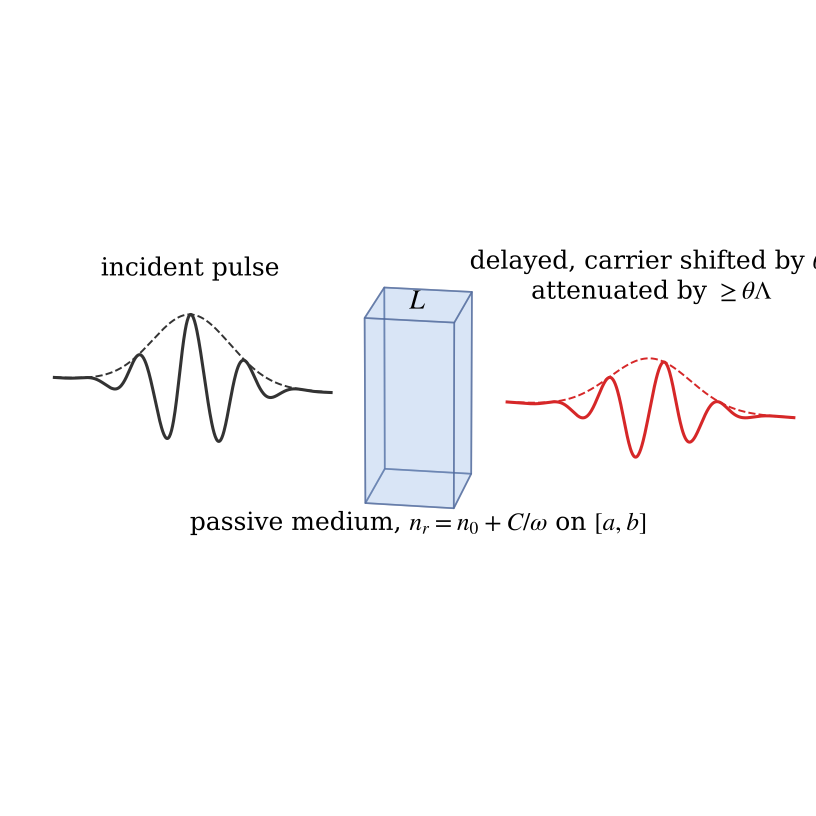
\includegraphics[width=\columnwidth]{figures/fig_slab.png}
\caption{Schematic of \cref{thm:slab}. A pulse crosses a slab of a passive
medium whose index falls like $n_0+C/\omega$ on the band. The envelope is
delayed by $n_0L/c$, the carrier is shifted under it by $\theta=CL/c$, and the
pulse leaves attenuated (the factor is exaggerated). By \cref{thm:slab}
the mean of $\omega n_i$ over the band is at least $C\Lambda$, whatever the
thickness $L$.}
\label{fig:slab}
\end{figure}

\subsection{Approximate constant phase}

The sum rule is linear in the phase, so the bound is stable under
perturbations. Put $P=\int_a^b\abs{p(\omega)}\dd\omega$.

\begin{corollary}\label{cor:stable}
Let $H$ be zero-free, passive and regular on the band, with
$\abs{\varphi(\omega)-\theta-\tau\omega}\le\varepsilon$ on $[a,b]$. Then
\[
\frac1{b-a}\int_a^b\alpha\dd\omega\ \ge\ \theta\Lambda-\frac{P}{2(b-a)}\,\varepsilon .
\]
In particular a zero-free system that is lossless on the band cannot
approximate a constant phase lag $\theta>0$ to within
$\varepsilon<\theta J/P$.
\end{corollary}

\begin{proof}
By \cref{thm:sumrule} and \cref{lem:moments}(i),
$\int_a^b\alpha\ge\frac12\int_a^b\varphi p=\frac12\theta J
+\frac12\int_a^b(\varphi-\theta-\tau\omega)p$, and the last term is at least
$-\frac12\varepsilon P$. If $\alpha=0$ on the band, then
$0\ge\frac12(\theta J-\varepsilon P)$.
\end{proof}

For an octave $J/P=0.2584$, so a lossless zero-free system cannot hold its
phase within $0.258\,\theta$ of any $\theta+\tau\omega$ with $\theta>0$ across
the octave; for the decade $[1,10]$ the ratio is $0.617$. The ratio $J/P$
does not depend on the scale of the band.

\begin{remark}[Broadband phase shifters]\label{rem:darlington}
Broadband ``$90^\circ$ phase shifters'' are pairs of lossless all-pass
networks whose phases differ by approximately $\pi/2$ across a band
\cite{darlington}. Each phase is increasing (\cref{prop:foster}); only their
difference is nearly constant. This is consistent with \cref{cor:stable}:
what the theorem forbids is a lossless network whose own phase is nearly
constant on the band, and a pair of networks never needs one. A device that
shifts a single signal by $\theta$ without a reference channel must lose
transmitted power.
\end{remark}

\subsection{What the bound means for energy}\label{sec:energy}

On the band the power transmission is $T(\omega)=\abs{H(\omega)}^2
=e^{-2\alpha(\omega)}$.

\begin{proposition}\label{prop:energy}
Let $H$ be as in \cref{thm:main} with $\theta>0$.
\begin{enumerate}
\item[(i)] There is $\omega_1\in[a,b]$ with $T(\omega_1)\le e^{-2\theta\Lambda}$,
and for every $\varepsilon>0$ there is a signal with spectrum in
$[-b,-a]\cup[a,b]$ that loses at least the fraction
$1-e^{-2\theta\Lambda}-\varepsilon$ of its energy.
\item[(ii)] The geometric mean of $T$ over the band is at most
$e^{-2\theta\Lambda}$.
\item[(iii)] In a quantised description, a single quantum of frequency
$\omega_1$ fails to be transmitted with probability at least
$1-e^{-2\theta\Lambda}$, and the mean energy it removes from the transmitted
channel is at least $(1-e^{-2\theta\Lambda})\hbar\omega_1$.
\item[(iv)] For a narrow band of relative width $\Delta f/f$ and
$\theta$ in degrees,
$1-e^{-2\theta\Lambda}=\frac{\pi^2}{720}\,\theta\,\frac{\Delta f}f\,
\big(1+O(\theta\Delta f/f)+O((\Delta f/f)^2)\big)$.
\end{enumerate}
\end{proposition}

\begin{proof}
(i) The mean of the continuous function $\alpha$ is at least $\theta\Lambda$,
so $\alpha(\omega_1)\ge\theta\Lambda$ at some $\omega_1$. A signal whose
spectrum is concentrated near $\pm\omega_1$ transmits a fraction of its
energy arbitrarily close to $T(\omega_1)$ by Parseval's identity and the
continuity of $T$. (ii) is \cref{cor:worst}. (iii) A linear lossy element
acts on a single quantum as a beam splitter coupling the transmitted mode
to the other modes of the device; the quantum is transmitted with
probability $T(\omega_1)$. (iv) By \eqref{eq:narrow}, $\Lambda=\frac\pi8\frac{\Delta f}{f}
(1+O((\Delta f/f)^2))$, and $\theta$ degrees are $\pi\theta/180$ radians, so
$2\theta\Lambda=\frac{\pi^2}{720}\theta\frac{\Delta f}f(1+\cdots)$; finally
$1-e^{-x}=x(1+O(x))$.
\end{proof}

The bound is on transmission. The power that is not transmitted may be
absorbed, reflected or routed to other ports, and \cref{prop:energy} does not
say which: a scalar transfer function sees only the output channel. For the
impedance-matched slab of \cref{thm:slab}, which reflects nothing and has no
other port, all of it is absorbed. The energy that is lost is not the
``energy of the phase shift''. A phase
factor is energy neutral (\cref{prop:static}). The loss is the price that
causality and passivity attach to producing that factor on a band.

\subsection{The 5\,MHz example done correctly}

Take the example of \cite{tb23}: a $1^\circ$ phase shift of a wave at
$5$\,MHz, and give it a band, $4.5$ to $5.5$\,MHz, so $\Delta f/f=0.2$. Then
$\kappa=0.1$ and
\begin{gather*}
\Lambda=0.078836,\\
\theta\Lambda=\frac\pi{180}\Lambda=1.3760\times10^{-3}\,\text{Np}
=0.011951\,\text{dB}.
\end{gather*}
A passive device that shifts the carrier--envelope phase by $1^\circ$
across this band therefore fails to transmit at least $0.275\%$ of the power
at its worst frequency, $1-e^{-2\theta\Lambda}=2.748\times10^{-3}$, against
$2.742\times10^{-3}$ from \cref{prop:energy}(iv). A quantum of
$hf=3.313\times10^{-27}$\,J at that frequency removes from the output on average at least
$9.10\times10^{-30}$\,J. This happens to be close to the value
$hf/360=9.20\times10^{-30}$\,J that a phase slipping by $1^\circ$ per period
would remove (\cref{prop:slip}), but the agreement is accidental: the ratio
of the two numbers is $0.989$, close to
$\frac{\pi^2}2\frac{\Delta f}f=0.987$ by \cref{prop:energy}(iv), and it
tends to zero with the bandwidth. For a single sinusoid,
$\Delta f=0$ and a delay of $555.6$\,ps does the job without loss.

\section{Discussion and open problems}\label{sec:discussion}

\subsection{What has been shown}

A passive system can delay a band of frequencies for free, but it cannot
shift the phase of the whole band by a constant without absorbing. The
least mean absorption is $\theta\Lambda$, with $\Lambda=(K(\kappa)-E(\kappa))/\kappa$
an explicit function of the band ratio, and the bound is attained. The proof
is a single sum rule, \eqref{eq:sumrule}, built from the test function $W$,
and every other statement of the paper is a consequence of it or of the
explicit extremal system: the lead bound, the worst-frequency and
geometric-mean bounds, the bound for anomalous dispersion in a medium, and
the stability under perturbations of the phase.

The ingredients are classical: the Herglotz representation, Kramers--Kronig
relations, a Cauchy integral, and an elliptic integral reduced by Landen's
transformation. What is new, as far as we can tell, is the inequality and
its sharpness, and the identification of the price of a constant phase with
a single number $\Lambda$.

\subsection{Open problems}

\begin{enumerate}
\item[(1)] \emph{Systems with zeros.} Determine the infimum of
\cref{prob:zeros}. Even its positivity is open. A first step would be the
best single zero, at an arbitrary point of $\Cp$ rather than on the
imaginary axis, and the best pair of zeros $\zeta,-\bar\zeta$.
\item[(2)] \emph{The plain mean for a lead.} \Cref{thm:lead} is sharp for the
weighted mean. Is the system $H_\star(-ab/z)$ of \cref{rem:leadmean}
optimal for the plain mean, with value $\abs\theta(E-\kappa'^2K)/\kappa$?
\item[(3)] \emph{The worst frequency.} \Cref{cor:worst} bounds $\max\alpha$ by
the mean. The sharp bound on $\max\alpha$ is an extremal problem of
Chebyshev type: minimise $\sup_{[a,b]}\Im h$ among Herglotz functions with
$\Re h=\theta$ on the band. The extremal $H_\star$ has
$\max\alpha_\star/\theta\Lambda=1.273$ for an octave, so the sharp constant
lies between $\Lambda$ and $1.273\Lambda$ there.
\item[(4)] \emph{Several bands.} For a phase that is constant on each of
several disjoint bands, the test function is built from a hyperelliptic
square root, and the constant becomes a period of a hyperelliptic
differential. We expect the sum rule to carry over with the same proof.
\item[(5)] \emph{Reflection and matching.} For reflection coefficients,
the Fano bound \cite{fano} and the present bound constrain different parts
of the same function. A joint bound on the modulus and the argument of a
reflection coefficient on a band would combine the two.
\item[(6)] \emph{Formalisation.} The finite arithmetic of the paper is
checked in Lean (\cref{app:verification}). The analytic part, the sum rule
and the evaluation of $\Lambda$, would require a formalisation of boundary
values of Cauchy integrals, of the M.~Riesz theorem and of the complete
elliptic integrals with Landen's transformation. We have not done this, and
the analytic theorems of the paper are not machine-checked.
\end{enumerate}

\appendix
\section{Complete elliptic integrals}\label{app:elliptic}

This appendix derives every property of $K$ and $E$ used in the paper. The
modulus is $k\in[0,1)$ and the complementary modulus is $k'=\sqrt{1-k^2}$;
we write $K'=K(k')$ and $E'=E(k')$.

\subsection{Power series}

For $\abs u<1$, $(1-u)^{-1/2}=\sum_{n\ge0}c_nu^n$ and
$(1-u)^{1/2}=\sum_{n\ge0}c_nu^n/(1-2n)$, with $c_n=\binom{2n}n4^{-n}$; the
first is the binomial series, $\binom{-1/2}n(-1)^n=c_n$, and the second follows
by integrating the first term by term. The Wallis integral
$\frac2\pi\int_0^{\pi/2}\sin^{2n}\phi\dd\phi=c_n$ follows by induction from
the reduction formula
$\int_0^{\pi/2}\sin^{2n}=\frac{2n-1}{2n}\int_0^{\pi/2}\sin^{2n-2}$ and the
recurrence $c_n=\frac{2n-1}{2n}c_{n-1}$. With $u=k^2\sin^2\phi$ and uniform
convergence for $k<1$,
\begin{equation}\label{eq:KEseries}
K(k)=\frac\pi2\sum_{n\ge0}c_n^2k^{2n},\qquad
E(k)=\frac\pi2\sum_{n\ge0}\frac{c_n^2}{1-2n}k^{2n}.
\end{equation}
Subtracting, $K-E=\frac\pi2\sum_{n\ge1}c_n^2\frac{2n}{2n-1}k^{2n}$, which is
the series of \cref{prop:Lambda}(i).\footnote{The coefficients
$d_n=c_n^2\,2n/(2n-1)$ are $\frac12,\frac3{16},\frac{15}{128},\frac{175}{2048},
\dots$; the ratio $d_{n+1}/d_n=(2n+1)(2n-1)/((2n+2)2n)$ follows from
$c_{n+1}/c_n=(2n+1)/(2n+2)$.}

\subsection{Derivatives}

Differentiating under the integral sign,
\begin{equation}\label{eq:derivs}
\frac{\dd E}{\dd k}=\frac{E-K}k,\qquad
\frac{\dd K}{\dd k}=\frac{E-k'^2K}{k\,k'^2}.
\end{equation}
The first is immediate: $\frac{\dd}{\dd k}\sqrt{1-k^2\sin^2\phi}
=-k\sin^2\phi/\sqrt{\cdot}$, and $-k^2\sin^2\phi=(1-k^2\sin^2\phi)-1$. For the
second, the derivative is $\int_0^{\pi/2}k\sin^2\phi\,(1-k^2\sin^2\phi)^{-3/2}
\dd\phi$, and the identity
\begin{multline*}
\frac{\dd}{\dd\phi}\frac{\sin\phi\cos\phi}{\sqrt{1-k^2\sin^2\phi}}\\
=\frac1{k^2}\Big(\sqrt{1-k^2\sin^2\phi}-\frac{k'^2}{(1-k^2\sin^2\phi)^{3/2}}\Big),
\end{multline*}
integrated over $[0,\pi/2]$, gives $\int(1-k^2\sin^2)^{-3/2}=E/k'^2$; then
$k^2\sin^2\phi(1-k^2\sin^2\phi)^{-3/2}=(1-k^2\sin^2)^{-3/2}-(1-k^2\sin^2)^{-1/2}$
yields \eqref{eq:derivs}.\footnote{To check the displayed identity, put
$s=\sin\phi$, $c=\cos\phi$, $\Delta=1-k^2s^2$. The derivative of $sc\,\Delta^{-1/2}$
is $(c^2-s^2)\Delta^{-1/2}+k^2s^2c^2\Delta^{-3/2}=\Delta^{-3/2}\big((c^2-s^2)\Delta
+k^2s^2c^2\big)$, and with $c^2=1-s^2$ the bracket is
$1-2s^2+k^2s^4=\frac1{k^2}\big(\Delta^2-k'^2\big)$.}

\subsection{Legendre's relation}

\begin{lemma}\label{lem:legendre}
$E(k)K'+E'K(k)-K(k)K'=\pi/2$ for $0<k<1$.
\end{lemma}

\begin{proof}
Let $L(k)$ be the left side. Since $\dd k'/\dd k=-k/k'$, \eqref{eq:derivs}
applied at $k'$ gives
\[
\frac{\dd E'}{\dd k}=\frac{k(K'-E')}{k'^2},\qquad
\frac{\dd K'}{\dd k}=-\frac{E'-k^2K'}{kk'^2}.
\]
Multiply $\dd L/\dd k$ by $kk'^2$ and insert the four derivatives:
\begin{multline*}
kk'^2L'=k'^2(E-K)K'-E(E'-k^2K')+k^2K(K'-E')\\
+E'(E-k'^2K)-K'(E-k'^2K)+K(E'-k^2K').
\end{multline*}
Expanding, the terms in $KK'$ and in $EE'$ cancel in pairs, and what
remains is
\[
kk'^2L'=(k^2+k'^2-1)\,(EK'-KE')=0 .
\]
So $L$ is constant. As $k\to0$, $K,E\to\pi/2$ and $E'\to1$, while
$K-E=O(k^2)$ by \eqref{eq:KEseries} and $K'=O(\log(1/k))$ by
\eqref{eq:Klog} below; hence $L=E'K+(E-K)K'\to\pi/2$.
\end{proof}

\subsection{The arithmetic--geometric mean and Landen's transformation}

For $p,q>0$ let
\[
I(p,q)=\int_0^{\pi/2}\frac{\dd\phi}{\sqrt{p^2\cos^2\phi+q^2\sin^2\phi}},
\]
so that $K(k)=I(1,k')$.

\begin{lemma}[Gauss]\label{lem:gauss}
$I(p,q)=I\big(\frac{p+q}2,\sqrt{pq}\big)$. Consequently
$I(p,q)=\pi/(2M(p,q))$, with $M$ the arithmetic--geometric mean of $p$
and $q$.
\end{lemma}

\begin{proof}
With $x=q\tan\phi$, $I(p,q)=\frac12\int_\R\big((p^2+x^2)(q^2+x^2)\big)^{-1/2}\dd x$.
Substitute $x=\frac12(t-pq/t)$, $t>0$, which maps $(0,\infty)$ increasingly
onto $\R$, with $\dd x=\frac12(1+pq/t^2)\dd t$. Then
$4x^2+(p+q)^2=(t^2+p^2)(t^2+q^2)/t^2$ and $x^2+pq=\frac14(t+pq/t)^2$, so
\[
\big((p_1^2+x^2)(q_1^2+x^2)\big)^{-1/2}\dd x
=\frac{2\,\dd t}{\sqrt{(t^2+p^2)(t^2+q^2)}},
\]
with $p_1=\frac{p+q}2$, $q_1=\sqrt{pq}$. Integrating over $t\in(0,\infty)$
and using that the integrand is even in $t$,
\begin{align*}
2I(p_1,q_1)&=2\int_0^\infty\frac{\dd t}{\sqrt{(t^2+p^2)(t^2+q^2)}}\\
&=\int_\R\frac{\dd t}{\sqrt{(t^2+p^2)(t^2+q^2)}}=2I(p,q).
\end{align*}
The
iterates converge to $M(p,q)$, and $I(M,M)=\pi/(2M)$.
\end{proof}

\begin{proposition}[Landen]\label{prop:landen}
Let $0<k'<1$ and $\kappa=(1-k')/(1+k')$. Then
\[
K(k)=(1+\kappa)K(\kappa),\qquad E(k)=(1+k')E(\kappa)-k'K(k).
\]
\end{proposition}

\begin{proof}
By \cref{lem:gauss}, $K(k)=I(1,k')=I\big(\frac{1+k'}2,\sqrt{k'}\big)
=\frac2{1+k'}I\big(1,\frac{2\sqrt{k'}}{1+k'}\big)$, and
$\frac{2\sqrt{k'}}{1+k'}=\sqrt{1-\kappa^2}=\kappa'$, so
$K(k)=\frac2{1+k'}K(\kappa)=(1+\kappa)K(\kappa)$. For $E$, regard $k$ as a
function of $\kappa$, $k=2\sqrt\kappa/(1+\kappa)$, $k'=(1-\kappa)/(1+\kappa)$,
and differentiate the relation for $K$ with \eqref{eq:derivs}. Since
\begin{gather*}
\frac{\dd k}{\dd\kappa}=\frac{1-\kappa}{\sqrt\kappa(1+\kappa)^2},\qquad
kk'^2=\frac{2\sqrt\kappa(1-\kappa)^2}{(1+\kappa)^3},\\
\text{so}\qquad
\frac{\dd k/\dd\kappa}{kk'^2}=\frac{1+\kappa}{2\kappa(1-\kappa)},
\end{gather*}
the derivative of $K(k)$ is $\big(E(k)-k'^2K(k)\big)\frac{1+\kappa}{2\kappa(1-\kappa)}$,
and that of $(1+\kappa)K(\kappa)$ is
$K(\kappa)+\big(E(\kappa)-(1-\kappa^2)K(\kappa)\big)/(\kappa(1-\kappa))$.
Equating, multiplying by $2\kappa(1-\kappa)/(1+\kappa)$ and using
$k'^2(1+\kappa)=(1-\kappa)^2/(1+\kappa)$,
\begin{align*}
E(k)&=\frac{2E(\kappa)}{1+\kappa}+\frac{K(\kappa)}{1+\kappa}\Big((1-\kappa)^2
+2\kappa(1-\kappa)\\
&\qquad-2(1-\kappa)(1+\kappa)\Big)\\
&=\frac{2E(\kappa)}{1+\kappa}-(1-\kappa)K(\kappa).
\end{align*}
Since $2/(1+\kappa)=1+k'$ and $(1-\kappa)K(\kappa)=k'K(k)$, this is the
claim.
\end{proof}

\subsection{Behaviour at the ends}

As $k\to0$, \eqref{eq:KEseries} gives $K,E=\frac\pi2+O(k^2)$. As $k\to1$,
$E(k)\to1$ and
\begin{equation}\label{eq:Klog}
K(k)=\log\frac4{k'}+O\big(k'^2\log k'\big).
\end{equation}
The limit of $E$ is dominated convergence. For $K$, the substitution
$x=k'\tan\phi$ of \cref{lem:gauss} gives
$K(k)=\int_0^\infty\big((1+x^2)(k'^2+x^2)\big)^{-1/2}\dd x$. Split at $x=1$:
\[
\int_0^1\frac{\dd x}{\sqrt{k'^2+x^2}}=\operatorname{arsinh}\frac1{k'}
=\log\frac2{k'}+o(1),
\]
and, by dominated convergence,
\begin{gather*}
\int_0^1\frac{(1+x^2)^{-1/2}-1}{\sqrt{k'^2+x^2}}\dd x\to\log\frac2{1+\sqrt2},\\
\int_1^\infty\frac{\dd x}{\sqrt{(1+x^2)(k'^2+x^2)}}\to\log(1+\sqrt2),
\end{gather*}
the first limit being
$\int_0^1\big(\frac1{x\sqrt{1+x^2}}-\frac1x\big)\dd x=\log\frac2{1+\sqrt2}$,
both from the primitive $-\operatorname{arsinh}(1/x)$ of
$1/(x\sqrt{1+x^2})$. The three limits add up to $\log(4/k')$.
The error term is \cite[19.12.1]{dlmf}.

\section{The elementary integrals}\label{app:integrals}

\subsection{Moments of the arcsine weight}

For $A<B$ put $m=\frac{A+B}2$, $d=\frac{B-A}2$ and
$\sigma=m-d\cos\phi$, $0\le\phi\le\pi$. Then
$(\sigma-A)(B-\sigma)=d^2\sin^2\phi$ and $\dd\sigma=d\sin\phi\dd\phi$, so
$\dd\sigma/\sqrt{(\sigma-A)(B-\sigma)}=\dd\phi$, and
\begin{align*}
\int_A^B\frac{\dd\sigma}{\sqrt{(\sigma-A)(B-\sigma)}}&=\pi,\\
\int_A^B\frac{\sigma\dd\sigma}{\sqrt\cdot}&=\pi m=\frac\pi2(A+B),\\
\int_A^B\frac{\sigma^2\dd\sigma}{\sqrt\cdot}&=\pi\Big(m^2+\frac{d^2}2\Big)\\
&=\frac\pi8\big(3A^2+2AB+3B^2\big),\\
\int_A^B\frac{\dd\sigma}{\sigma\sqrt\cdot}&=\int_0^\pi\frac{\dd\phi}{m-d\cos\phi}\\
&=\frac\pi{\sqrt{m^2-d^2}}=\frac\pi{\sqrt{AB}} .
\end{align*}
The last integral is the classical $\int_0^\pi\dd\phi/(m-d\cos\phi)=\pi/\sqrt{m^2-d^2}$
for $m>\abs d$, which follows from $u=\tan(\phi/2)$.\footnote{With
$u=\tan(\phi/2)$, $\cos\phi=(1-u^2)/(1+u^2)$ and $\dd\phi=2\dd u/(1+u^2)$, so
the integral is $\int_0^\infty2\dd u/\big((m-d)+(m+d)u^2\big)
=\pi/\sqrt{(m-d)(m+d)}$.}

These give \cref{lem:moments}(iii),(iv): with
$x\,p(x)\dd x=\frac12\varpi(\sigma)\dd\sigma$ and
$p(x)\dd x/x=\frac12\varpi(\sigma)\dd\sigma/\sigma$,
\begin{align*}
\int_a^b\frac{p}x\dd x&=\frac12\Big((A+B)\frac\pi{\sqrt{AB}}-2\pi\Big)\\
&=\frac{\pi(b-a)^2}{2ab},\\
\int_a^bx^3p\dd x&=\frac12\Big(\frac\pi2(A+B)^2\\
&\qquad-\frac\pi4(3A^2+2AB+3B^2)\Big)\\
&=-\frac\pi8(B-A)^2 .
\end{align*}

\subsection{The integrals $I_0$, $I_2$ and $J$}

With $t^2=b^2-(b^2-a^2)\sin^2\phi$ (\cref{prop:J}),
$t\dd t=-(b^2-a^2)\sin\phi\cos\phi\dd\phi$ and $r(t)=(b^2-a^2)\sin\phi\cos\phi$,
so $\dd t/r=-\dd\phi/t$ and
\begin{gather*}
I_0=\int_0^{\pi/2}\frac{\dd\phi}{b\sqrt{1-k^2\sin^2\phi}}=\frac{K(k)}b,\\
I_2=\int_0^{\pi/2}b\sqrt{1-k^2\sin^2\phi}\dd\phi=bE(k).
\end{gather*}
Hence $J=(a^2+b^2)I_0-2I_2=b\big((1+k'^2)K(k)-2E(k)\big)$. By
\cref{prop:landen}, $-2E(k)=-2(1+k')E(\kappa)+2k'K(k)$, and
$(1+k'^2)+2k'=(1+k')^2$, so
\begin{align*}
J&=b(1+k')^2K(k)-2b(1+k')E(\kappa)\\
&=b(1+k')^2(1+\kappa)K(\kappa)-2b(1+k')E(\kappa).
\end{align*}
With $1+k'=(a+b)/b$ and $1+\kappa=2b/(a+b)$ the coefficients are $2(a+b)$
and $2(a+b)$, which is \eqref{eq:J}.

\subsection{The integrals on $(0,a)$}

With $s=a\sin\phi$,
\[
\sqrt{(a^2-s^2)(b^2-s^2)}=a\cos\phi\,b\sqrt{1-k'^2\sin^2\phi},
\]
so
\begin{gather*}
\int_0^a\frac{\dd s}{\sqrt{(a^2-s^2)(b^2-s^2)}}=\frac{K(k')}b,\\
\int_0^a\frac{s^2\dd s}{\sqrt{(a^2-s^2)(b^2-s^2)}}=b\big(K(k')-E(k')\big),
\end{gather*}
the second because $a^2\sin^2\phi=b^2k'^2\sin^2\phi$ and
\[
\int_0^{\pi/2}\frac{k'^2\sin^2\phi\,\dd\phi}{\sqrt{1-k'^2\sin^2\phi}}=K(k')-E(k').
\]
These are
the integrals in the proof of \cref{thm:extremal}(ii), where
\[
\frac{m^2}bK'-b(K'-E')=\frac b{K}\big(EK'-KK'+E'K\big)=\frac{\pi b}{2K}
\]
by $m^2=b^2E/K$ and \cref{lem:legendre}.

\section{The extremal profile in closed form}\label{app:profiles}

\subsection{Three formulas for $\alpha_\star$}

\begin{lemma}\label{lem:alphaforms}
For $a<x<b$,
\begin{align*}
\alpha_\star(x)&=\tau_\star\int_a^x\frac{m^2-s^2}{r(s)}\dd s\\
&=\frac{2x\,r(x)\theta}\pi\PV\int_a^b\frac{\dd t}{r(t)(x^2-t^2)}\\
&=\frac{2\theta\,r(x)}\pi\int_a^b\frac{\dd t}{r(t)(x+t)} .
\end{align*}
\end{lemma}

The last form shows at once that $\alpha_\star>0$ on $(a,b)$ and that it
vanishes like $\sqrt{x-a}$ and $\sqrt{b-x}$ at the band edges.

\begin{proof}
The first equality is \cref{thm:extremal}(ii), the second
\cref{prop:profile}(ii),(iv) with $g=\theta$. For the third, apply Cauchy's
formula to $1/R$, which is analytic off $S$, $O(z^{-2})$ at infinity, and
has the jumps $1/R(t+i0)-1/R(t-i0)=-2i/r(t)$ on $(a,b)$ and $+2i/r(t)$ on
$(-b,-a)$ by \cref{lem:R}. Then
\[
\frac1{R(z)}=\frac1\pi\int_a^b\frac{\dd t}{r(t)}\Big(\frac1{z-t}-\frac1{z+t}\Big).
\]
At $z=x+i0$ the left side is $-i/r(x)$, purely imaginary, so the real part
of the right side vanishes:
$\PV\int_a^b\frac{\dd t}{r(t)(x-t)}=\int_a^b\frac{\dd t}{r(t)(x+t)}$. Since
$\frac{2x}{x^2-t^2}=\frac1{x-t}+\frac1{x+t}$, the second form equals the
third.
\end{proof}

\subsection{The mean of $\alpha_\star$}

By Fubini's theorem applied to the first form,
\begin{align*}
\int_a^b\alpha_\star\dd x&=\tau_\star\int_a^b\frac{(m^2-s^2)(b-s)}{r(s)}\dd s\\
&=\tau_\star\big(b(m^2I_0-I_2)-m^2I_1+I_3\big),
\end{align*}
with $I_j=\int_a^bs^j\dd s/r(s)$. The first bracket vanishes by the choice of
$m$. With $\sigma=s^2$, $I_1=\frac\pi2$ and $I_3=\frac\pi4(a^2+b^2)$ by
\cref{app:integrals}, so
\begin{align*}
\int_a^b\alpha_\star&=\tau_\star\frac\pi4\big(a^2+b^2-2m^2\big)\\
&=\frac{\theta K(k)}{2b}\big(a^2+b^2\big)-\theta b\,E(k)
=\frac\theta2J,
\end{align*}
in agreement with \cref{thm:main}.\footnote{Here
$\tau_\star\pi/4=\theta K(k)/(2b)$ and $\tau_\star\pi m^2/2=\theta bE(k)$; the
last expression is $\frac\theta2\big((a^2+b^2)I_0-2I_2\big)$.}

\subsection{The lead extremal}

The system $H_\star(-ab/z)$ of \cref{thm:lead} has, in the representation
\eqref{eq:foster}, linear coefficient $0$, measure on $S$ given by its
attenuation, and an atom $ab\,\tau_\star$ at the origin (\cref{thm:lead},
proof). Its phase on the band is $-\abs\theta$. The sum rule
\eqref{eq:sumrule}, with the atom costing $\frac\pi4W(0)\,ab\,\tau_\star$ and
$W(0)=(b-a)^2/(ab)$, gives
\begin{align*}
\frac1{b-a}\int_a^b\alpha\dd\omega&=-\abs\theta\Lambda+\frac\pi4(b-a)\tau_\star\\
&=-\abs\theta\frac{K-E}\kappa+\abs\theta\kappa K\\
&=\abs\theta\,\frac{E(\kappa)-\kappa'^2K(\kappa)}\kappa ,
\end{align*}
where $K,E$ are taken at $\kappa$ and
$\frac\pi4(b-a)\tau_\star=\abs\theta(b-a)K(\kappa)/(a+b)=\abs\theta\kappa K(\kappa)$.
This is \cref{rem:leadmean}.

\section{Verification}\label{app:verification}

No statement of the paper rests on a computation: every result has a proof
in the text. Two kinds of checks accompany the source files.

\emph{Numerical checks.} The script \texttt{anc/checks.py} re-evaluates the
identities of the paper in high-precision arithmetic: the boundary values
of $W$ and the kernel identity \eqref{eq:kernel} at sample points; the
moments of \cref{lem:moments}; the three forms of $J$ and the Landen
relations; the bounds on $\Lambda$ and \cref{tab:lambda}; $m^2$, Legendre's
relation and $\tau_\star$; the three formulas of \cref{lem:alphaforms} and the
mean of $\alpha_\star$; the octave values of \cref{rem:extremal}; the lead
extremal; the single-zero reduction, its asymptotics and \cref{tab:zeros};
the ratios $J/P$ of \cref{cor:stable}; for \cref{sec:allzeros}, the root
$\eta_\star=\sqrt{ab}$ at a right angle, the agreement of the Cauchy integral
$v_{g_\sharp}$ with both closed forms \eqref{eq:alpharight}, the integral
\eqref{eq:lambdaright}, the value at the geometric centre and the symmetry,
every entry of \cref{tab:allzeros}, the positivity of $\as_\theta$ on the band for
three band ratios and three phases, the mean of $\as_\theta$ and the pointwise
comparison with $\alpha_\star$ at $\theta=1$, the narrow-band ratios after
\cref{cor:narrowzeros} and the nomes and the case of equality of
\cref{cor:nome}; for \cref{sec:pointwise}, the branch of $R$, both
identities of \cref{lem:atoms} at nine points for three bands, the
positivity of $k_t$, \eqref{eq:betarec} for a single resonance below and
above the band, \cref{lem:leadprofile} in the plane and on the band, the
integral of $r/x$, the means $\Lambda$ and $\Lambda_-$ of the two profiles,
the Herglotz property, the linear coefficient and the mean of the
compensated optimum of \cref{thm:affine}, and the octave values $A(m)$,
$\Lambda_-$ and $\vartheta_c$; the closed forms, the floor and the
decay bounds of \cref{sec:beyond}, with the Toeplitz and moment lemmas of the
construction, the constant $C_{a,b}$ and the kernels of
\cref{thm:sharperate}, and the taps and the rational bound of
\cref{prop:sixtap}; for \cref{ssec:severalexact}, the roots $c_j$, the sign and asymptotics of $W_B$, the moments and the Glauert identity of \cref{lem:glauertB}, the equality case and the positivity of $\alpha$ in \cref{thm:severalbands}, the superadditivity and the two-band numbers; and the numbers of \cref{sec:audit,sec:waves}. It reports
\checkscount\ checks passed and none failed.

\emph{Lean.} The file \texttt{lean/PhaseShiftCost.lean} is checked by the
kernel of Lean~4 (version 4.34.0, core library only). It contains
\leancount\ theorems and no \texttt{sorry}. It verifies the dimensional
analysis and the arithmetic of \cref{sec:audit}; the coefficients $d_n$ of
the series of $\Lambda$, their identification with
$\binom{2n}n^24^{-2n}\,2n/(2n-1)$ for $n\le60$, and their monotonicity for
every $n$; enclosures of $\Lambda/\pi$ to nine decimals for six band ratios,
from partial sums of the series and the coefficient bound behind the tail
estimate; and the polynomial identities used in
\cref{sec:test,sec:constant,sec:sumrule,sec:zeros,sec:allzeros} and in the
appendices; for \cref{sec:allzeros} these are the identities behind
\eqref{eq:Hright}, both forms of \eqref{eq:alpharight}, the symmetry
$\omega\mapsto ab/\omega$, the value at $\sqrt{ab}$ and \eqref{eq:lambdaright},
and for \cref{sec:pointwise} the signs of the kernels, the comparison of
\cref{cor:compare}, the step of \cref{cor:pointwisecons}(iv), the vanishing
linear coefficients of the compensated optima and the threshold
$\vartheta_c$, and for \cref{sec:beyond} the identities and constants of
\cref{prop:floor,thm:expdecay,cor:rate}, the determinants of
\cref{thm:noloewner}, and the polynomial identities and the rational bound
$\int_1^2\alpha<7/10000$ of \cref{prop:sixtap}, computed exactly from the
partial sums of the cosine series. Of the \leancount\ theorems, \leanfree\ depend on no axiom, two on
\texttt{propext} only, three on \texttt{propext} and \texttt{Quot.sound}, and the others on Lean's three standard axioms
(\texttt{propext}, \texttt{Classical.choice}, \texttt{Quot.sound}), through
the tactics \texttt{grind} and \texttt{omega}.

The analytic theorems are not formalised. The sum rule
(\cref{thm:sumrule}), the identification of $\Lambda$ with elliptic integrals
and with its series, the extremal system, the reconstruction of
\cref{thm:reconstruction}, and the results on zeros rest on
boundary values of Cauchy integrals, the M.~Riesz theorem, Hardy spaces,
conformal maps and extremal length, Landen's
transformation and the summation of a geometric series, none of which is
formalised in the file. They are proved in the text and in
\cref{app:elliptic,app:integrals,app:profiles}.

\section*{Declarations}

\noindent\textbf{Funding.} None.

\noindent\textbf{Competing interests.} None.

\noindent\textbf{Ethics.} Not applicable; the article contains no research
involving human participants or animals.

\noindent\textbf{Data availability.} The \LaTeX{} source, the script that
re-evaluates every numerical value of the paper (\checkscount{} checks) and the
Lean~4 certificate of its finite and algebraic parts (\leancount{} theorems,
no \texttt{sorry}) are in the repository
\url{https://github.com/creelie/gsc}, release \releaseTag, archived on Zenodo
under \href{https://doi.org/\zenodoCodeID}{doi:\zenodoCodeID}. No statement of the
paper depends on them. The text and several of the proofs were prepared with AI assistants
(Anthropic Claude; OpenAI ChatGPT and Codex), and every number was
recomputed by the script above. The authors are responsible for the text.

\begin{thebibliography}{99}\raggedright

\bibitem{tb23}
S.~N.~Thakur and D.~Bhattacharjee,
\emph{Phase shift and infinitesimal wave energy loss equations},
J. Phys. Chem. Biophys. \textbf{13} (2023), no.~6, 365, published 30 October 2023.
\url{https://www.longdom.org/open-access/phase-shift-and-infinitesimal-wave-energy-loss-equations-104719.html}.

\bibitem{tb23pre}
S.~N.~Thakur and D.~Bhattacharjee,
\emph{Phase shift and infinitesimal wave energy loss equations},
Preprints.org (MDPI), version 1, posted 27 September 2023.
\href{https://doi.org/10.20944/preprints202309.1831.v1}{doi:10.20944/preprints202309.1831.v1}.

\bibitem{bh22}
D.~Bhattacharjee,
\emph{A coherent approach towards quantum gravity},
Phys. Sci. Int. J. \textbf{26} (2022), no.~6, 59--78.
\href{https://doi.org/10.9734/psij/2022/v26i6751}{doi:10.9734/psij/2022/v26i6751}.

\bibitem{hsb21}
A.~Harikant, S.~Singha~Roy and D.~Bhattacharjee,
\emph{Computing the temporal intervals by making a Throne--Morris wormhole from a Kerr black hole in the context of $f(R,T)$ gravity},
Int. J. Sci. Res. Manag. \textbf{9} (2021), no.~7, 72--92.
\href{https://doi.org/10.18535/ijsrm/v9i07.aa01}{doi:10.18535/ijsrm/v9i07.aa01}.

\bibitem{bh22nc}
D.~Bhattacharjee,
\emph{Non-commutativity over canonical suspension $\eta$ for genus $g\ge1$ in hypercomplex structures for potential $\rho_\phi$},
Asian Res. J. Math. \textbf{18} (2022), no.~11, 332--341.
\href{https://doi.org/10.9734/arjom/2022/v18i11607}{doi:10.9734/arjom/2022/v18i11607}.

\bibitem{bh22eq}
D.~Bhattacharjee,
\emph{Establishing equivariant class $[O]$ for hyperbolic groups},
Asian Res. J. Math. \textbf{18} (2022), no.~11, 362--369.
\href{https://doi.org/10.9734/arjom/2022/v18i11615}{doi:10.9734/arjom/2022/v18i11615}.

\bibitem{bsp26}
D.~Bhattacharjee, S.~Singha~Roy and P.~Samal,
\emph{Brane-cluster UV completion of quantum gravity},
Research Square, preprint, version 1, 2026.
\href{https://doi.org/10.21203/rs.3.rs-9053205/v1}{doi:10.21203/rs.3.rs-9053205/v1}.

\bibitem{kronig}
R.~de~L.~Kronig,
\emph{On the theory of dispersion of X-rays},
J. Opt. Soc. Am. \textbf{12} (1926), 547--557.
\href{https://doi.org/10.1364/JOSA.12.000547}{doi:10.1364/JOSA.12.000547}.

\bibitem{kramers}
H.~A.~Kramers,
\emph{La diffusion de la lumi\`ere par les atomes},
Atti del Congresso Internazionale dei Fisici, Como, vol.~2,
Zanichelli, Bologna, 1927, pp.~545--557.

\bibitem{toll}
J.~S.~Toll,
\emph{Causality and the dispersion relation: logical foundations},
Phys. Rev. \textbf{104} (1956), 1760--1770.
\href{https://doi.org/10.1103/PhysRev.104.1760}{doi:10.1103/PhysRev.104.1760}.

\bibitem{nussenzveig}
H.~M.~Nussenzveig,
\emph{Causality and Dispersion Relations},
Academic Press, New York, 1972.

\bibitem{bode}
H.~W.~Bode,
\emph{Network Analysis and Feedback Amplifier Design},
Van Nostrand, New York, 1945.

\bibitem{foster}
R.~M.~Foster,
\emph{A reactance theorem},
Bell Syst. Tech. J. \textbf{3} (1924), 259--267.
\href{https://doi.org/10.1002/j.1538-7305.1924.tb01358.x}{doi:10.1002/j.1538-7305.1924.tb01358.x}.

\bibitem{fano}
R.~M.~Fano,
\emph{Theoretical limitations on the broadband matching of arbitrary impedances},
J. Franklin Inst. \textbf{249} (1950), 57--83.
\href{https://doi.org/10.1016/0016-0032(50)90006-8}{doi:10.1016/0016-0032(50)90006-8}.

\bibitem{darlington}
S.~Darlington,
\emph{Realization of a constant phase difference},
Bell Syst. Tech. J. \textbf{29} (1950), 94--104.
\href{https://doi.org/10.1002/j.1538-7305.1950.tb00934.x}{doi:10.1002/j.1538-7305.1950.tb00934.x}.

\bibitem{rozanov}
K.~N.~Rozanov,
\emph{Ultimate thickness to bandwidth ratio of radar absorbers},
IEEE Trans. Antennas Propag. \textbf{48} (2000), 1230--1234.
\href{https://doi.org/10.1109/8.884491}{doi:10.1109/8.884491}.

\bibitem{gustafsson}
M.~Gustafsson and D.~Sj\"oberg,
\emph{Sum rules and physical bounds on passive metamaterials},
New J. Phys. \textbf{12} (2010), 043046.
\href{https://doi.org/10.1088/1367-2630/12/4/043046}{doi:10.1088/1367-2630/12/4/043046}.

\bibitem{bernland}
A.~Bernland, A.~Luger and M.~Gustafsson,
\emph{Sum rules and constraints on passive systems},
J. Phys. A \textbf{44} (2011), 145205.
\href{https://doi.org/10.1088/1751-8113/44/14/145205}{doi:10.1088/1751-8113/44/14/145205}.

\bibitem{miller}
D.~A.~B.~Miller,
\emph{Fundamental limit to linear one-dimensional slow light structures},
Phys. Rev. Lett. \textbf{99} (2007), 203903.
\href{https://doi.org/10.1103/PhysRevLett.99.203903}{doi:10.1103/PhysRevLett.99.203903}.

\bibitem{westerlund}
S.~Westerlund and L.~Ekstam,
\emph{Capacitor theory},
IEEE Trans. Dielectr. Electr. Insul. \textbf{1} (1994), 826--839.
\href{https://doi.org/10.1109/94.326654}{doi:10.1109/94.326654}.

\bibitem{manley}
J.~M.~Manley and H.~E.~Rowe,
\emph{Some general properties of nonlinear elements. Part~I. General energy relations},
Proc. IRE \textbf{44} (1956), 904--913.
\href{https://doi.org/10.1109/JRPROC.1956.275145}{doi:10.1109/JRPROC.1956.275145}.

\bibitem{cumming}
R.~C.~Cumming,
\emph{The serrodyne frequency translator},
Proc. IRE \textbf{45} (1957), 175--186.
\href{https://doi.org/10.1109/JRPROC.1957.278387}{doi:10.1109/JRPROC.1957.278387}.

\bibitem{telle}
H.~R.~Telle, G.~Steinmeyer, A.~E.~Dunlop, J.~Stenger, D.~H.~Sutter and U.~Keller,
\emph{Carrier-envelope offset phase control: a novel concept for absolute optical frequency measurement and ultrashort pulse generation},
Appl. Phys. B \textbf{69} (1999), 327--332.
\href{https://doi.org/10.1007/s003400050813}{doi:10.1007/s003400050813}.

\bibitem{apolonski}
A.~Apolonski, A.~Poppe, G.~Tempea, Ch.~Spielmann, Th.~Udem, R.~Holzwarth, T.~W.~H\"ansch and F.~Krausz,
\emph{Controlling the phase evolution of few-cycle light pulses},
Phys. Rev. Lett. \textbf{85} (2000), 740--743.
\href{https://doi.org/10.1103/PhysRevLett.85.740}{doi:10.1103/PhysRevLett.85.740}.

\bibitem{garnett}
J.~B.~Garnett,
\emph{Bounded Analytic Functions}, revised first edition,
Graduate Texts in Mathematics 236, Springer, New York, 2007.
\href{https://doi.org/10.1007/0-387-49763-3}{doi:10.1007/0-387-49763-3}.

\bibitem{duren}
P.~L.~Duren,
\emph{Theory of $H^p$ Spaces},
Pure and Applied Mathematics 38, Academic Press, New York, 1970.

\bibitem{pommerenke}
Ch.~Pommerenke,
\emph{Boundary Behaviour of Conformal Maps},
Grundlehren der mathematischen Wissenschaften 299, Springer, Berlin, 1992.
\href{https://doi.org/10.1007/978-3-662-02770-7}{doi:10.1007/978-3-662-02770-7}.

\bibitem{ahlforsci}
L.~V.~Ahlfors,
\emph{Conformal Invariants: Topics in Geometric Function Theory},
McGraw--Hill, New York, 1973; reprinted by AMS Chelsea Publishing, Providence, 2010.
\href{https://doi.org/10.1090/chel/371}{doi:10.1090/chel/371}.

\bibitem{king}
F.~W.~King,
\emph{Hilbert Transforms}, vol.~1,
Encyclopedia of Mathematics and its Applications 124, Cambridge University Press, Cambridge, 2009.
\href{https://doi.org/10.1017/CBO9780511721458}{doi:10.1017/CBO9780511721458}.

\bibitem{titchmarsh}
E.~C.~Titchmarsh,
\emph{Introduction to the Theory of Fourier Integrals}, second edition,
Clarendon Press, Oxford, 1948.

\bibitem{muskhelishvili}
N.~I.~Muskhelishvili,
\emph{Singular Integral Equations},
Noordhoff, Groningen, 1953.

\bibitem{dlmf}
F.~W.~J.~Olver, A.~B.~Olde Daalhuis, D.~W.~Lozier, B.~I.~Schneider, R.~F.~Boisvert, C.~W.~Clark, B.~R.~Miller, B.~V.~Saunders, H.~S.~Cohl and M.~A.~McClain (eds.),
\emph{NIST Digital Library of Mathematical Functions}, Chapter~19.
\url{https://dlmf.nist.gov/19}.

\end{thebibliography}


\end{document}
